\documentclass[11pt,twoside]{article}
\usepackage{geometry}                
\geometry{letterpaper}                   

%packages
\usepackage{graphicx}
\usepackage{amssymb}
\usepackage{epstopdf}
\usepackage{amssymb, amsmath}
\usepackage{lscape}
\usepackage{pdfpages}
\usepackage{geometry}
\usepackage{graphicx,float}
\usepackage{amssymb,amssymb,amsmath,amsthm}
\usepackage{epstopdf}
\usepackage{fancyhdr}
\usepackage{setspace}
\usepackage{extramarks}
\usepackage[usenames,dvipsnames]{color}
\usepackage{ifthen}
\usepackage{listings}
\usepackage[colorlinks=true]{hyperref}
\usepackage{url}
\usepackage{rotating}
\usepackage{subfig}

\DeclareGraphicsRule{.tif}{png}{.png}{`convert #1 `dirname #1`/`basename #1 .tif`.png}

%options
\DeclareGraphicsRule{.tif}{png}{.png}{`convert #1 `dirname #1`/`basename #1 .tif`.png}
\geometry{letterpaper}
\definecolor{MyDarkGreen}{rgb}{0.0,0.4,0.0}
\lstloadlanguages{Matlab}%
\lstset{language=Matlab,
        frame=single,
        basicstyle=\small\ttfamily,
        keywordstyle=[1]\color{Blue}\bf,
        keywordstyle=[2]\color{Purple},
        keywordstyle=[3]\color{Blue}\underbar,
        identifierstyle=,
        commentstyle=\usefont{T1}{pcr}{m}{sl}\color{MyDarkGreen}\small,
        stringstyle=\color{Purple},
        showstringspaces=false,
        tabsize=5,
        % Put standard MATLAB functions not included in the default
        % language here
        morekeywords={xlim,ylim,var,alpha,factorial,poissrnd,normpdf,normcdf},
        % Put MATLAB function parameters here
        morekeywords=[2]{on, off, interp},
        % Put user defined functions here
        morekeywords=[3]{FindESS},
        morecomment=[l][\color{Blue}]{...},
        numbers=left,
        firstnumber=1,
        numberstyle=\tiny\color{Blue},
        stepnumber=5,
xleftmargin= -24mm,
        linewidth=160mm,
postbreak=\space, breakindent=5pt, breaklines
}

\newenvironment{definition}[1][Definition]{\begin{trivlist}
\item[\hskip \labelsep {\bfseries Definition (#1).}]}{\end{trivlist}}

%footer and header
\newcommand{\reportTitle}{Axelrod’s Tournament with Noise}
\pagestyle{fancy}
\fancyhead{} % clear all header fields
\fancyhead[LE,RO]{ \rightmark}
\fancyhead[LO,RE]{ \leftmark}
\fancyfoot{}
\fancyfoot[LO,RE]{\reportTitle}
\fancyfoot[LE,RO]{\thepage}
 \renewcommand\headrulewidth{0.4pt}
 \renewcommand\footrulewidth{0.4pt}

% Includes a figure
% The first parameter is the label, which is also the name of the figure
% with or without the extension (e.g., .eps, .fig, .png, .gif, etc.)
% IF NO EXTENSION IS GIVEN, LaTeX will look for the most appropriate one.
% This means that if a DVI (or PS) is being produced, it will look for
% an eps. If a PDF is being produced, it will look for nearly anything
% else (gif, jpg, png, et cetera). Because of this, when I generate figures
% I typically generate an eps and a png to allow me the most flexibility
% when rendering my document.
% The second parameter is the width of the figure normalized to column width
% (e.g. 0.5 for half a column, 0.75 for 75% of the column)
% The third parameter is the caption.
\newcommand{\scalefig}[3]{
  \begin{figure}[ht!]
    % Requires \usepackage{graphicx}
    \centering
    \includegraphics[width=#2\columnwidth]{#1}
    %%% I think \captionwidth (see above) can go away as long as
    %%% \centering is above
    %\captionwidth{#2\columnwidth}%
    \caption{#3}
    \label{#1}
  \end{figure}}

% Includes a MATLAB script.
% The first parameter is the label, which also is the name of the script
% without the .m.
% The second parameter is the optional caption.
\newcommand{\matlabscript}[2]
  {\begin{itemize}\item[]\lstinputlisting[caption=#2,label=#1]{#1.m}\end{itemize}}

% The environment takes two arguments, and will indent the left and right margins, respectively,
% by the parameters’ values. Negative values will cause the margins to be narrowed, so
% \begin{changemargin}{-1cm}{-1cm} narrows the left and right margins by 1 centimetre.




\begin{document}


\thispagestyle{empty}

\begin{center}

\includegraphics[width=5cm]{ETHlogo.eps}

\bigskip


\bigskip


\bigskip


\LARGE{ 	Lecture with Computer Exercises:\\ }
\LARGE{ Modelling and Simulating Social Systems with MATLAB\\}

\bigskip

\bigskip

\small{Project Report}\\

\bigskip

\bigskip

\bigskip

\bigskip


\begin{tabular}{|c|}
\hline
\\
\textbf{\LARGE{Insert Title Here}}\\
\textbf{\LARGE{...}}\\
\\
\hline
\end{tabular}
\bigskip

\bigskip

\bigskip

\LARGE{Name 1 \& Name 2}



\bigskip

\bigskip

\bigskip

\bigskip

\bigskip

\bigskip

\bigskip

\bigskip

Zurich\\
May 2008\\

\end{center}




\clearpage

\pagenumbering{Roman}

\section*{Agreement for free download}
\bigskip

\bigskip

\large We hereby agree to make our source code for this project freely available for download from the web pages of the SOMS chair. Furthermore, we assure that all source code is written by ourselves and is not violating any copyright restrictions.

\begin{center}
\bigskip\bigskip\bigskip\bigskip\bigskip\bigskip\bigskip\bigskip\bigskip


\large Andermatt Samuel
\bigskip\bigskip\bigskip\bigskip\bigskip\bigskip\bigskip\bigskip\bigskip

\large B\"osser Jonathan
\bigskip\bigskip\bigskip\bigskip\bigskip\bigskip\bigskip\bigskip\bigskip

\large Meier David
\end{center}

\clearpage

\tableofcontents

\clearpage

\listoffigures

\clearpage

\listoftables

\clearpage

\renewcommand{\lstlistlistingname}{Matlabcode}
\lstlistoflistings

\clearpage 

\fancyfoot[LE,RO]{Page\ \thepage}
\pagenumbering{arabic}

\section{Abstract}

This project generally consists of two tasks. The first task was to implement a tournament like setup in which the implemented players play the iterated prisoners dilemma. As a matter of fact, this is nothing new (see \cite{axelrod}) and has been studied extensive. So this leads us to the second part of this project. The standard tournament, as it was played by Axelrod is augmented by noise, whereas the difference between two kind of noises were made. One kind changes cooperation into defection, which forces the overall reward down and prefers defective players, because cooperative ones are exploited more. The other kind of noise changes defection into cooperation, which actually has has a different impact on the system. If defections are hidden behind cooperations, the average reward increases because the cooperative players stay cooperation and do not notice the exploitation.\\

The augmentation of noise makes the tournament much more realistic, because between humans there is always some miscommunication. This project illustrates, that miscommunication whereas cooperation corrupted by defection decreases the reward of the whole system and not just the tricked ones. Further the simulations indicates, that complete information is not the best, contrary to intuition. Defections which are seen as cooperations help every participant, but most of all the friendly ones.\\

Furthermore some learning and evolving strategies have been implemented. One of this learning strategies can adapt best of all strategies to the noise, by just changing to another strategy, if the reward of this one is bigger. The evolutionary strategy was not really capable to adapt to the noise, because it is relying one taken decisions of past rounds and noise corrupts it's data.    

\clearpage

\section{Individual contributions}

\subsection{Andermatt Samuel}
\begin{itemize}
\item Further development of the game master
\item Development and implemention of multiple players 
\item Data analysis and interpretation
\item Contributions to the report
\item Contributed experience in game theory
\end{itemize}

\subsection{B\"osser Jonathan}
\begin{itemize}
\item Explore and explain GitHub \cite{github}
\item Development and implementation of multiple players 
\item Data analysis and interpretation
\item Contributions to the report
\item Literature study
\end{itemize}

\subsection{Meier David}
\begin{itemize}
\item First version of the game master
\item Development and implementation of multiple players
\item Responsible for the report
\item Literature study
\end{itemize}

\clearpage

\section{Introduction and Motivations}

\label{sec:intro}

\subsection{The Prisoner's Dilemma}
The prisoner's dilemma is a model from game theory. $2$ people are suspected to have done a crime together. Now they are examined separately in different rooms. In this situation, they can either whistle-blowing the other person to protect oneself or keep silent. Over all, it is of advantage, if both keep silent. But for the single person it is better to betray the other person. The risk of betraying is the following: if both accused people betray the other, the penalty for both is the highest. This problem is in game theory called "Prisoner's dilemma" \cite{stanford}.

\subsection{The Axelrod Experiment}
In the year $1981$, Robert Axelrod invited for a competition to the iterated prisoner's dilemma. Iterated in this context means there are played an arbitrary number of games against the same opponent. Each player therefor knows all his own decisions and the decisions of his opponent. So the goal is not just to betray once, but to keep the own reward as high as possible. \\

People from different fields like mathematics, politics, economy or psychology have been asked to develop a winning strategy for this competition. All the different strategies were playing against another to find the most successive strategy. Interestingly, the very simple strategy "Tit for Tat" (\verb0TFT0) won the tournament. During the first round, \verb0TFT0 keeps silent (cooperation) and during the rest of the game, just does, what its counter player did the round before.\\

This sort of experiment is very interesting, because the results can be applied in many different fields in real life. Just one out of many examples: $2$ countries make an agreement on their amount of weapons. For the single country it is of advantage to haves more military strength than the other nation. But as in the prisoner's dilemma, if both nations rise their military strength, for both it is just a loss money and an increase in danger. \cite{axelrod}

\subsection{Introduction of Noise}
A further development in the Axelrod Experiment is the introduction of noise. This means, cooperation is wrongly understood as defection and vise versa. The introduction of noise to the axelrod experiment is nothing new, but very important, because in real world, noise and small distortions are always present. This can lead to serious complications. An example therefor: \textit{"On September 1,1983 a South Korean airliner mistakenly
flew over the Soviet Union (Hersh 1989). It was shot down by the Soviets, killing all 269
people aboard. The Americans and Soviets echoed their anger at each other in a short,
but sharp escalation of cold war tensions."}\cite{wu}\\

There are a lot more of example like the one above. So there are some questions concerning noise in an iterated prisoner's dilemma like situation. Can a dispute based on miscommunication be overcome? Is there a way, treason can be hidden behind pretended miscommunication? Does the miscommunication even discourages cooperation? How much miscommunication can cooperation survive? Do learning strategies have an advantage over the other ones and how do the traditional players act? And last but not least, how does the final result change, if noise is introduced?

\clearpage

\section{Description of the Model and Players}

\subsection{Simple Players}

\subsubsection{Cooperative Player}
Player $1$ is a very simple player: He always cooperates. This "decision" does not depend on any circumstances, like the decisions of its antagonist or other evaluations by himself. Short name: \verb0COOP0.

\subsubsection{Defective Player}
Also player $2$ is a very simple player: He always defects.  Short name: \verb0DEF0.

\subsubsection{Random Player}
Like all players from this subsection, the decision of the random player does not depend on the results of the previous tournaments. The decision is randomly distributed and no decision is preferred. Short name: \verb0RAN0.

\subsection{Players from Literature}

All players in this subsection are taken from the first of Axelrod's Tournaments and implemented by us. Source: Lecture "Game Theory" \cite{donninger}. 

\subsubsection{Tit for Tat}
Player $4$, according to the Axelrod Turnament, is the most successive player of all \cite{donninger}. The decision is the decision of the counter player from the last tournament. In the first round, the decision is cooperation. If the counter player cooperated during the last round, this player will cooperate in the current round. Short name: \verb0TFT0.

\subsubsection{Friedmann}
Friedmann cooperates until its counter player defects once. After that, Friedmann now deflects for the rest of the game. This corresponds to "everlasting death". Sometimes this kind of strategy is also called "grim trigger". Short name: \verb0FRI0.

\subsubsection{Pavlov}
Pavlov changes its decision every time when the counter player defects. But if the counter player cooperates, Pavlov gives the same decision as in the round before. The first decision is cooperation. In literature this strategy is also called "win-stay-lose-shift". Short name: \verb0PAV0. 

\subsubsection{Tit for two Tat}
The first decision is cooperation. If the counter player cooperates, Tit for $2$Tat cooperates as well. Tit for $2$Tat only defects, if the counter player defected the last $2$ rounds. Short name: \verb0TF2T0.

\subsubsection{Joss}
This is basically the same player like the player \verb0TFT0. The only difference: $10\%$ of the cooperative decisions are randomly defected. Source of this player: \cite{joss}. Short name: \verb0JOSS0.

\subsubsection{Diekmann}
Player Diekmann plays basically \verb0TFT0. The difference is, that every $10$th move, he plays cooperative twice, regardless of his opponents decision. Source of this player: \cite{joss}. Short name: \verb0DIE0. 

\subsubsection{D-Downing}

Starts always with defection and is calculating afterwards the expected value of the reward if he cooperates or defects. The decision is taken based on the bigger expected value. Short name: \verb0DDO0.

\subsubsection{C-Downing}

Same algorithm as \verb0DDO0, but is starting with cooperation. This algorithm is better than \verb0DDO0, actually C-Downing would have won the tournament of Axelrod \cite{axelrod}, but there was only \verb0DDO0 implemented. Short name: \verb0CDO0.

\subsection{Own Players}

\subsubsection{Tit for Average Tat}
Based on the idea of \verb0TFT0, we developed a player who averages the decisions of its opponent over the most recent rounds. The first few rounds he plays \verb0TFT0. Then he starts averaging over the most recent rounds and reacts to the opponents most frequent decision. After a fixed number of rounds, the player restarts from the very beginning. This can prevent being stuck in mutual defection. Short name: \verb0TFAT0.

\subsubsection{Watcher}
For this player, we investigated one possible concept for a learning algorithm. The idea is to learn by observing and copy the moves of the most successful player. 
During the first few rounds, Watcher plays \verb0TFT0, after that he evaluates all other players decisions against his opponent and takes the best one. Short name: \verb0WAT0. 

\subsubsection{Reconciliation Tit for tat}
\verb0TFT0 has a disadvantage. Once the players start a mutual defection it is stable. This makes \verb0TFT0 very susceptible to miscommunication and performs poorly against players like \verb0JOSS0. The approach here is to break this cycle by adding cooperative moves. The risk of adding cooperative moves is that the opponents exploit this strategy.
This strategy tries to make these moves without becoming exploitable. In case the opponent defects, his recent performance gets calculated. It is also calculated, how good the opponent would have performed if both players were cooperating. In case the damage by the mutual defections is large enough that by defecting the reconciliation attempt he cannot gain enough to outperform cooperation. This way the strategy is not explotaible. Short name: \verb0RTFT0.

\subsubsection{Tit for Tat with Reputation}
This is a further \verb0TFT0  mutant. The basic strategy remains the same, but the opponents moves against other players are also observed. In case the opponent is mostly cooperative against others, then defection of the opponent is regarded as miscommunication and interpreted as cooperation. Short name: \verb0TFTR0.

\subsubsection{Strategy Switcher}
The strategy switcher is another example for a learning player. The player is equipped with a set of predefined strategies. In our case we chose the strategies \verb0TFT0, \verb'TF2T', \verb'PAV', always cooperate and always defect. Initially he tries out all five strategies. After he tried out every strategy he calculates each strategies performance. In the subsequent turns he always plays the most successful strategy. After a given set of turns he will reevaluate the performance of the current strategy and compare it with the others. If one of its other strategies has a higher performance this strategy is chosen instead. Short name: \verb0SSW0.

\subsubsection{Evolutionary}
This player tries to find the optimal sequence of moves by an evolutionary algorithm. The strategy of the player consists of a given set of moves. To determine the first set of moves he plays \verb0TFT0 in the first rounds.
Once he has a sequence of moves he creates clones of this sequence and adds mutations to them. A mutation means that the decision in one move is altered.
In the next step he plays each clone. After all clones are played he evaluates their performance.
The clones are split into segments, for each segment the winnings are calculated. The performance includes the one move after the segment ended, otherwise the players would always reject in the last move.
Then a new parent strategy is formed. Each segment is evaluated, if the first segment of a clone performed stronger then the parent strategy, the parents segment is replaced by the more successful segment.
This parent is then played and cloned again.
There is an assumption that with increasing simulation length the sequence becomes closer to the optimal sequence. At this point the mutations become a disadvantage. Therefore the mutability is lowered with time (but does not go to zero). Short name: \verb0EVO0.

\subsubsection{Limited Reconciliation Tit for tat}
This strategy is similar to the \verb0RTFT0. In this case however the number of reconciliation attempts is limited. Some players tend to reject all reconciliation attempts and while this does not exploit this player, it still limits its performance. This player will stop to try to reconcile after he was unsuccessful doing so for a given time. However, if the opponent has two consecutive cooperative rounds the counter for the reconciliation attempts is reseted. Short name: \verb0LTFT0.

\subsubsection{Look Back D-Downing}

Is basically the same as \verb0DDO0, but this one is looking back two rounds on his own decisions and just one round on the opponent's decisions. To be able to look back two rounds the player always defects the first two rounds. The idea behind this is, to see the reaction of the opponent on the decisions the player took before. By means of this the player has an advantage (in theory) compared to \verb0DDO0, because the player is looking at two decisions, whereof one is the action (own decision) and the other (opponent's decision) is the reaction. Short name: \verb0LDDO0.   

\subsubsection{Look Back C-Downing}

Same algorithm as \verb0LDDO0, but is starting with two times cooperation in a row. Short name: \verb0LCDO0.

\subsection{General view}

In table~\ref{overview} every player is listed and some of theirs characteristics are evaluated. 

%\begin{landscape}
 \renewcommand\headrulewidth{0pt}
\fancyhead{} % clear all header fields
\begin{sidewaystable}
%\begin{table}
\begin{tabular}[]{|l|c|c|c|c|c|c|c|}
  \hline
  			& Cooperates in&responsive& Memory	&Exploitable	& Can Exploit&Global view	&Learning	\\
  			&  First Round&		&      		&		&		&		&		\\
  \hline
  Cooperative Player& $\times$	&		&0		&$\times$	&		&		&		\\
 \hline
  Defective Player 	&  		&		&0		&		&$\times$	&		&		\\
 \hline  
Random Player 	& random	&		&0		&		&$\times$	&		&		\\
 \hline  
Tit for Tat 		& $\times$	&$\times$	&1		&		&		&		&		\\
 \hline
  Friedmann 		& $\times$	&$\times$	&inf		&		&$\times$	&		&		\\
 \hline
 Pavlov		& $\times$	&$\times$	&1		&		&		&		&		\\
 \hline
Tit for two Tat	& $\times$	&$\times$	&2		&$\times$	&		&		&		\\
 \hline
 Joss 			& 90\%	&$\times$	&1		&		&$\times$	&		&		\\
 \hline
Diekmann 		& $\times$	&$\times$	&1		&$\times$	&		&		&		\\
 \hline
D-Downing 		&  		&$\times$	&inf		&$\times$	&$\times$	&		&($\times$)	\\
 \hline
C-Downing 		& $\times$	&$\times$	&inf		&$\times$	&$\times$	&		&($\times$)	\\
 \hline
Tit for Average Tat	& $\times$	&slow		&5		&$\times$	&		&		&		\\
 \hline
Watcher 		& $\times$	&		&6		&$\times$	&$\times$	&$\times$	&$\times$	\\
 \hline
Recon Tit for Tat	& $\times$	&$\times$	&20		&		&		&		&		\\
 \hline
TfT with Reputation& $\times$	&$\times$	&1		&$\times$	&		&$\times$	&		\\
 \hline
Strategy Switcher	& $\times$	&$\times$	&inf		&$\times$	&$\times$	&		&$\times$	\\
 \hline
Evolutionary		& $\times$	&very slow	&31		&$\times$	&$\times$	&		&$\times$	\\
 \hline
Lim. Recon. TFT	& $\times$	&$\times$	&20		&		&		&		&		\\
 \hline
Look back D-Downing& 		&$\times$	&inf		&$\times$	&$\times$	&		&($\times$)	\\
 \hline
Look back C-Downing& $\times$	&$\times$	&inf		&$\times$	&$\times$	&		&($\times$)	\\
 \hline
\end{tabular}
\caption{General view of all the players and their characteristics}
\label{overview}
%\end{table}
\end{sidewaystable}
%\end{landscape}

\fancyhead[LE,RO]{ \rightmark}
\fancyhead[LO,RE]{ \leftmark}
 \renewcommand\headrulewidth{0.4pt}


\clearpage

\section{Implementation}

As described in section~\ref{sec:intro}, the tournament is a repeated prisoners dilemma. The payoff matrix for this kind of game is shown in table~\ref{tab:rewardmatrix}.\\

To make the simulation more realistic, there is noise added to it. Noise means that defection can be transmitted as cooperation and vice versa. The noise applied on cooperation and defection was varied independently. The two noise levels are set independently to $0\%$, $5\%$, $10\%$ and $15\%$. The noise only changed the information the players received, but not their payoff. For each combination of noise, we performed a tournament with $20000$ rounds. In each round, every player plays agains all others and himself in a round robin. To make the decisions, the players are provided with all the decisions made in the previous rounds by all players. The players do not have information about the noise level or the duration of the tournament. \\

\begin{table}[h]

 \begin{center}
\caption{Reward Matrix}\label{tab:rewardmatrix} \vspace{3mm}
\begin{tabular}{|l|c|c|}

\hline
   & Player B cooperates & Player B defects \\
  \hline
  Player A cooperates & A:3 B:3 & A:0 B:5 \\
 \hline
  Player A defects & A:5 B:0 &A:1 B:1 \\
 \hline
\end{tabular}
 \end{center}

\end{table}

The basic structure of a player is shown in linsting~\ref{playertemplate}. 

\begin{itemize}\item[]\lstinputlisting[caption=Template for each player,label=playertemplate]{../matlab/playertemplate.m}\end{itemize}

An example of such a player, \verb0TFT0 in this case, is given in listings~\ref{tftmatlab}. 

\begin{itemize}\item[]\lstinputlisting[caption=Example of a player,label=tftmatlab]{../matlab/player4.m}\end{itemize}

The noise is defined as followed:

\begin{definition}[Noise]
\begin{itemize}
	\item[] \hspace{3mm}
	\item Noise$1$ = probability for cooperations gets received as defections
	\item Noise$2$ = probability for defections gets received as cooperations
\end{itemize}
\end{definition}

By means of this, we can chose an "optimistic" noise and a "pessimistic" noise. The optimistic ones is much more pardoning and some of the defections taken are not transmitted to the opponent. The other typ of noise is really pessimistic and misunderstands some of the cooperations as defections. The players just have access to the corrupted and noisy decisions, for evaluation the real decisions are also kept.\\

For evaluation and visualization of the results of the tournament we have written the script \verb0show_data.m0. With this script, there are many possibilities to plot all parts of the results. In linsting~\ref{showdata} the description in the header of the script is shown.

\begin{itemize}\item[]\lstinputlisting[caption=Possibilities of visualization,label=showdata]{../matlab/show_data_header.m}\end{itemize}

 


\clearpage

\section{Results and Discussion}

\subsection{General Findings}

\begin{itemize}
	\item A noise that interprets cooperation as defection decreases cooperation drastically.
	\item A noise that interprets defections as cooperations increases cooperation, but the effect is weaker.
	\item Perfect information is not what’s best for the system. If decisions are transmitted better than they are, the whole system gets more efficient.
	\item Friendly/cooperative players performance drastically decreases if the chance that cooperation is transmitted correct is less than 100\%.
	\item Players that do not react immediately to defections look non-responsive.
\end{itemize}

\subsection{Problem caused by unreliably transmitted cooperation}
Many of the friendly players perform well without noise, because they have an infinitely long sequence of mutual cooperations with other friendly players. Noise will trigger defections. This state requires then a way to come back into cooperation. Most cooperative players do not have a mechanism to reestablish cooperation if it has been destroyed, because they rely on a cooperation caused by the first turn decision being cooperative. 

\subsection{Benefit caused by unreliably transmitted defection}
Some players try out defective moves. For TFT mutants this can likely result in mutual defections. A noise that inserts cooperative moves results in the TFT player reacting cooperative again, driving the game in mutual cooperation again. Another thing is that hiding defections allows aggresive players to exploit players that would retaliate otherwise, and an aggresive player exploiting a weak one is better than if both players are defecting each other.

\subsection{Axelrods recommendations}
Axelrod proposed a certain behavior to be successful. This behavior is: Be Nice, Retaliatory, Forgiving and  Clear.  Under noise the opponent will see defections from a player, even if he never defected. This diminishes the use of being nice. It is more successful to find out if he responds to defections and exploit the opponent if he is exploitable. In Axelrods tournament this was not the case, because this attempt might have long lasting effects. However noise somewhat covers up the past. The other recommendations still hold.

\subsection{The Performance of each Player}
\begin{definition}[Noise]
\begin{itemize}
	\item[] \hspace{3mm}
	\item Nose 1 = Chance, that a cooperation gets received as defection
	\item Nose 2 = Chance, that a defection gets received as cooperation
\end{itemize}
\end{definition}
The performance plots shows the average reward of a cerctain player, depending on the two noise levels. The simulation was run twice, therefor, each player has 2 performance graphs.

For most players there are tables that show how many of their moves are cooperative, dependant of the Noise levels under which the simulation was run. In this tables the entries in the first row have no Noise1 and the lower the row is the higher is Noise1. Noise2 is zero on the left side and gets higher for entries more on the right side. So the Noise 1 goes from 0 to 0.15 from top to bottom, and Noise2 goes from 0 to 0.15 from left to right.

\subsubsection{Cooperative Player}

The cooperative player's performance in both simulations is shown in figure~\ref{Pic Cooperative Player}.\\

\begin{figure}[h]

\begin{minipage}[hbt]{0.65\textwidth}
	\centering
	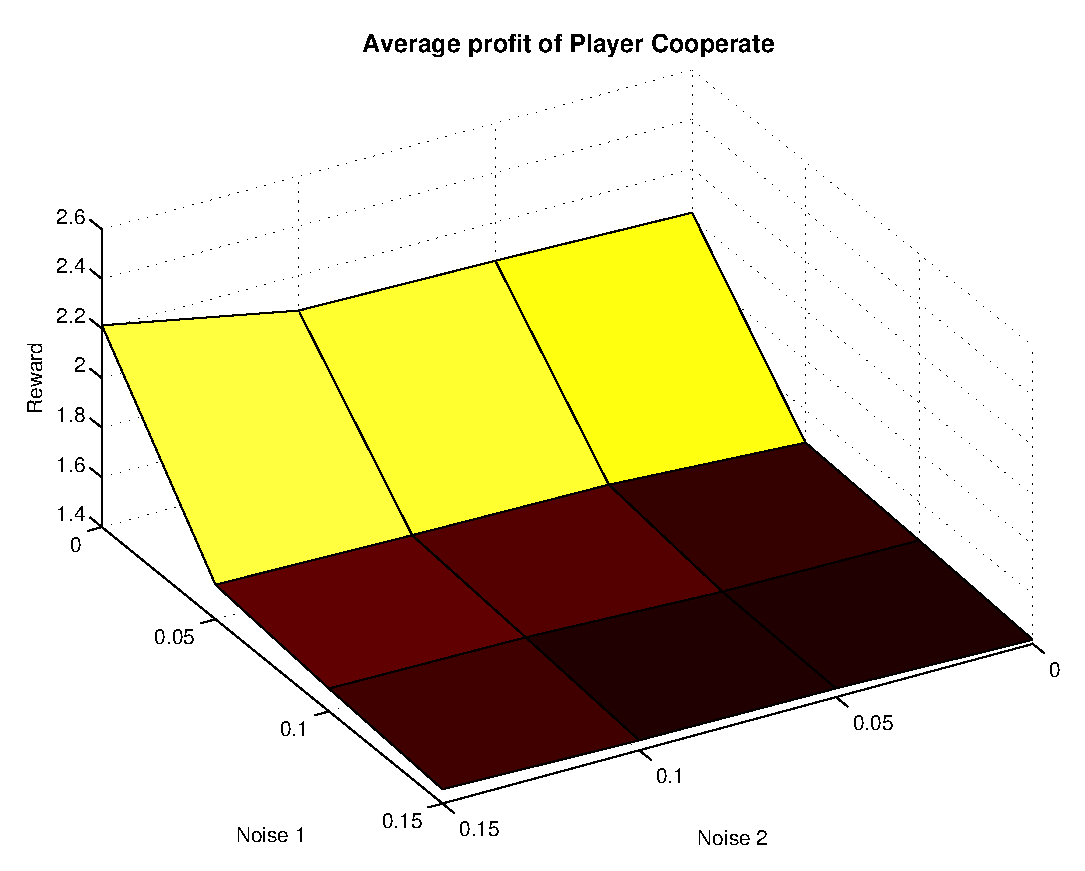
\includegraphics[width=\textwidth]{pics/simulation1/Reward_vs_Noise_of_Player_Cooperate}
\end{minipage}
\hfill
\begin{minipage}[hbt]{0.3\textwidth}
	\centering
	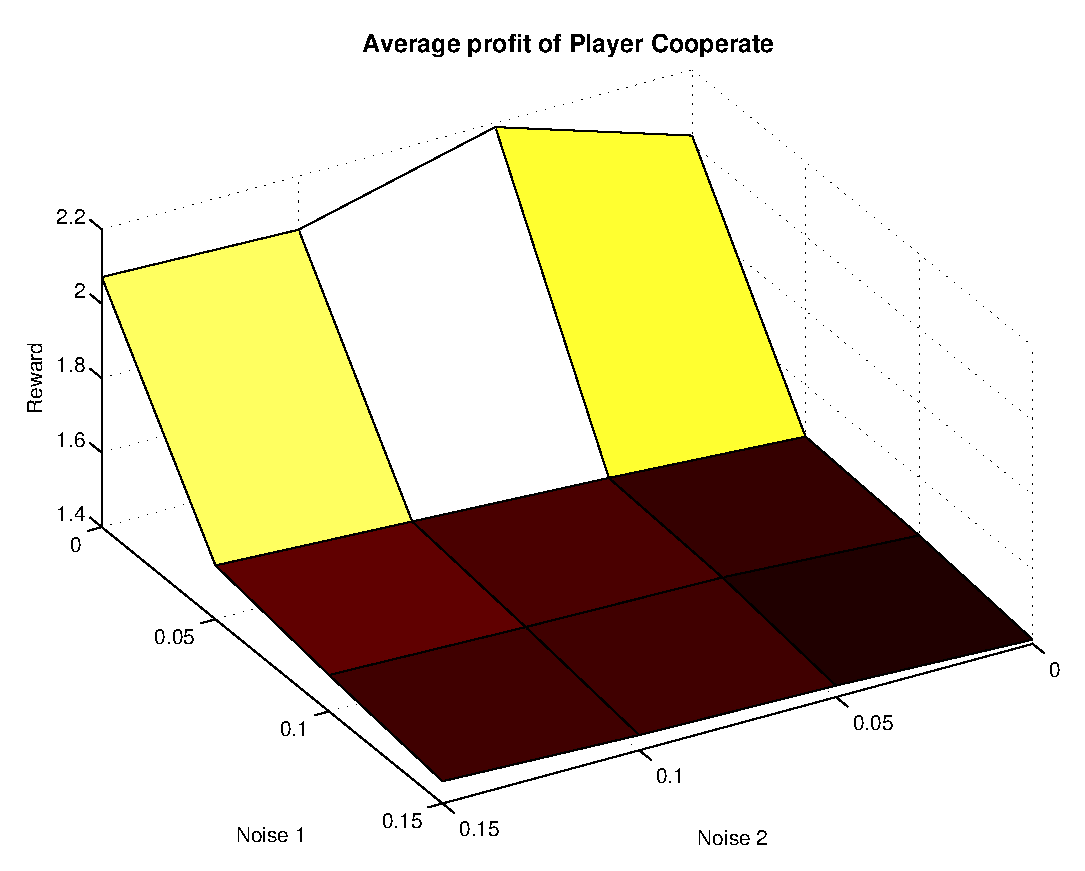
\includegraphics[width=\textwidth]{pics/simulation2/Reward_vs_Noise_of_Player_Cooperate}
\end{minipage}
	\caption{Reward plot of the Cooperative Player}
	\label{Pic Cooperative Player}
\end{figure}

In a situation of no noise, this player performs strong against mostly friendly players, but gets exploited by aggressive players. In this situation it performs better than always defect, but similar to random.\\

Because this player is cooperative and not reactive Noise2 doesn't matter. On the other hand performance drastically decreases with Noise1. The seemingly inserted rejections make other players explore defective moves. Because the defective moves are not retaliated the other players might then stick with these defective moves. Players that start exploiting this player are Friedmann, Pavlov, CDowning and LookBack CDowning.\\

In a situation with noise this strategy is still strong with TFT mutants, because a cooperative interaction gets restored in the fastest possible way.\\

Still with a drop of 0.7 to 0.8 in performance this player is one of the players that is the most susceptible to noise overall.\\

Traits of the player:

\renewcommand{\labelitemi}{}

\begin{itemize}
	\item + Can sustain cooperation with friendly players even in noise
	\item - Exploitable
	\item - Does not respond to the opponents move
\end{itemize}
\renewcommand{\labelitemi}{$\bullet$}

\subsubsection{Defective Player}

The player's performance in both simulations is shown in figure~\ref{pic player defect}.\\

\begin{figure}[h]

\begin{minipage}[hbt]{0.65\textwidth}
	\centering
	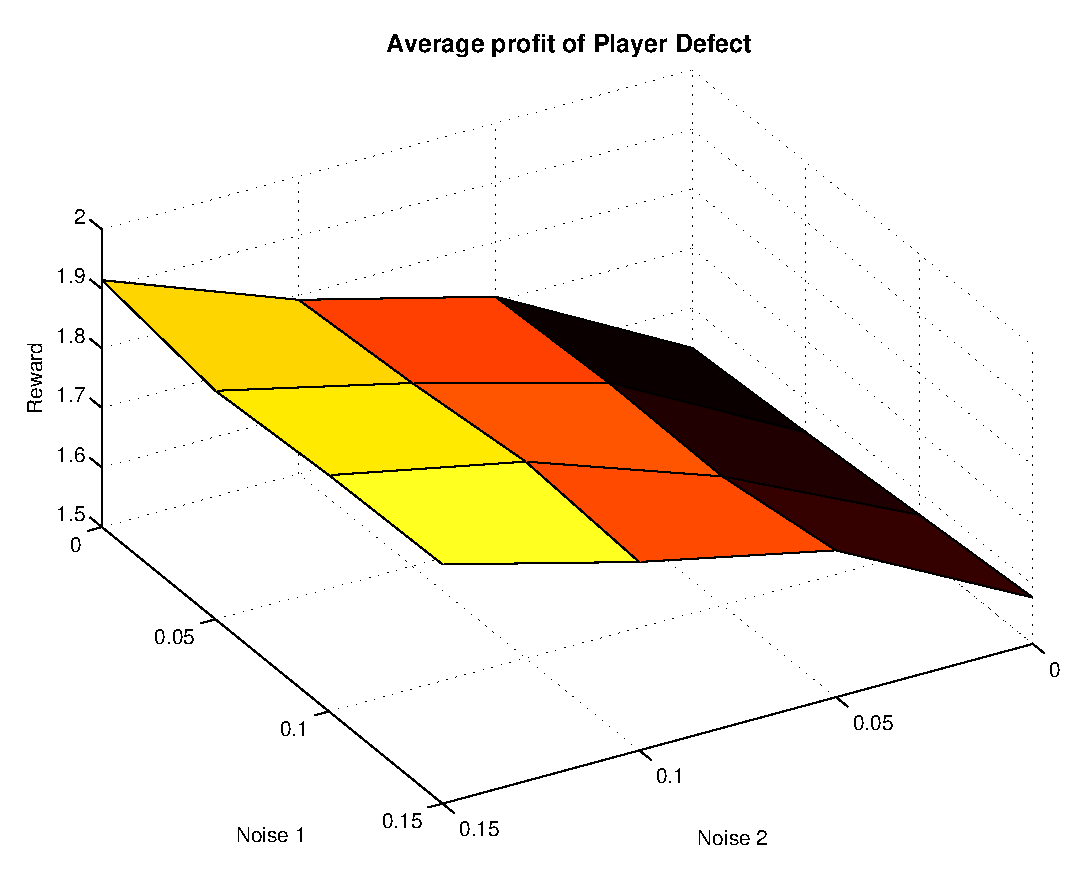
\includegraphics[width=\textwidth]{pics/simulation1/Reward_vs_Noise_of_Player_Defect}
\end{minipage}
\hfill
\begin{minipage}[hbt]{0.3\textwidth}
	\centering
	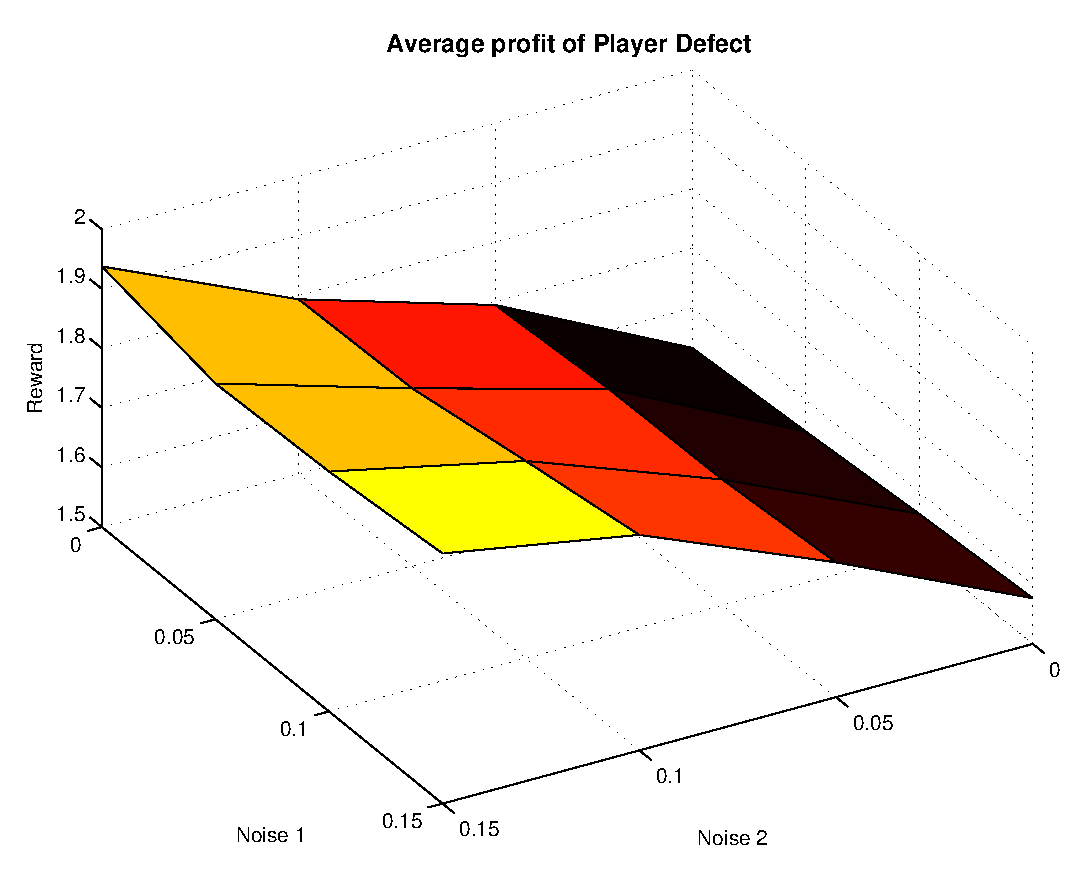
\includegraphics[width=\textwidth]{pics/simulation2/Reward_vs_Noise_of_Player_Defect}
\end{minipage}
	\caption{Reward plot of the Player Defect}
	\label{pic player defect}
\end{figure}

The player is so unfriendly, that Noise2 help him. A move where he can exploit the opponent gives him 5 times the reward of mutual defections, therefore even a small number of exploiting moves helps him a lot. If we would run the simulation with a Noise close to 50\% this player would become the most successful player. The performance increases in general against TFT mutants, but especially against players that try hard to avoid mutual defections, such as TF2T, reconciliation TFT, limited Reconciliation TFT. The strongest rise in performance comes against the player Evolutionary. \\

Traits of the player:

\renewcommand{\labelitemi}{}

\begin{itemize}
	\item + Can exploit players that do not respond
	\item + Performance increase with Noise
	\item - Ends up in mutual defections with most players

\end{itemize}
\renewcommand{\labelitemi}{$\bullet$}

\subsubsection{Random Player}
The player's performance in both simulations is shown in figure~\ref{pic player random}.\\
\begin{figure}[h]

\begin{minipage}[hbt]{0.65\textwidth}
	\centering
	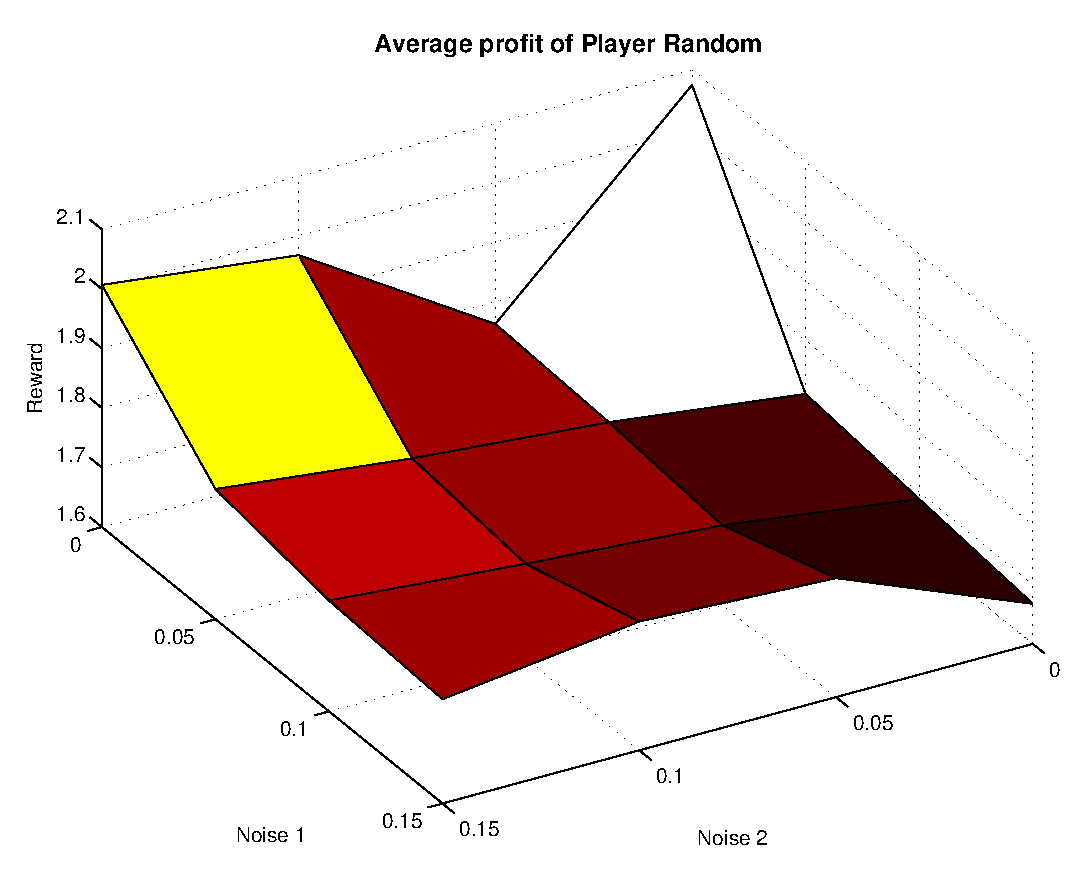
\includegraphics[width=\textwidth]{pics/simulation1/Reward_vs_Noise_of_Player_Random}
\end{minipage}
\hfill
\begin{minipage}[hbt]{0.3\textwidth}
	\centering
	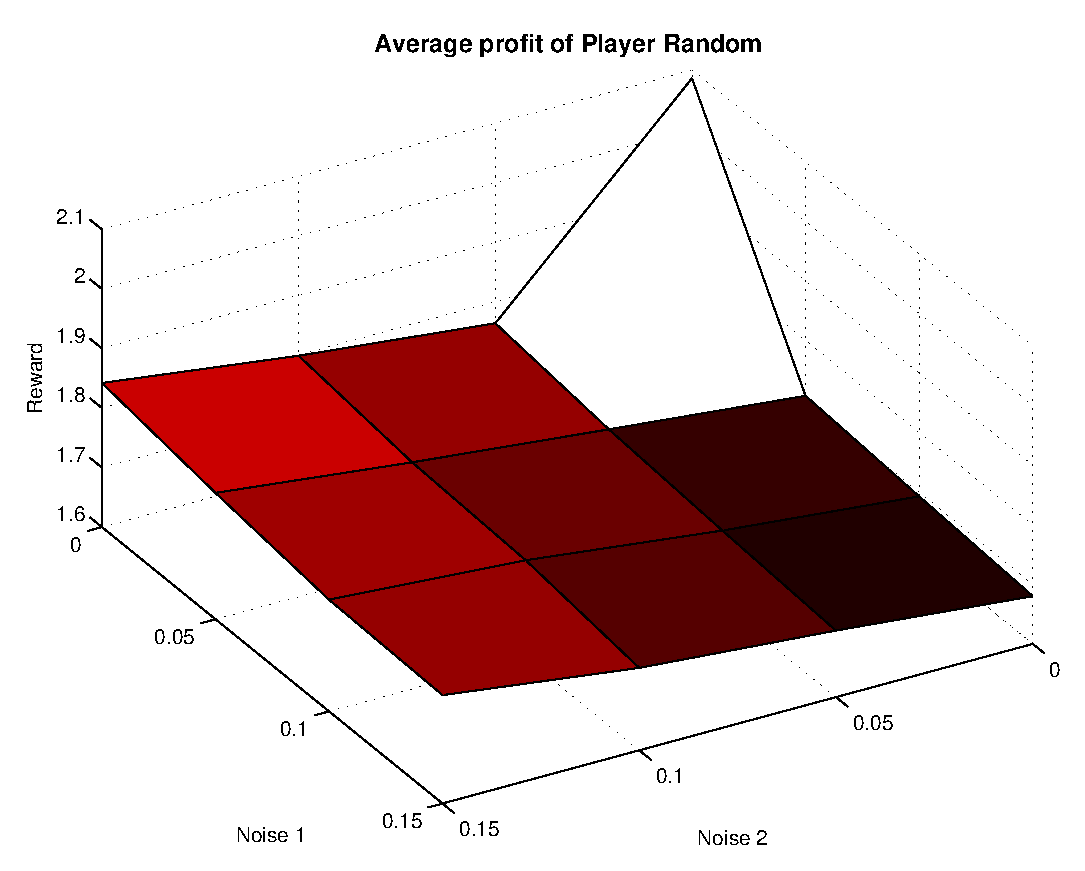
\includegraphics[width=\textwidth]{pics/simulation2/Reward_vs_Noise_of_Player_Random}
\end{minipage}
	\caption{Reward plot of the Random Player}
	\label{pic player random}
\end{figure}

The player does not get influenced that much by noise. There is a strange peak at zero noise, we were unable to find out why. If the noise makes his moves appear a little more cooperate there is a slight increase in performance, most likely due to more cooperative reactions from TFT mutants.

\subsubsection{Tit For Tat}
The player's performance in both simulations is shown in figure~\ref{pic player tit for tat}.\\
\begin{figure}[h]

\begin{minipage}[hbt]{0.65\textwidth}
	\centering
	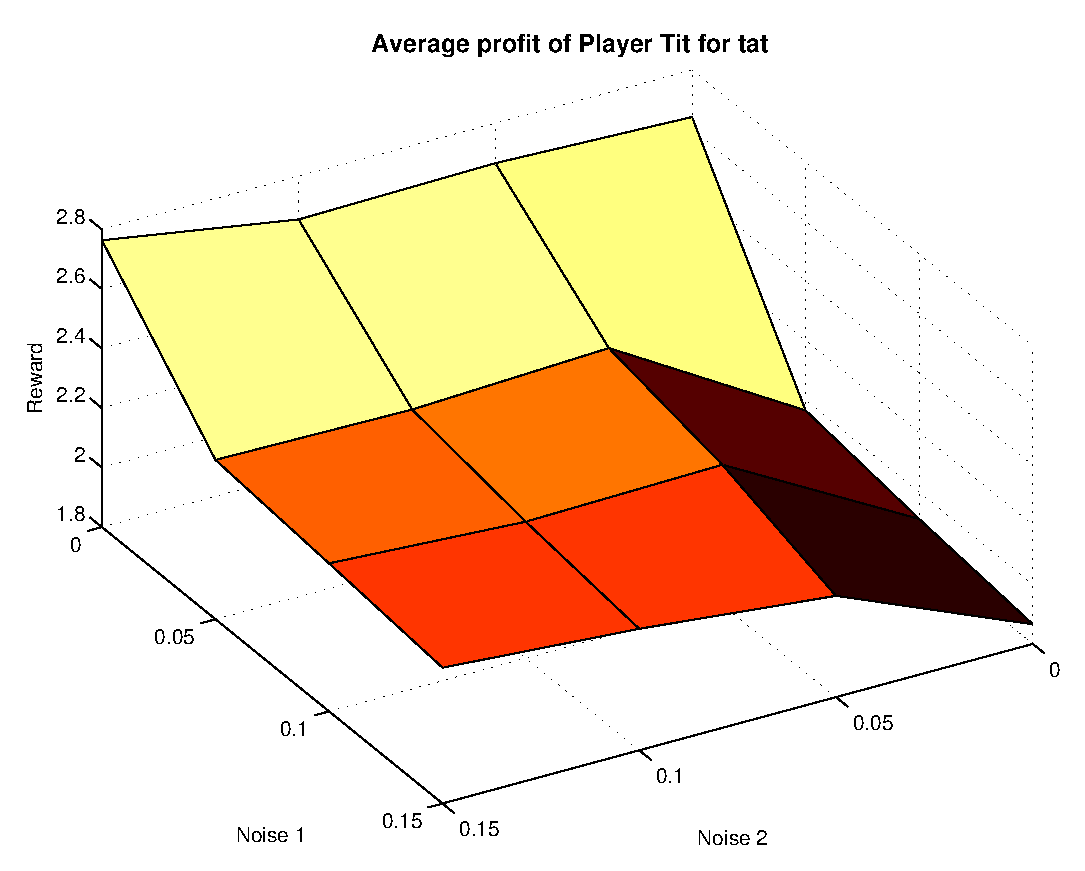
\includegraphics[width=\textwidth]{pics/simulation1/Reward_vs_Noise_of_Player_Tit_for_tat}
\end{minipage}
\hfill
\begin{minipage}[hbt]{0.3\textwidth}
	\centering
	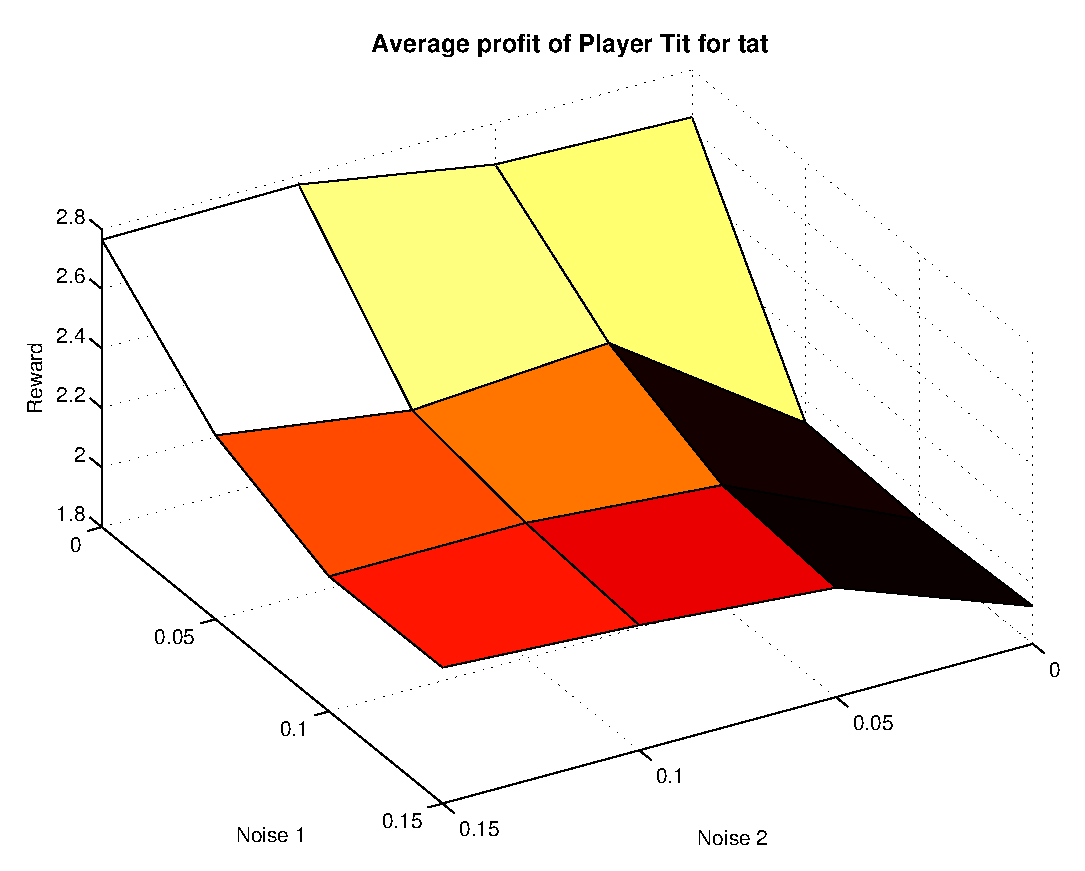
\includegraphics[width=\textwidth]{pics/simulation2/Reward_vs_Noise_of_Player_Tit_for_tat}
\end{minipage}
	\caption{Reward plot of the Player Tit For Tat}
	\label{pic player tit for tat}
\end{figure}

Tit for Tat (TFT) is a rather strong player. He won Axelrod's tournaments that were without noise. For Noise1=0 he is one of the strongest of all players. These graphs above show that this player is extremely susceptible to noise1. The reason is that with no noise 1 he will always cooperate with other TFT mutants because the first move was cooperative. With noise the first move maters less. There are basically three states he can enter with himself.\\

\renewcommand{\labelitemi}{}

\begin{itemize}
	\item State 1: Mutual cooperation. Performance 3
	\item State 2: Alternating defection and cooperation. Performance 2.5
	\item State 3: Mutual defection. Performance 1
\end{itemize}

 A Noise1 signal changes the state from state 1 to state 2 or state 2 to state 3. Noise2 works in the other direction. The two noises are basically transition probabilities. For Noise1 greater than zero and Noise2 equal to zero the TFT ends up stuck in state three with itself. For equal noises in both directions TFT should be 50\% of the time in state 2 and 25\% in the states 1 and 3. This would imply the performance: 
$0.25*3+0.5*2.5+0.25*1=2.25$\\
Table~\ref{tab:tfttable} shows the performance of TFT against itself. Because the players in our simulation could only perform mirrored decisions state 2 was impossible and the actual performance was somewhat lower.

\begin{table}[h]
 \begin{center}
\caption{Performance of TFT playing against TFT}\label{tab:tfttable} \vspace{3mm}
\begin{tabular}{|l|c|c|c|c|c|}
\hline
   	& Noise 2 = 0 & Noise 2 = 0.05& Noise 2 = 0.1& Noise 2 = 0.15 \\
  \hline
  Noise 1 = 0 	& 3.0000	 &3.0000 	&3.0000	&3.0000 \\
 \hline
  Noise 1 = 0.05	 & 1.0016	 &2.0127 	&2.3438	&2..4745 \\
 \hline
  Noise 1 = 0.10 	& 1.0018	 &1.6184 	&1.9847	&2.1967 \\
 \hline
  Noise 1 = 0.15 	& 1.0011	 &1.5170 	&1.7666	&2.0086 \\
 \hline
\end{tabular}
 \end{center}


\end{table}

\begin{table}[h]
 \begin{center}
\caption{Cooperation of TFT depending on the Noise} \vspace{3mm}
\begin{tabular}{|l|c|c|c|c|c|}
\hline
   	& Noise 2 = 0 & Noise 2 = 0.05& Noise 2 = 0.1& Noise 2 = 0.15 \\
  \hline
  Noise 1 = 0 	& 0.8075	 &0.8247 	&0.8351	&0.8917 \\
 \hline
  Noise 1 = 0.05	 & 0.3958	&    0.5967&    0.6192 &   0.6516 \\
 \hline
  Noise 1 = 0.10 	& 0.3418 &   0.5127 &   0.5428&   0.5866 \\
 \hline
  Noise 1 = 0.15 	& 0.2886  &  0.4240 &   0.4836  &  0.5297 \\
 \hline
\end{tabular}
 \end{center}
\end{table}

Already at Noise1=0.05 the number of cooperative moves TFT performs drops from 40 to 80 percent. At higher Noise2 with no Noise1 the number of defections performed by TFT halves.\\

Traits of the player:

\renewcommand{\labelitemi}{}

\begin{itemize}
	\item + Responds fast
	\item + Not exploitable
	\item + Forgiving
	\item - Only accepts an apology, but does not initiate it himself, so he can stuck in mutual defections!
\end{itemize}
\renewcommand{\labelitemi}{$\bullet$}

\subsubsection{Friedmann}
The player's performance in both simulations is shown in figure~\ref{pic player friedmann}.\\
\begin{figure}[h]

\begin{minipage}[hbt]{0.65\textwidth}
	\centering
	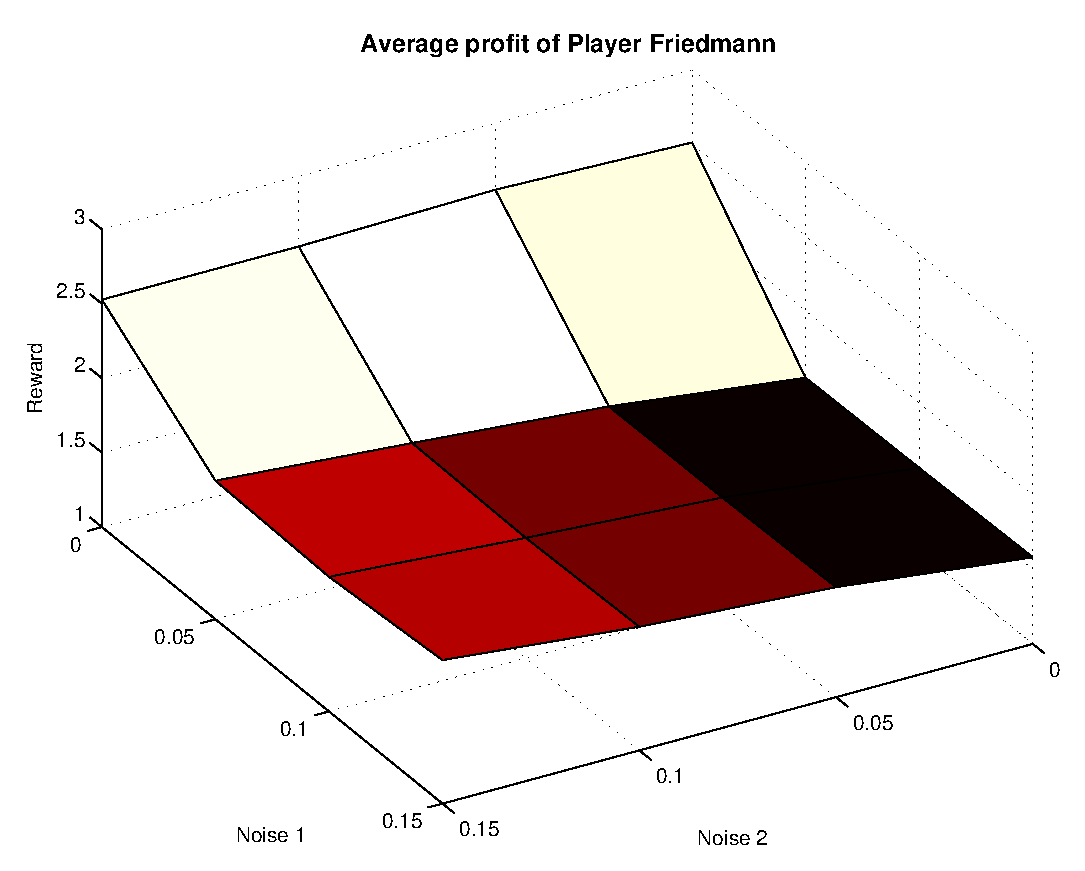
\includegraphics[width=\textwidth]{pics/simulation1/Reward_vs_Noise_of_Player_Friedmann}
\end{minipage}
\hfill
\begin{minipage}[hbt]{0.3\textwidth}
	\centering
	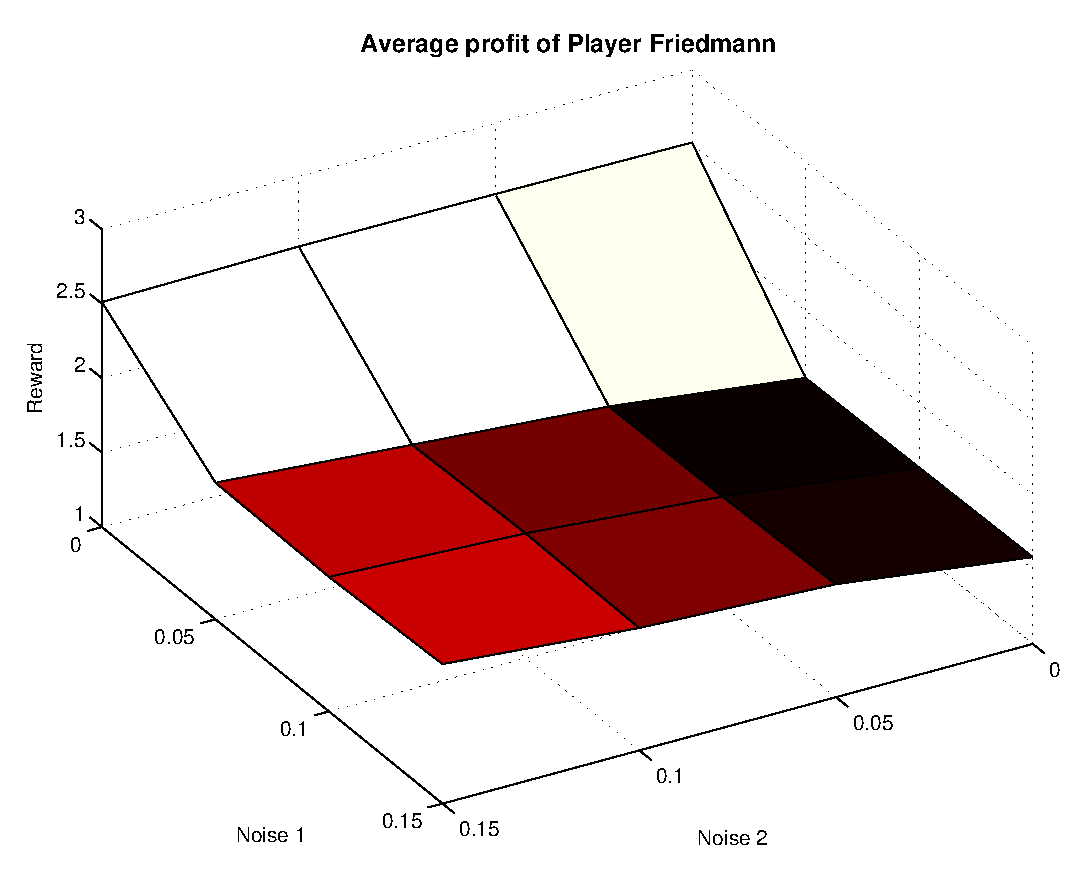
\includegraphics[width=\textwidth]{pics/simulation2/Reward_vs_Noise_of_Player_Friedmann}
\end{minipage}
	\caption{Reward plot of the Player Friedmann}
	\label{pic player friedmann}
\end{figure}

In the case of perfect information this player can profit from mutual cooperation with many players. In this case he performs well. However for any Noise1 greater than zero the player will receive a rejection at some point and therefore act like the player "Defect" most of the time. Friedmann generally tries to retaliate so hard on a rejection that the other player will not even attempt one rejection. However Friedmann cannot capitalise on this deterrent effect, because the moment the opponent realises it is already too late and he cannot know it in advance.\\

\begin{table}[h]
 \begin{center}
\caption{Cooperation of Friedmann dependant on the Noise} \vspace{3mm}
\begin{tabular}{|l|c|c|c|c|c|}
\hline
   	& Noise 2 = 0 & Noise 2 = 0.05& Noise 2 = 0.1& Noise 2 = 0.15 \\
  \hline
  Noise 1 = 0 	& 0.6002&    0.6000&    0.6000 &   0.6000 \\
 \hline
  Noise 1 = 0.05	 & 0.0004&    0.0001 &   0.0001  &  0.0001 \\
 \hline
  Noise 1 = 0.10 	& 0.0001  &  0.0001&    0.0001 &   0.00016 \\
 \hline
  Noise 1 = 0.15 	& 0.0001  &  0.0001  &  0.0001  &  0.0001 \\
 \hline
\end{tabular}
 \end{center}
\end{table}

As soon as Noise1 is greater than 0 the number of cooperative moves goes to zero. But already at zero noise Friedmann only has 60\% cooperative moves, while TFT has 80\%.\\


Traits of the player:

\renewcommand{\labelitemi}{}

\begin{itemize}
	\item + Stays in mutual cooperation with friendly players when Noise1 is zero
	\item - Completely breaks down with Noise1 greater than zero
\end{itemize}
\renewcommand{\labelitemi}{$\bullet$}

\subsubsection{Pavlov}
The player's performance in both simulations is shown in figure~\ref{pic player pavlov}.\\
\begin{figure}[h]

\begin{minipage}[hbt]{0.65\textwidth}
	\centering
	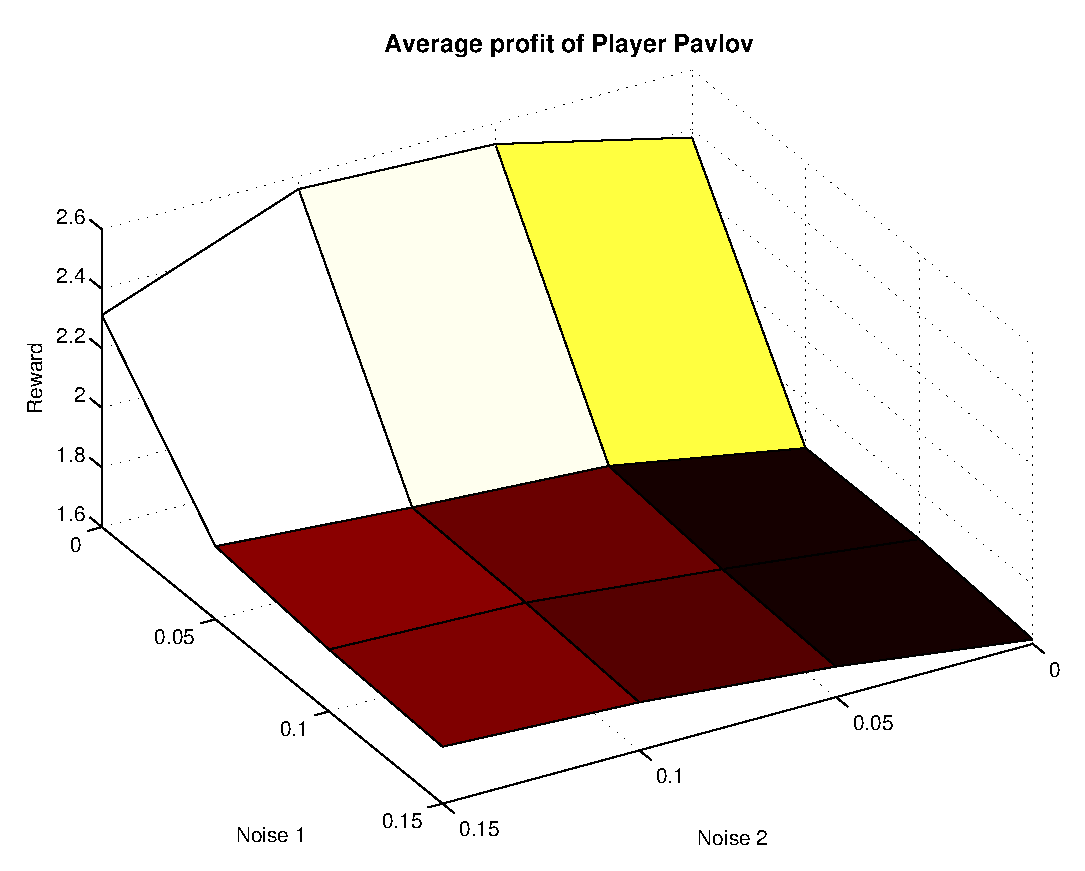
\includegraphics[width=\textwidth]{pics/simulation1/Reward_vs_Noise_of_Player_Pavlov}
\end{minipage}
\hfill
\begin{minipage}[hbt]{0.3\textwidth}
	\centering
	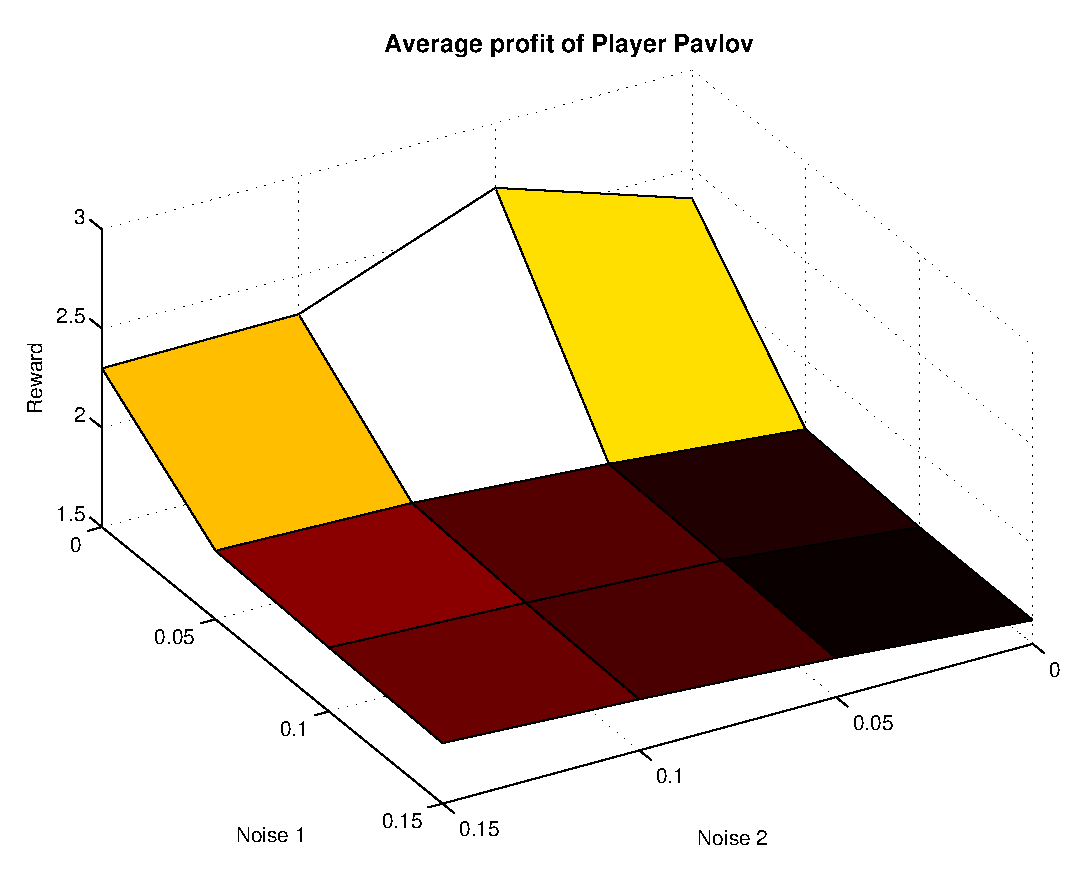
\includegraphics[width=\textwidth]{pics/simulation2/Reward_vs_Noise_of_Player_Pavlov}
\end{minipage}
	\caption{Reward plot of the Player pavlov}
	\label{pic player pavlov}
\end{figure}

Pavlov performs rather well without Noise1. If Noise1 is greater then zero, some players realise that defections against Pavlov work as well as cooperations. Pure defect against Pavlov results in the rewards 5 1 5 1 5 1 for the opponent, while pure cooperation results in 3 3 3 3, given Pavlov is cooperative when the opponent started playing random. With zero noise the opponent gets an average reward of 3 for cooperation and defection but with noise the performance of cooperation decreases (because Pavlov retaliates). Players that largely start to defect against Pavlov are:  Friedmann, Tit for average Tat, CDowning, LookBack CDowning and the Strategy switcher.

\begin{table}[h]
 \begin{center}
\caption{Cooperation of Pavlov depending on the Noise} \vspace{3mm}
\begin{tabular}{|l|c|c|c|c|c|}
\hline
   	& Noise 2 = 0 & Noise 2 = 0.05& Noise 2 = 0.1& Noise 2 = 0.15 \\
  \hline
  Noise 1 = 0 	&     0.8239 &   0.8488&    0.8541&    0.8037 \\
 \hline
  Noise 1 = 0.05	 &   0.4885  &  0.5433 &   0.5697  &  0.5860 \\
 \hline
  Noise 1 = 0.10 	& 0.4939  &  0.5211 &   0.5338 &   0.5455 \\
 \hline
  Noise 1 = 0.15 	& 0.5063    &0.5187  &  0.5251 &   0.5319 \\
 \hline
\end{tabular}
 \end{center}
\end{table}

Without Noise 1 the number of Cooperative moves is around 80\% while it is around 50\% with Noise 1. It is interessting that with Noise2 but no Noise1 Pavlov is less cooperative than TFT.\\


Traits of the player:

\renewcommand{\labelitemi}{}
\begin{itemize}
	\item + Forgives fast
	\item + Initializes cooperation out of mutual defection
	\item + Not exploitable without noise
	\item - Too many cooperative moves against defecting players
	\item - Not retaliating (pure defect and pure cooperation perform equally well)
\end{itemize}
\renewcommand{\labelitemi}{$\bullet$}

\subsubsection{Tit For 2 Tat}
The player's performance in both simulations is shown in the two figures below:
\begin{figure}[h]

\begin{minipage}[hbt]{0.65\textwidth}
	\centering
	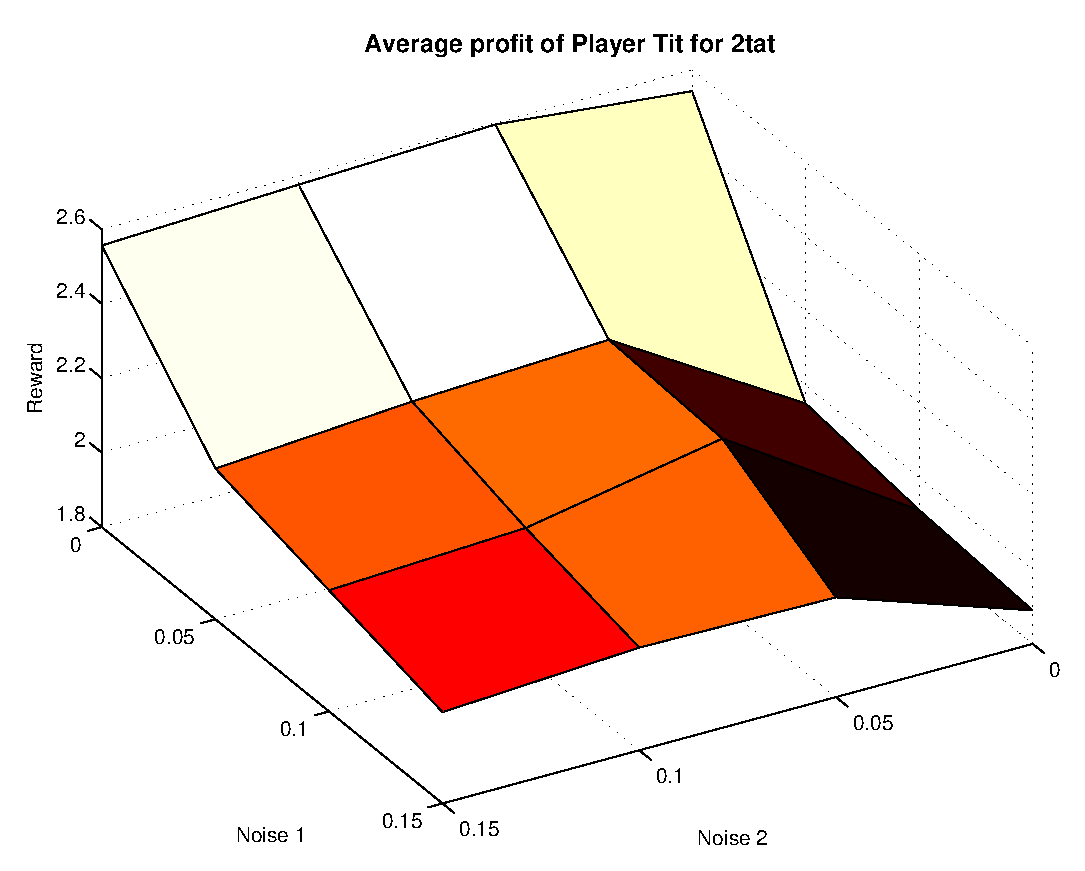
\includegraphics[width=\textwidth]{pics/simulation1/Reward_vs_Noise_of_Player_Tit_for_2tat}
\end{minipage}
\hfill
\begin{minipage}[hbt]{0.3\textwidth}
	\centering
	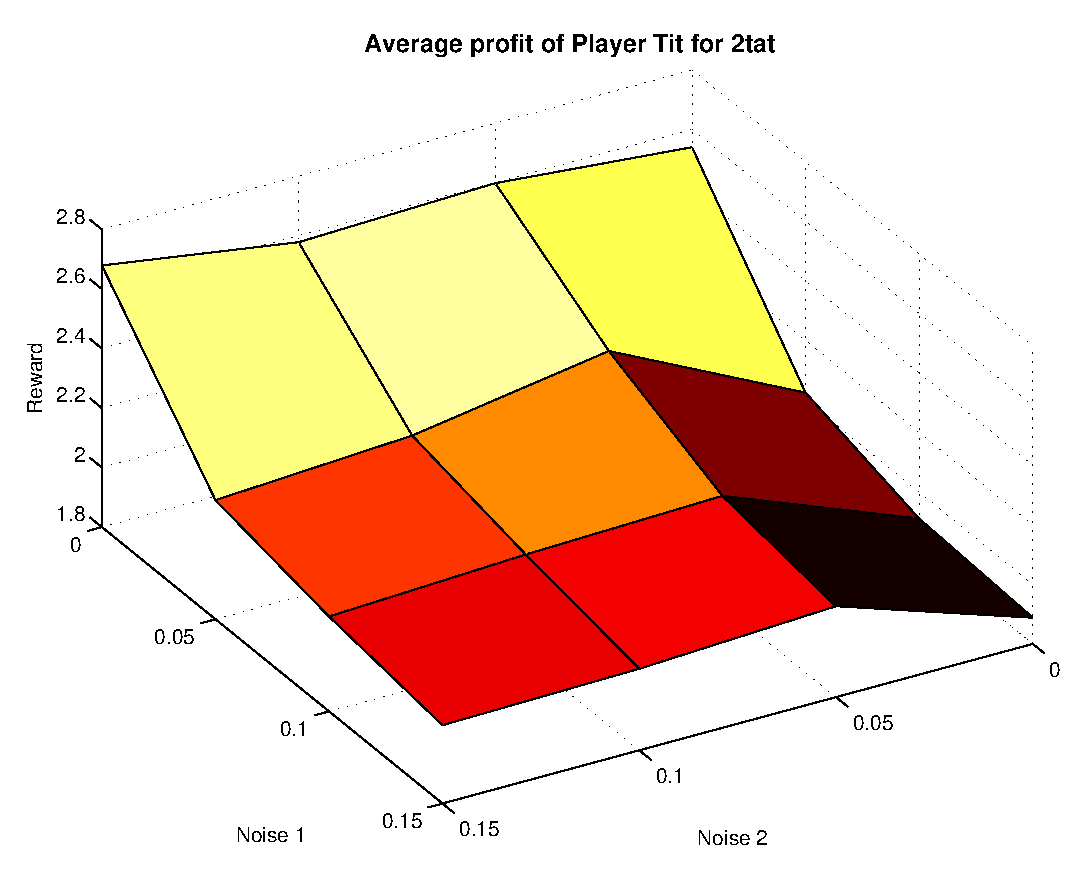
\includegraphics[width=\textwidth]{pics/simulation2/Reward_vs_Noise_of_Player_Tit_for_2tat}
\end{minipage}
	\caption{Reward plot of the Player Tit For 2 Tat}
	\label{pic player tf2t}
\end{figure}

As a TFT mutant it has a similar performance. The difference is that this player is more forgiving. The bad thing is that this makes him exploitable. The better thing is that it is more robust to Noise1 as it does not react to single defections. The player still ends up in mutual defections with itself if Noise2 is zero and Noise1 greater than zero, but for both Noises greater than zero the player plays much stronger against itself. At zero noise the performance of TF2T is worse than the one of TFT, but with Noise1 their performances are similar. The effect that players like "Evolutionary" will exploit TF2T seems to balance out with the better resistance to noise.

\begin{table}[h]
 \begin{center}
\caption{Cooperation of TF2T depending on the Noise} \vspace{3mm}
\begin{tabular}{|l|c|c|c|c|c|}
\hline
   	& Noise 2 = 0 & Noise 2 = 0.05& Noise 2 = 0.1& Noise 2 = 0.15 \\
  \hline
  Noise 1 = 0 	&        0.8271&    0.8796 &   0.8880  & 0.8947 \\
 \hline
  Noise 1 = 0.05	 &       0.5366  &  0.7450  &  0.7712 &   0.7926 \\
 \hline
  Noise 1 = 0.10 	&    0.5132 &   0.7349  &  0.7375&   0.7622 \\
 \hline
  Noise 1 = 0.15 	&     0.4864 &   0.6503 &   0.6977   & 0.72749 \\
 \hline
\end{tabular}
 \end{center}
\end{table}

The cooperation stays much higher than for TFT especially if Noise2 also is not zero.

Traits different to TFT:

\renewcommand{\labelitemi}{}
\begin{itemize}
	\item + More Forgiving
	\item - More Exploitable
\end{itemize}
\renewcommand{\labelitemi}{$\bullet$}
 
\subsubsection{Joss}
The player's performance in both simulations is shown in the two figures below:
\begin{figure}[h]

\begin{minipage}[hbt]{0.65\textwidth}
	\centering
	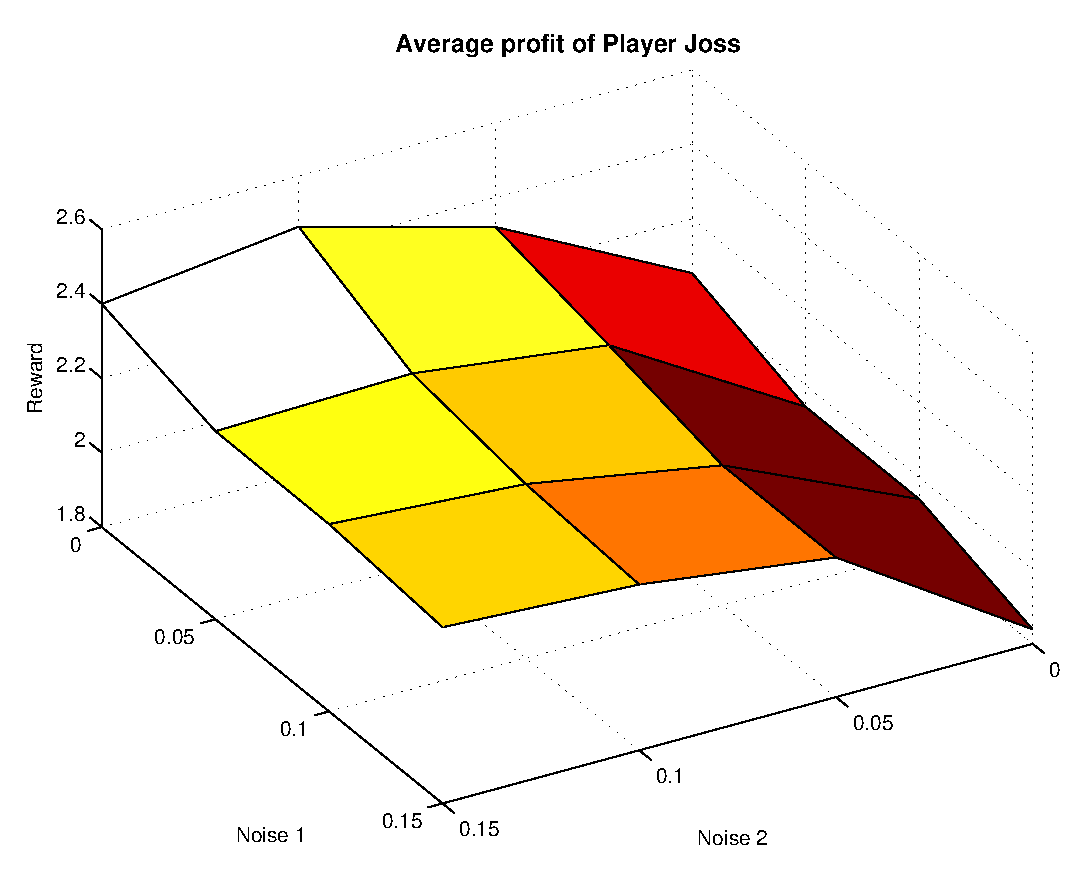
\includegraphics[width=\textwidth]{pics/simulation1/Reward_vs_Noise_of_Player_Joss}
\end{minipage}
\hfill
\begin{minipage}[hbt]{0.3\textwidth}
	\centering
	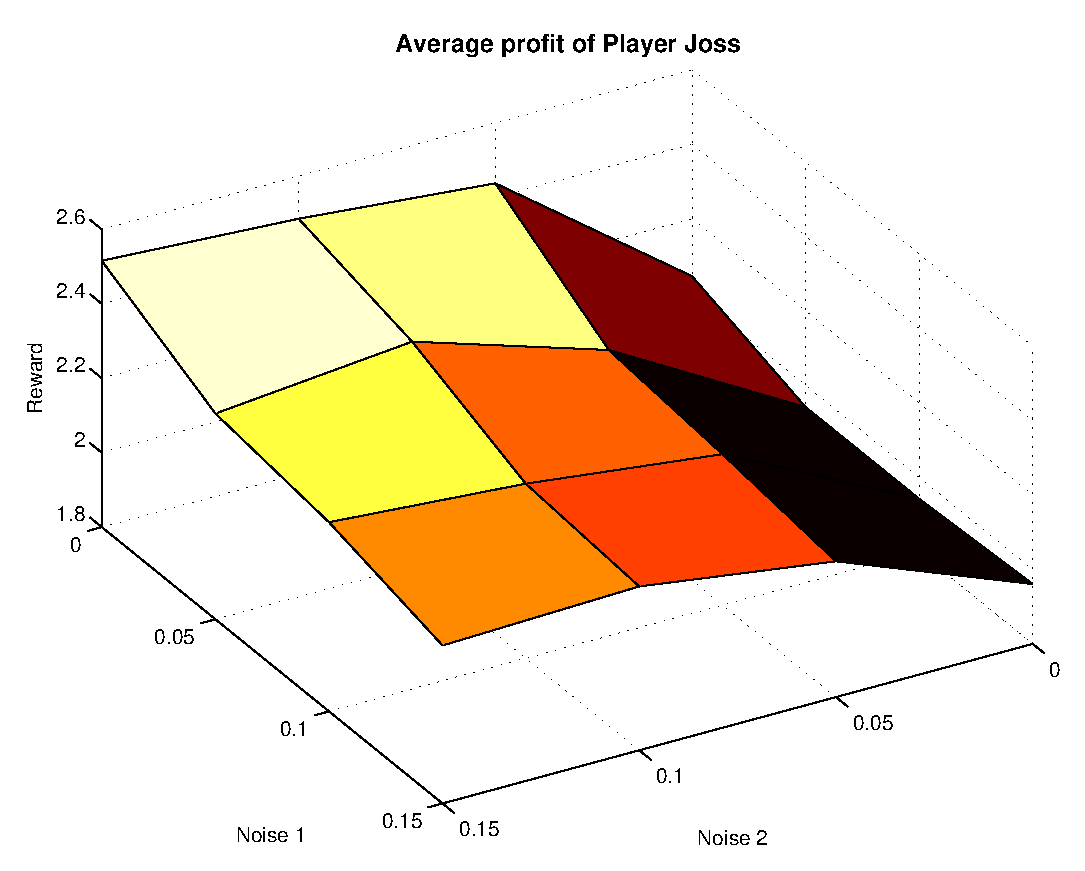
\includegraphics[width=\textwidth]{pics/simulation2/Reward_vs_Noise_of_Player_Joss}
\end{minipage}
	\caption{Reward plot of the Player Joss}
	\label{pic player joss}
\end{figure}

While this is a TFT mutant, its performance dependence on noise looks totally different. The player generally performs poorly. At some noises this player is able to exploit TF2T (Noise2 greater than 0 and Noise1 0) however most of the time the retaliation of the defections outweighs their gain. TFT is very susceptible to Noise1 and Joss makes himself look like under Noise1 to his opponent. It is interesting that the performance of this player looks like the performance of "Defect" just shifted about 0.5 upwards.

\begin{table}[h]
 \begin{center}
\caption{Cooperation of Joss depending on the Noise} \vspace{3mm}
\begin{tabular}{|l|c|c|c|c|c|}
\hline
   	& Noise 2 = 0 & Noise 2 = 0.05& Noise 2 = 0.1& Noise 2 = 0.15 \\
  \hline
  Noise 1 = 0 	&            0.3983  &  0.5300  &  0.6102  &  0.6172 \\
 \hline
  Noise 1 = 0.05	 &          0.3983 &   0.5300  &  0.6102 &  0.6172 \\
 \hline
  Noise 1 = 0.10 	&        0.2968  &  0.4026  &  0.4625    &0.5006 \\
 \hline
  Noise 1 = 0.15 	&     0.2404    &0.3720 &   0.4225  &  0.4591 \\
 \hline
\end{tabular}
 \end{center}
\end{table}

With higher Noise2 some cooperation can be achieved, but generally the player is mostly defecting.

Traits different to TFT:

\renewcommand{\labelitemi}{}
\begin{itemize}
	\item - initates defections
\end{itemize}
\renewcommand{\labelitemi}{$\bullet$}
%%%%%


%%%%%
\newpage
\subsubsection{Diekmann}
The player's performance in both simulations is shown in the two figures below:
\begin{figure}[h]

\begin{minipage}[hbt]{0.65\textwidth}
	\centering
	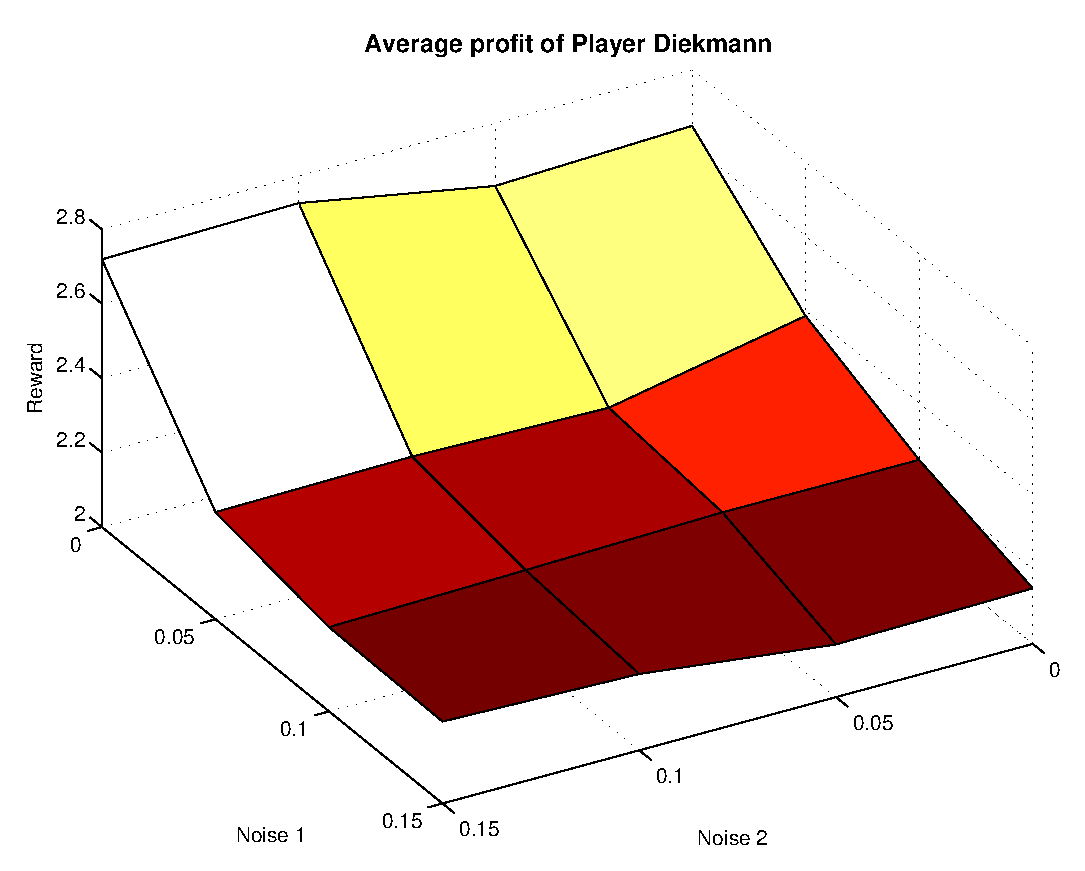
\includegraphics[width=\textwidth]{pics/simulation1/Reward_vs_Noise_of_Player_Diekmann}
\end{minipage}
\hfill
\begin{minipage}[hbt]{0.3\textwidth}
	\centering
	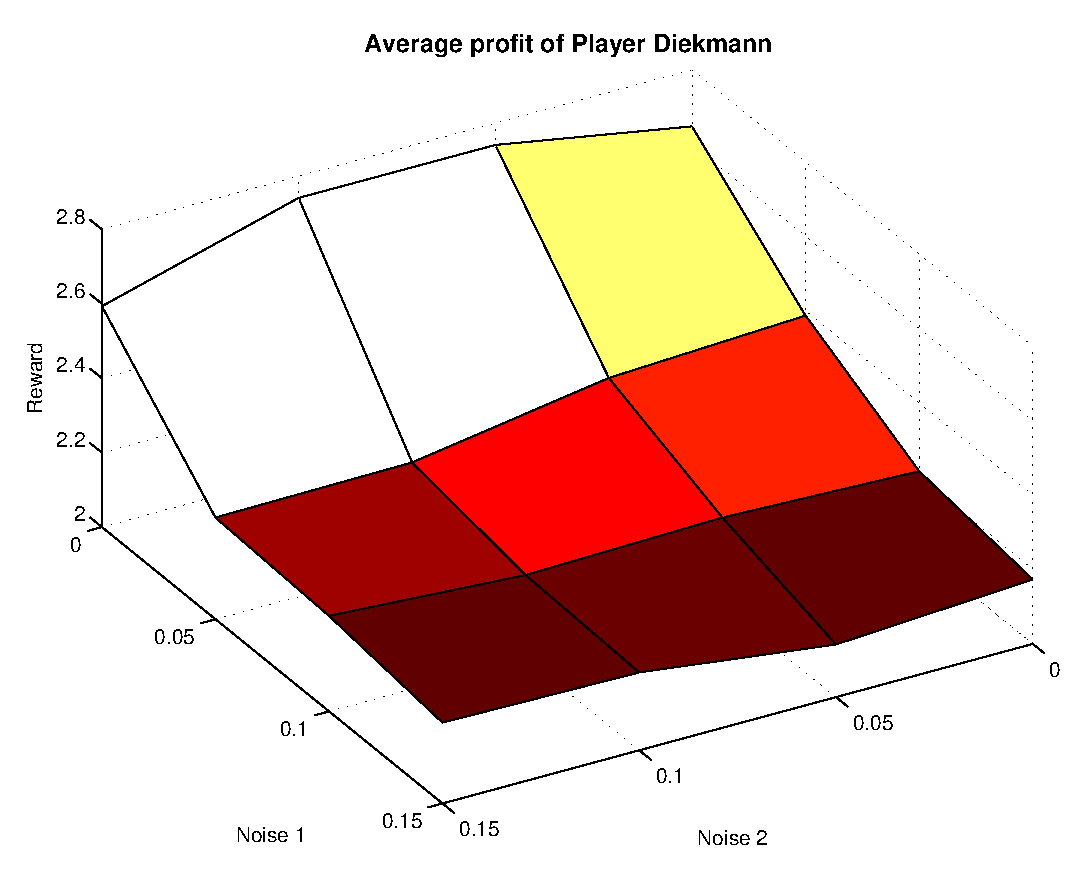
\includegraphics[width=\textwidth]{pics/simulation2/Reward_vs_Noise_of_Player_Diekmann}
\end{minipage}
	\caption{Reward plot of the Player Diekmann}
	\label{pic player diekmann}
\end{figure}

This is a TFT mutant, that performs on the same level as TFT at no noise, and is therefore one of the strongest players if there is no noise. While his performance also drops with Noise1 the effect is much less severe. For Noise1=0.05 and Noise2=0, TFT drops about 0.9, while Diekmann only drops 0.5. This player actually initiates cooperation and gets not stuck in mutual defection with TFT mutants. The weakness of this player is that he is exploitable by defective moves every 10 moves. However on our simulation we haven't seen a player exploiting this weakness. Evolutionary could exploit it if the period in which the algorithm updates would be a multiple of the period in which Diekmann inserts cooperative moves.

\begin{table}[h]
 \begin{center}
\caption{Cooperation of Diekmann depending on the noise} \vspace{3mm}
\begin{tabular}{|l|c|c|c|c|c|}
\hline
   	& Noise 2 = 0 & Noise 2 = 0.05& Noise 2 = 0.1& Noise 2 = 0.15 \\
  \hline
  Noise 1 = 0 	&               0.8635 &   0.9034   & 0.9113 &  0.8741 \\
 \hline
  Noise 1 = 0.05	 &            0.7157 &   0.7263  &  0.7200  &  0.7359 \\
 \hline
  Noise 1 = 0.10 	&           0.6230  &  0.6500  &  0.6655 &   0.6946 \\
 \hline
  Noise 1 = 0.15 	&   0.5760 &   0.5895  &  0.6283 &   0.6496 \\
 \hline
\end{tabular}
 \end{center}
\end{table}

The cooperation drops not nearly as much with the Noise as this is the case for TFT, he even is much more cooperative at no noise. At low noise2 values he is more cooperative than TF2T, but when both noises get high TF2T is more cooperative.

Traits different to TFT:

\renewcommand{\labelitemi}{}
\begin{itemize}
	\item + initates cooperation
	\item - More Exploitable
\end{itemize}
\renewcommand{\labelitemi}{$\bullet$}
 
\subsubsection{Tit For Average Tat}
The player's performance in both simulations is shown in the two figures below:
\begin{figure}[h]

\begin{minipage}[hbt]{0.65\textwidth}
	\centering
	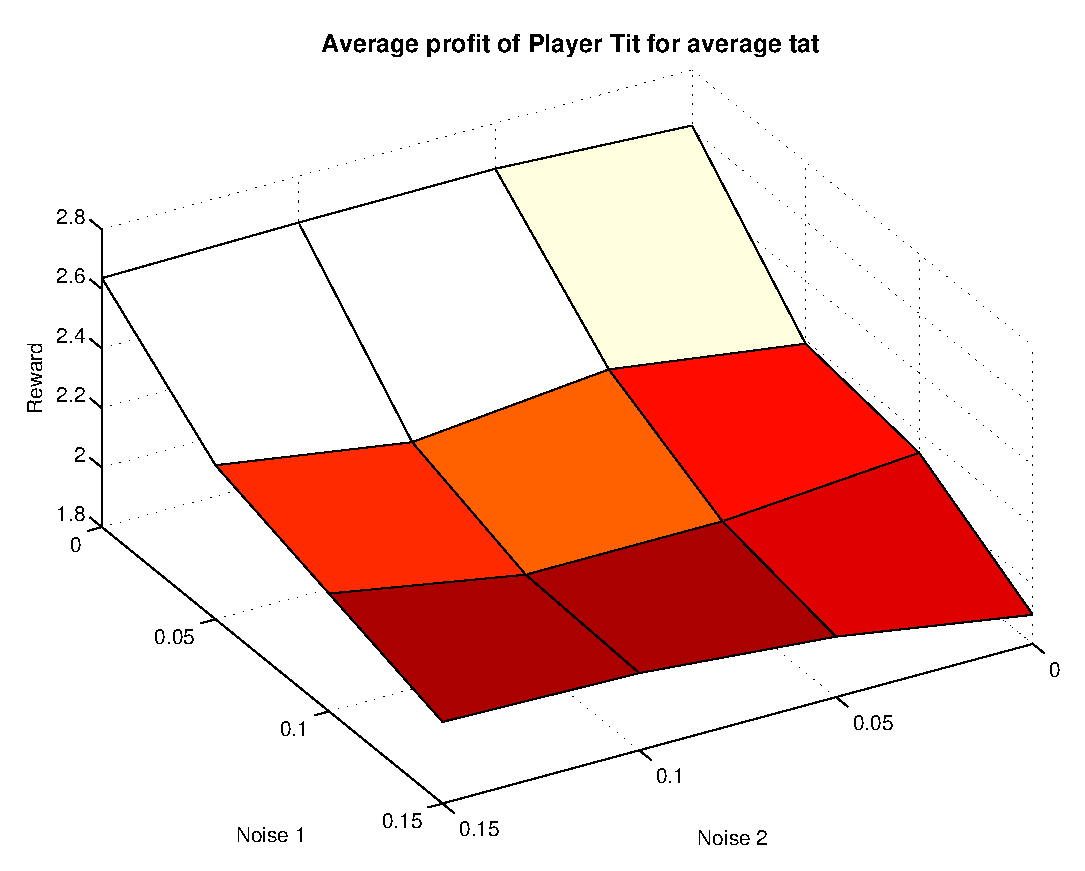
\includegraphics[width=\textwidth]{pics/simulation1/Reward_vs_Noise_of_Player_Tit_for_average_tat}
\end{minipage}
\hfill
\begin{minipage}[hbt]{0.3\textwidth}
	\centering
	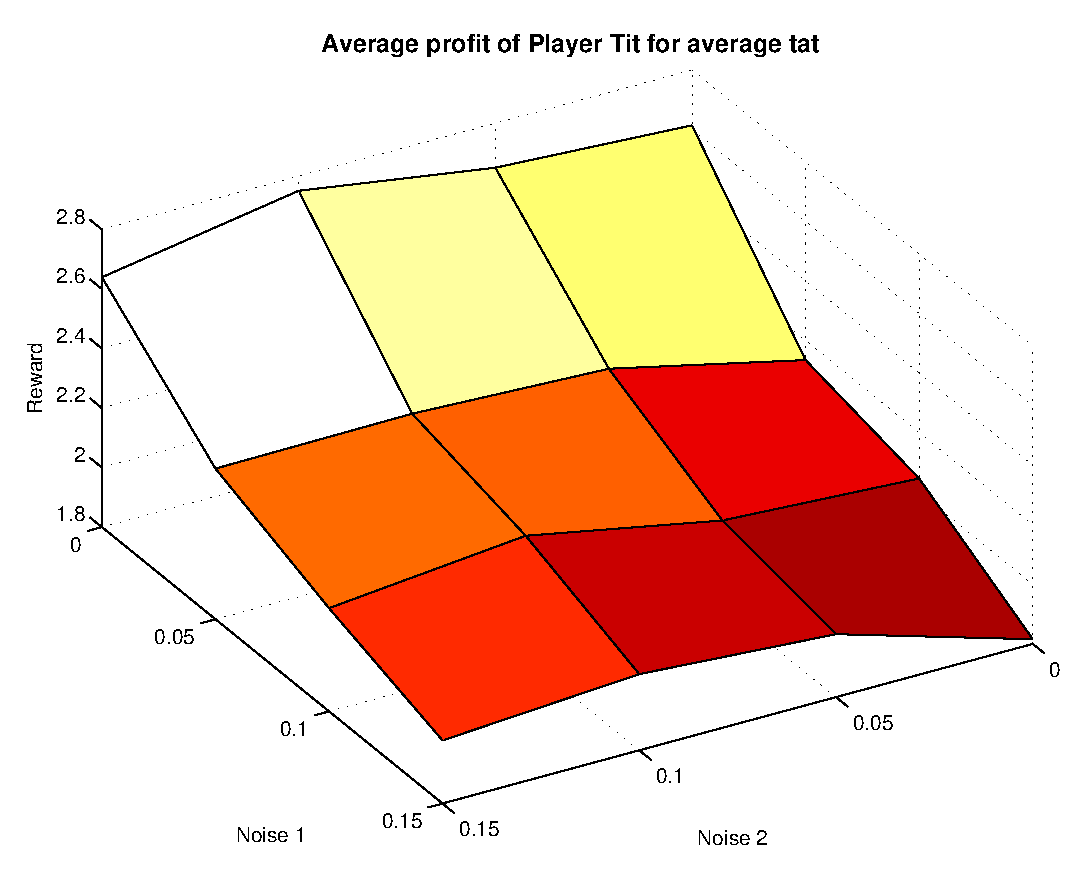
\includegraphics[width=\textwidth]{pics/simulation2/Reward_vs_Noise_of_Player_Tit_for_average_tat}
\end{minipage}
	\caption{Reward plot of the Player Tit For Average Tat}
	\label{pic player tfat}
\end{figure}

This TFT mutant looks very similar to Diekmann and other friendlier TFT mutants. The fact that it reacts to the players average move during the last turns allows him to ignore some of the noise. The problem is that if mutual defection appears it is just as hard to get out of it as it was to get into it. Maybe this players performance would have decreased if the simulation was run even longer. In general this player performs about as well as Reconciliation TFT and a little bit worse than Diekmann. Theoretically this player is exploitable. 

\begin{table}[h]
 \begin{center}
\caption{Cooperation of Tit For Average Tat depending on the noise} \vspace{3mm}
\begin{tabular}{|l|c|c|c|c|c|}
\hline
   	& Noise 2 = 0 & Noise 2 = 0.05& Noise 2 = 0.1& Noise 2 = 0.15 \\
  \hline
  Noise 1 = 0 	&    0.8056  &  0.8404  &  0.8456  &  0.8547 \\
 \hline
  Noise 1 = 0.05	 &     0.5316  &  0.6170 &   0.6140   & 0.6863 \\
 \hline
  Noise 1 = 0.10 	&    0.4712  &  0.4860  &  0.5100  &  0.5985 \\
 \hline
  Noise 1 = 0.15 	&       0.3419  &  0.4134 &   0.4660 &   0.5098 \\
 \hline
\end{tabular}
 \end{center}
\end{table}

The cooperation drops surprisingly fast with Noise1, but still not as fast as for TFT. The number of cooperative moves is still more similar to TFT than Diekmann. This is surprising, that the performances look so close, while the underlying moves are so different. Diekmanns very nice approach seems to be just as efficient as TFAT's more retaliating method. 

Traits of the player:

\renewcommand{\labelitemi}{}
\begin{itemize}
	\item + ignores single moves
	\item - Exploitable
\end{itemize}
\renewcommand{\labelitemi}{$\bullet$}
 
\subsubsection{Reconciliation Tit for Tat}
The player's performance in both simulations is shown in the two figures below:
\begin{figure}[h]

\begin{minipage}[hbt]{0.65\textwidth}
	\centering
	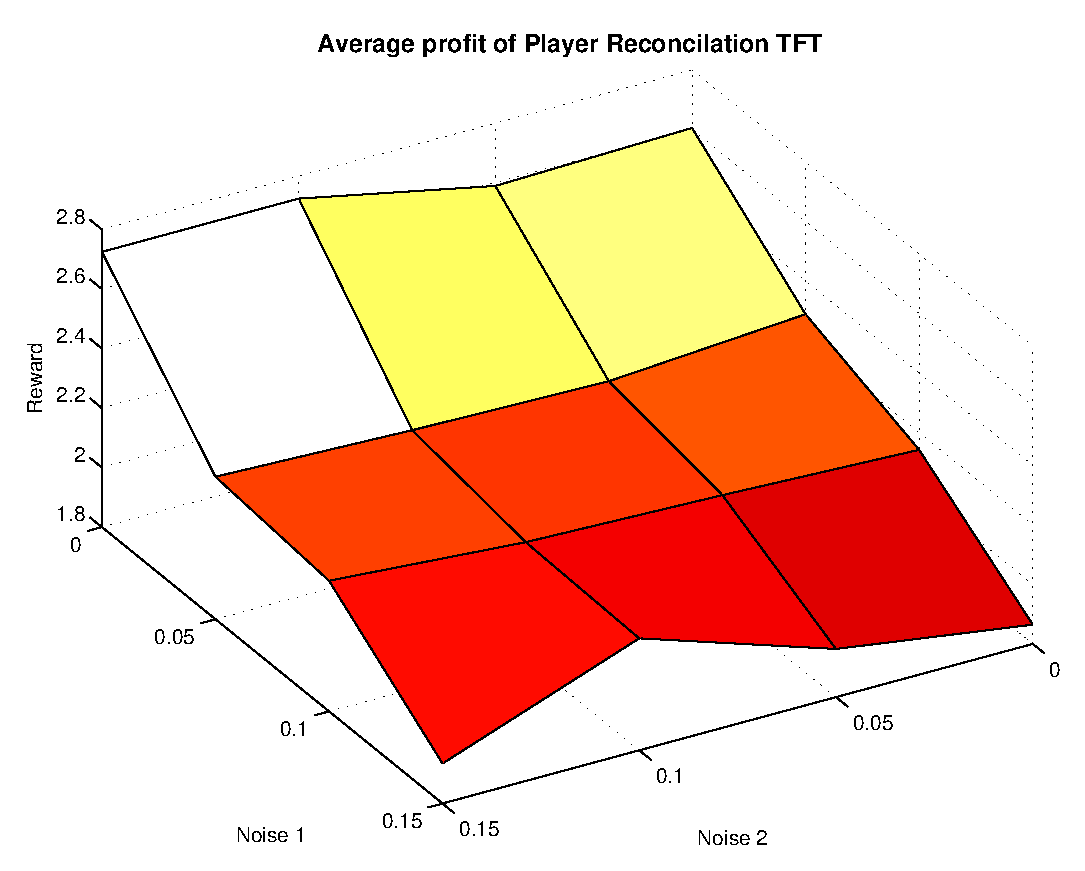
\includegraphics[width=\textwidth]{pics/simulation1/Reward_vs_Noise_of_Player_Reconcilation_TFT}
\end{minipage}
\hfill
\begin{minipage}[hbt]{0.3\textwidth}
	\centering
	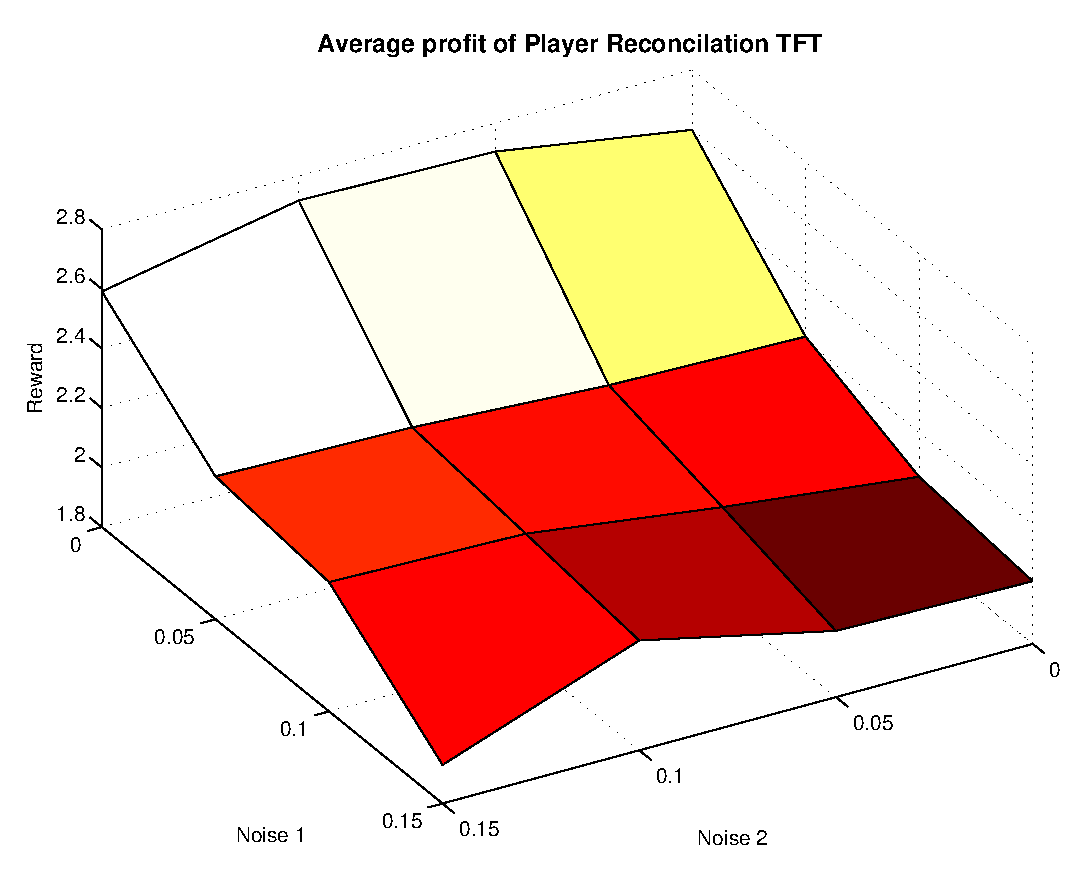
\includegraphics[width=\textwidth]{pics/simulation2/Reward_vs_Noise_of_Player_Reconcilation_TFT}
\end{minipage}
	\caption{Reward plot of the Player Reconciliation Tit For Tat}
	\label{pic player rtft}
\end{figure}

Like other more forgiving TFT mutants he has similar performance to TFT without noise, and drops less with noise1. The disadvantage of this player is that while it is not exploitable it still performs worse against defective players, when its reconciliation attempts are shut down over and over again.

\begin{table}[h]
 \begin{center}
\caption{Cooperation of Reconcilation Tit For Tat depending on the noise} \vspace{3mm}
\begin{tabular}{|l|c|c|c|c|c|}
\hline
   	& Noise 2 = 0 & Noise 2 = 0.05& Noise 2 = 0.1& Noise 2 = 0.15 \\
  \hline
  Noise 1 = 0 	&  0.8728  &  0.8972  &  0.9033 &   0.8723 \\
 \hline
  Noise 1 = 0.05	 &       0.7169 &   0.7218  &  0.7397 &   0.7450 \\
 \hline
  Noise 1 = 0.10 	&       0.6861 &   0.7010 &   0.7175  &  0.7217 \\
 \hline
  Noise 1 = 0.15 	&      0.6930 &   0.6955  &  0.7161  &  0.67528 \\
 \hline
\end{tabular}
 \end{center}
\end{table}

The number of cooperations is very high even with high noise1, at noise1=0.15 it's cooperation is higher than that of most TFT mutants. Generally the number of cooperative moves is more similar to Diekmann than to TFAT.

Traits different to TFT:

\renewcommand{\labelitemi}{}
\begin{itemize}
	\item + Initiates Cooperation
\end{itemize}
\renewcommand{\labelitemi}{$\bullet$}
 
\subsubsection{CDowning and DDowning}
The two players' performance in both simulations is shown in the two figures below:
\begin{figure}[h]
\begin{minipage}[hbt]{0.65\textwidth}
	\centering
	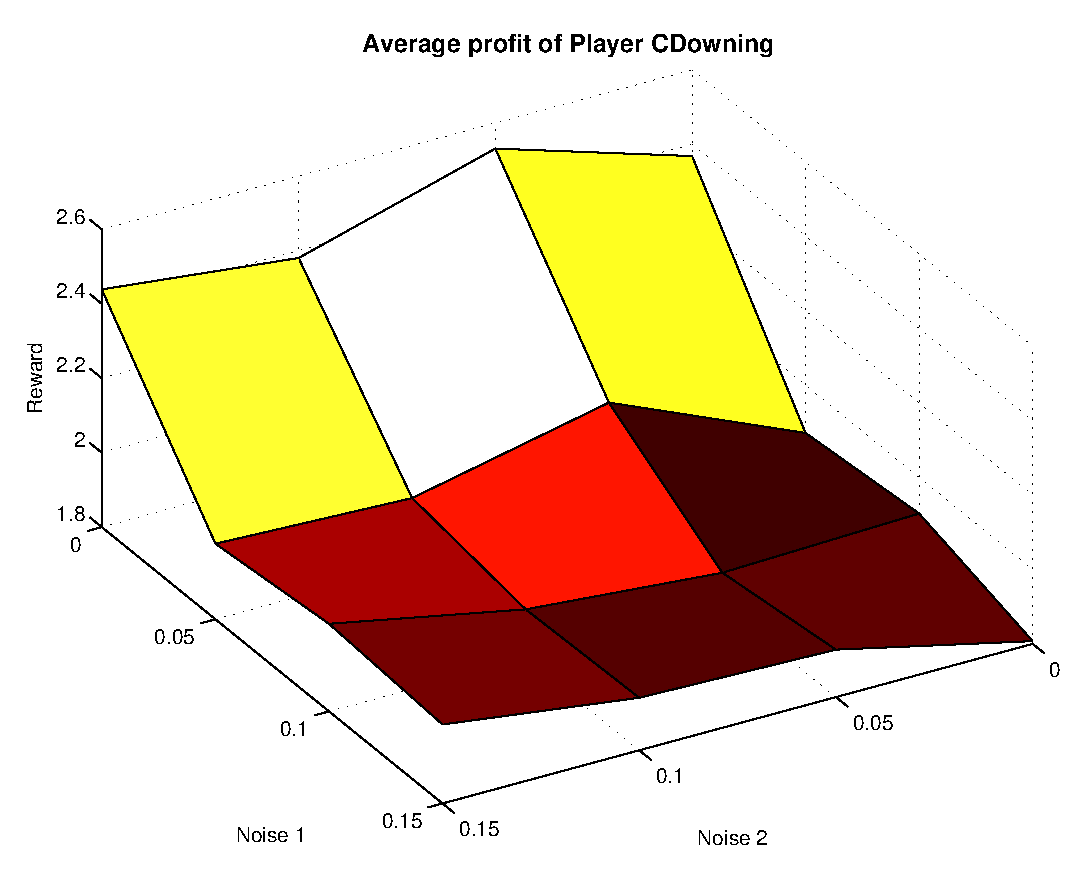
\includegraphics[width=\textwidth]{pics/simulation1/Reward_vs_Noise_of_Player_CDowning}
\end{minipage}
\hfill
\begin{minipage}[hbt]{0.3\textwidth}
	\centering
	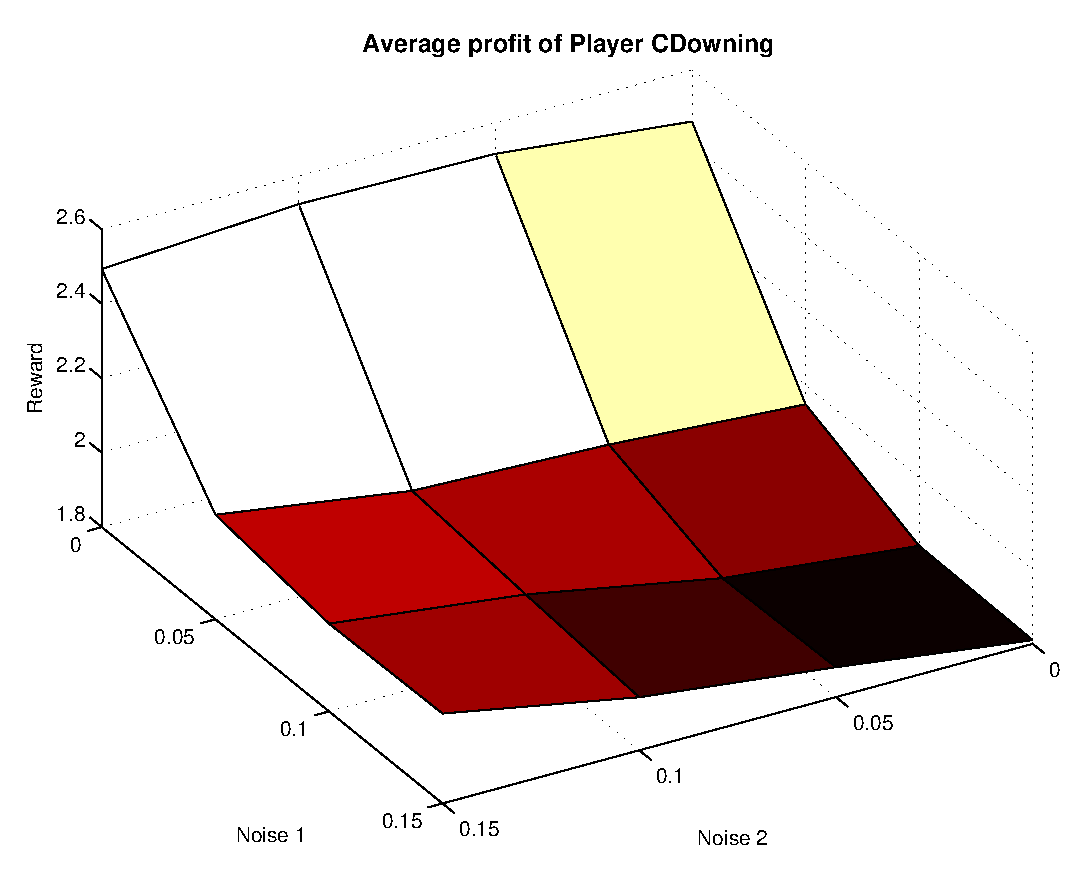
\includegraphics[width=\textwidth]{pics/simulation2/Reward_vs_Noise_of_Player_CDowning}
\end{minipage}
	\caption{Reward plot of the Player CDowning}
	\label{pic player cd}
\end{figure}

\begin{figure}[h]
\begin{minipage}[hbt]{0.65\textwidth}
	\centering
	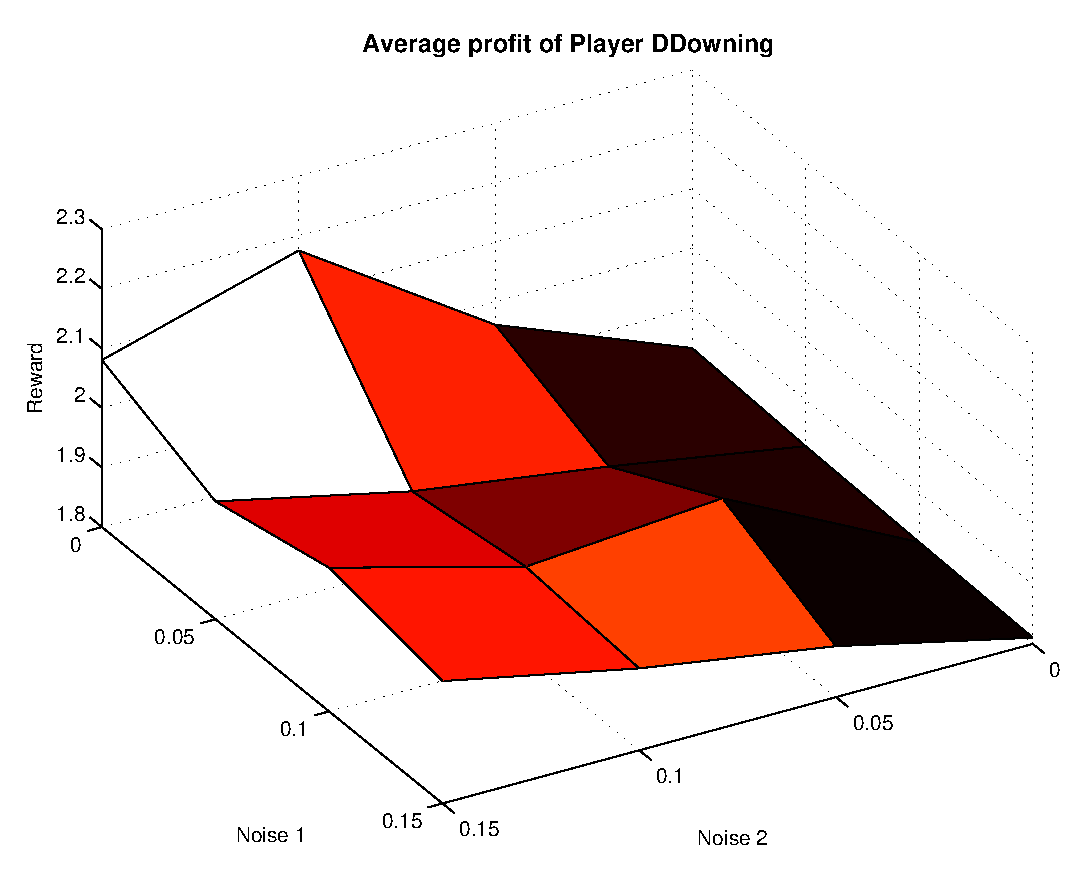
\includegraphics[width=\textwidth]{pics/simulation1/Reward_vs_Noise_of_Player_DDowning}
\end{minipage}
\hfill
\begin{minipage}[hbt]{0.3\textwidth}
	\centering
	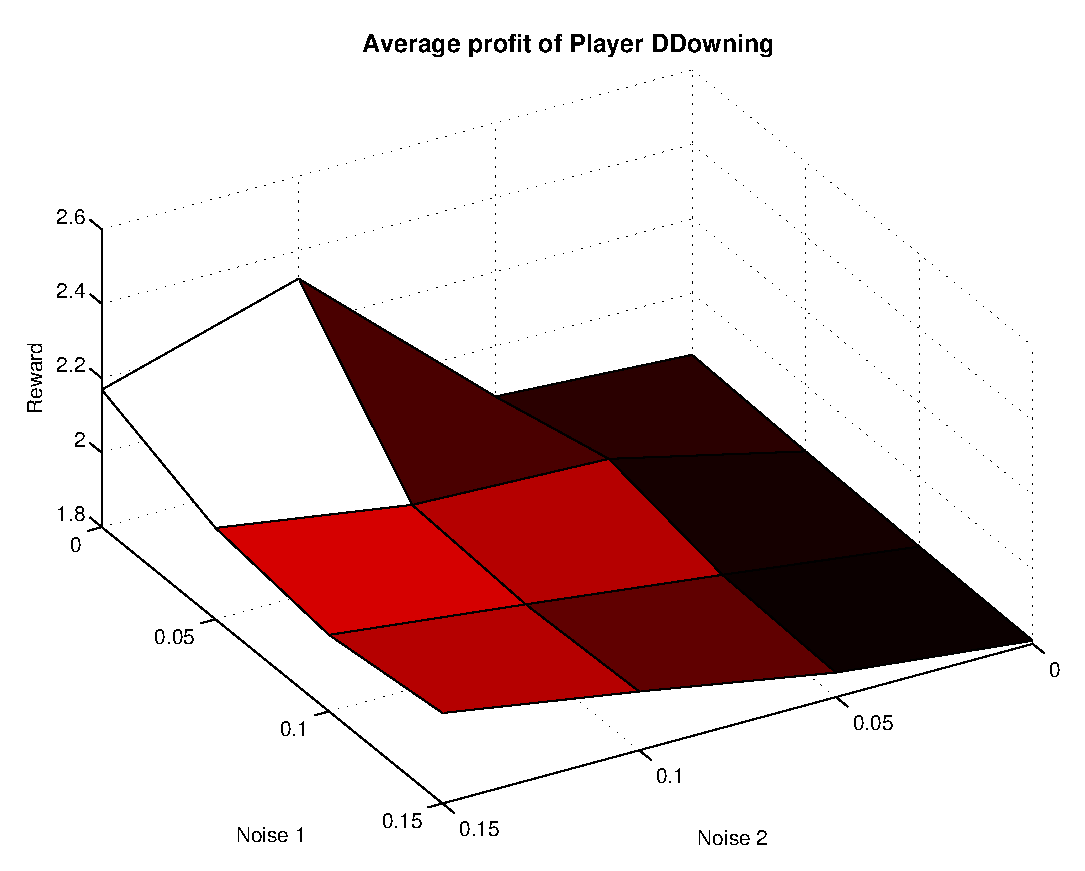
\includegraphics[width=\textwidth]{pics/simulation2/Reward_vs_Noise_of_Player_DDowning}
\end{minipage}
	\caption{Reward plot of the Player DDowning}
	\label{pic player dd}
\end{figure}

If Noise1 is zero, then CDownig performs stronger than DDowning. DDowning performs generally poorly with high Noise2 and no Noise1 there is a slight performance gain. At no noise DDowning outperforms CDowning against "Cooperate" and "Watcher", but is much worse against all TFT mutants and Friedmann. Noise2 improves the performance of DDowning against the TFT mutants a little. In the individual parings it seems that DDowning can end up in either mutual rejection or mutual cooperation. The decision where they end up seems to be random. For example at Noise2=0.15 mutual cooperation appears in TFT and TF2T, but not in Diekmann and Joss, while at Noise2=0.1 it is the other way around.

\begin{table}[h]
 \begin{center}
\caption{Cooperations of CDowning depending on the Noise} \vspace{3mm}
\begin{tabular}{|l|c|c|c|c|c|}
\hline
   	& Noise 2 = 0 & Noise 2 = 0.05& Noise 2 = 0.1& Noise 2 = 0.15 \\
  \hline
  Noise 1 = 0 	&      0.7507  &  0.6013 &   0.7660 &  0.6504 \\
 \hline
  Noise 1 = 0.05	 &           0.1210  &  0.1711  &  0.0829 &  0.0507 \\
 \hline
  Noise 1 = 0.10 	&          0.1169   & 0.0507 &   0.0508  &  0.0508 \\
 \hline
  Noise 1 = 0.15 	&        0.0507  &  0.0745 &   0.0504 &  0.0505 \\
 \hline
\end{tabular}
 \end{center}
\end{table}

\begin{table}[h]
 \begin{center}
\caption{Cooperations of CDowning depending on the Noise} \vspace{3mm}
\begin{tabular}{|l|c|c|c|c|c|}
\hline
   	& Noise 2 = 0 & Noise 2 = 0.05& Noise 2 = 0.1& Noise 2 = 0.15 \\
  \hline
  Noise 1 = 0 	&        0.0500  &  0.1499&   0.2997  &  0.3500 \\
 \hline
  Noise 1 = 0.05	 &              0.0500   & 0.0501  &  0.0517  & 0.0502 \\
 \hline
  Noise 1 = 0.10 	&             0.0500 &   0.1110  &  0.0503  &  0.0502 \\
 \hline
  Noise 1 = 0.15 	&          0.0501  &  0.0501 &   0.0501  &  0.0502 \\
 \hline
\end{tabular}
 \end{center}
\end{table}

DDowning seems to reject almost all the time, while CDowning rejects most of the time if Noise1 is greater than 0. A problem of Downing is that it compares decisions that hapen at the same time, but at this time the opponent does not know Downings decision, so his decision can only be dependant on Downings past decisions.
%%%%%

%%%%%
\newpage
\subsubsection{Tit For Tat with Reputation}
The player's performance in both simulations is shown in the two figures below:
\begin{figure}[h]

\begin{minipage}[hbt]{0.65\textwidth}
	\centering
	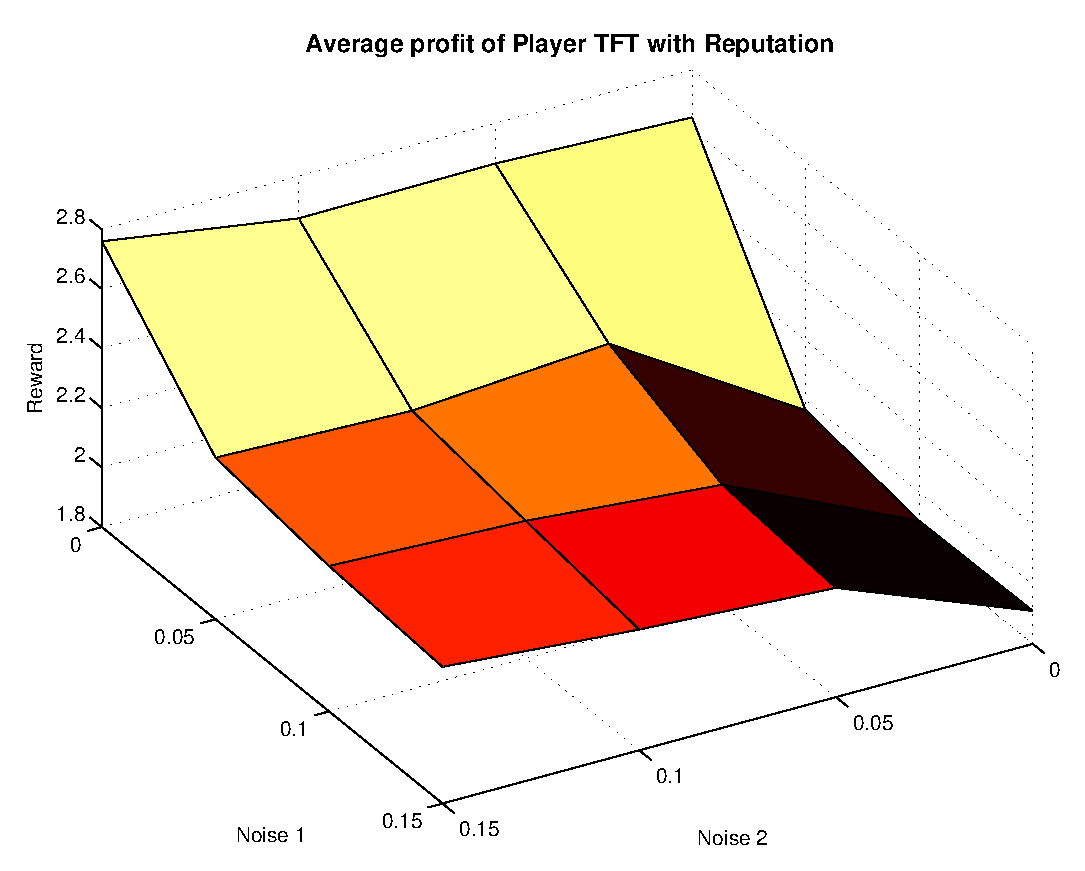
\includegraphics[width=\textwidth]{pics/simulation1/Reward_vs_Noise_of_Player_TFT_with_Reputation}
\end{minipage}
\hfill
\begin{minipage}[hbt]{0.3\textwidth}
	\centering
	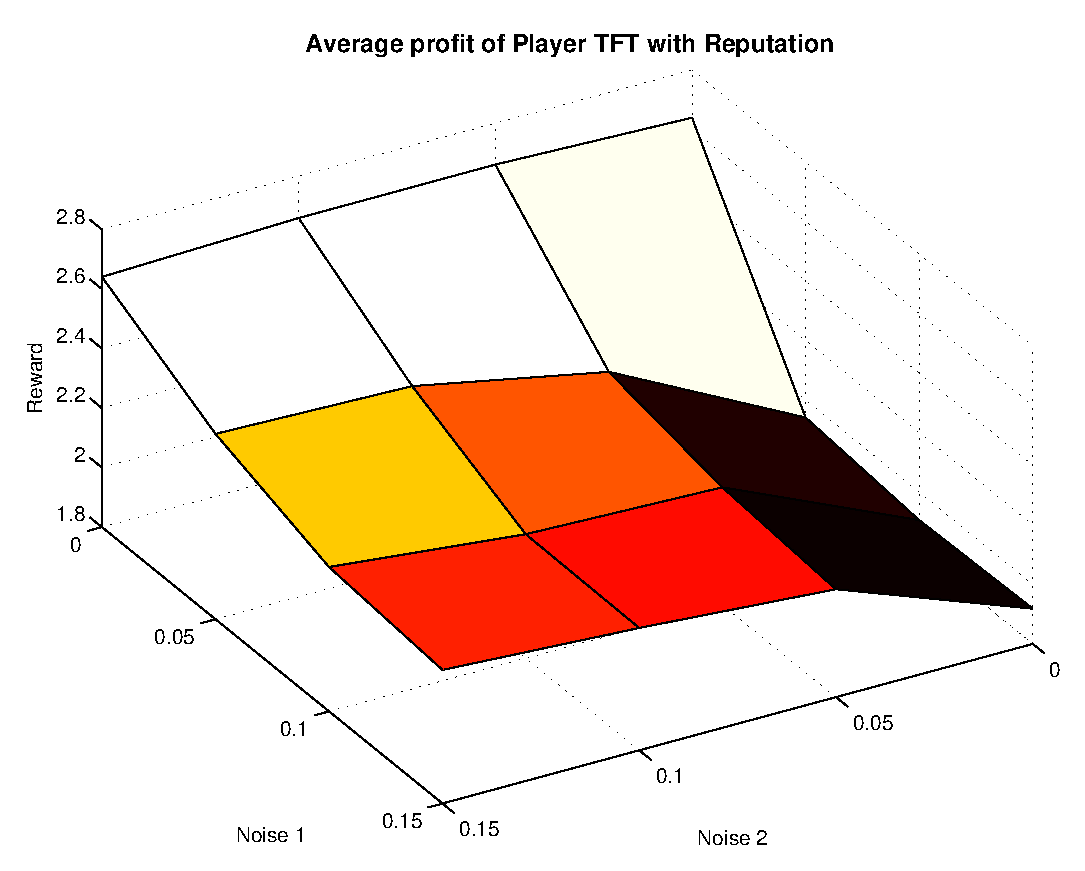
\includegraphics[width=\textwidth]{pics/simulation2/Reward_vs_Noise_of_Player_TFT_with_Reputation}
\end{minipage}
	\caption{Reward plot of the Player Tit For Tat with Reputation}
	\label{pic player tftwr}
\end{figure}

There were too many unfriendly players, that any player could have been friendly enough so that this player would have looked over a defection. The only player that would cooperate enough is "Cooperate". Against this player the number of cooperations was higher then the one of TFT, but because "Cooperate" is an exploitable player, this actually hurt this strategy.
In an environement where most players are cooperating this player could theoretically be exploited.

\begin{table}[h]
 \begin{center}
\caption{Cooperations of Tit For Tat with Reputation depending on the Noise} \vspace{3mm}
\begin{tabular}{|l|c|c|c|c|c|}
\hline
   	& Noise 2 = 0 & Noise 2 = 0.05& Noise 2 = 0.1& Noise 2 = 0.15 \\
  \hline
  Noise 1 = 0 	&           0.8059  & 0.8218&    0.8375   & 0.8440 \\
 \hline
  Noise 1 = 0.05	 &     0.8059  &  0.8218 &   0.8375   & 0.84402 \\
 \hline
  Noise 1 = 0.10 	&     0.3476  &  0.4939  &  0.5341  &  0.5942 \\
 \hline
  Noise 1 = 0.15 	&    0.3202 &   0.4402 &   0.4906 &   0.5349 \\
 \hline
\end{tabular}
 \end{center}
\end{table}

The values in the upper table are very similar to the results of Tit For Tat
%%%%%

%%%%%
\newpage
\subsubsection{Strategy Switcher}
The player's performance in both simulations is shown in the two figures below:
\begin{figure}[h]

\begin{minipage}[hbt]{0.65\textwidth}
	\centering
	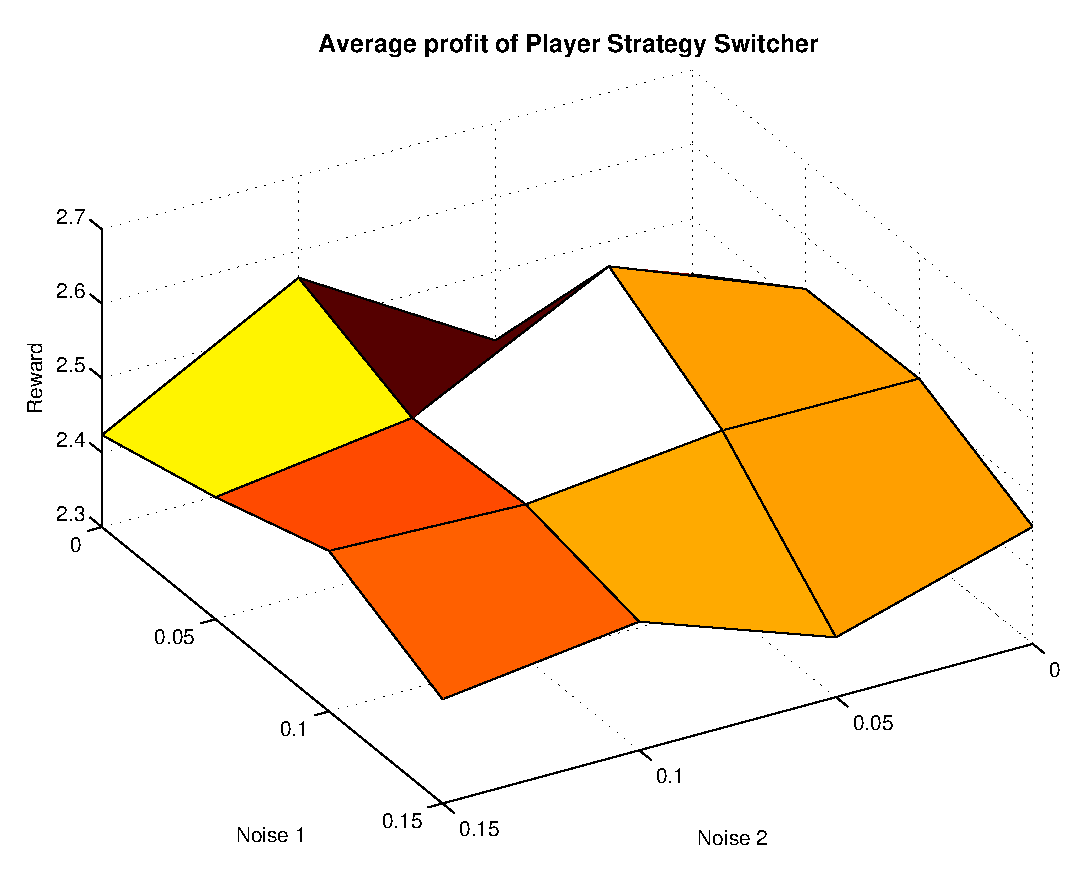
\includegraphics[width=\textwidth]{pics/simulation1/Reward_vs_Noise_of_Player_Strategy_Switcher}
\end{minipage}
\hfill
\begin{minipage}[hbt]{0.3\textwidth}
	\centering
	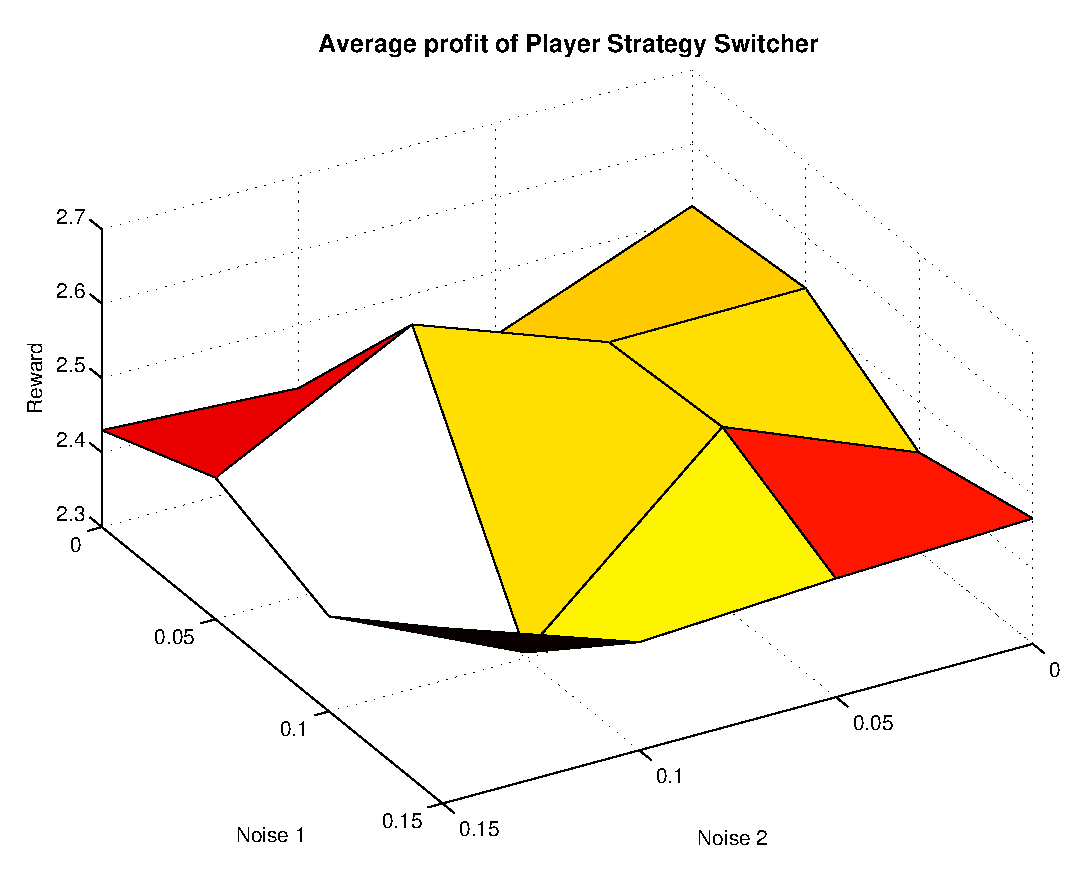
\includegraphics[width=\textwidth]{pics/simulation2/Reward_vs_Noise_of_Player_Strategy_Switcher}
\end{minipage}
	\caption{Reward plot of the Player Strategy Switcher}
	\label{pic player ss}
\end{figure}

This player was by far the strongest player before the Downing players were added to the simulation. In the final simulation he is strong in fields, where the Noise is large as is performance is not impacted by noise. The disadvantage comes from trying out different strategies in the beginning. In the case of no noise this means that Friedmann will always defect. In the case of Downing mutants this seems to result in defections from the Downing players. Before these Downing players were added this player outperformed TFt by a huge margin, even at zero noise. The strength of this player comes from his ability to cooperate with TFT mutants and exploit exploitable players. This player might even be stronger if better strategies were given to his arsenal. Currently he had "Cooperate", "Defect", TFT, TF2T and Pavlov as choices. A more efficient choice might have been Limited Reconciliation TFT and "Defect". Currently it also contains exploitable strategies (TF2T), so the player could be exploited.

In long simulations the player can benefit from having the optimal strategy, while in short simulations he spends a large amount of the time trying out strategies that might not be very strong.

\begin{table}[h]
 \begin{center}
\caption{Cooperations of Strategy Switcher depending on the Noise} \vspace{3mm}
\begin{tabular}{|l|c|c|c|c|c|}
\hline
   	& Noise 2 = 0 & Noise 2 = 0.05& Noise 2 = 0.1& Noise 2 = 0.15 \\
  \hline
  Noise 1 = 0 	&     0.5164 &   0.5430  &  0.4803  &  0.4659 \\
 \hline
  Noise 1 = 0.05	 &    0.5164  &  0.5430   & 0.4803   & 0.4659 \\
 \hline
  Noise 1 = 0.10 	&    0.5098  &  0.5520  &  0.4497 &   0.4888 \\
 \hline
  Noise 1 = 0.15 	&        0.5097  &  0.5318 &   0.4675 &   0.4467 \\
 \hline
\end{tabular}
 \end{center}
\end{table}

The number of cooperations is rather low, but also does not change very much with the noise. The number of cooperations is most likely low, because this player actively looks if an opponent is exploitable.

Traits of the player:


\renewcommand{\labelitemi}{}
\begin{itemize}
	\item + Can exploit others
	\item + Noise doesn't impact performance
	\item + Very adaptive
	\item + Strong in long simulations
	\item - Exploitable himself
	\item - Exploring defective moves can backfire (Friedmann)
	\item - Is hard to read initially, this might trigger defections
	\item - Weak in short simulations
\end{itemize}
\renewcommand{\labelitemi}{$\bullet$}
%%%%%

%%%%%
\newpage
\subsubsection{Lookback CDowning and Lookback DDowning}
The two players' performance in both simulations is shown in the two figures below:
\begin{figure}[h]

\begin{minipage}[hbt]{0.65\textwidth}
	\centering
	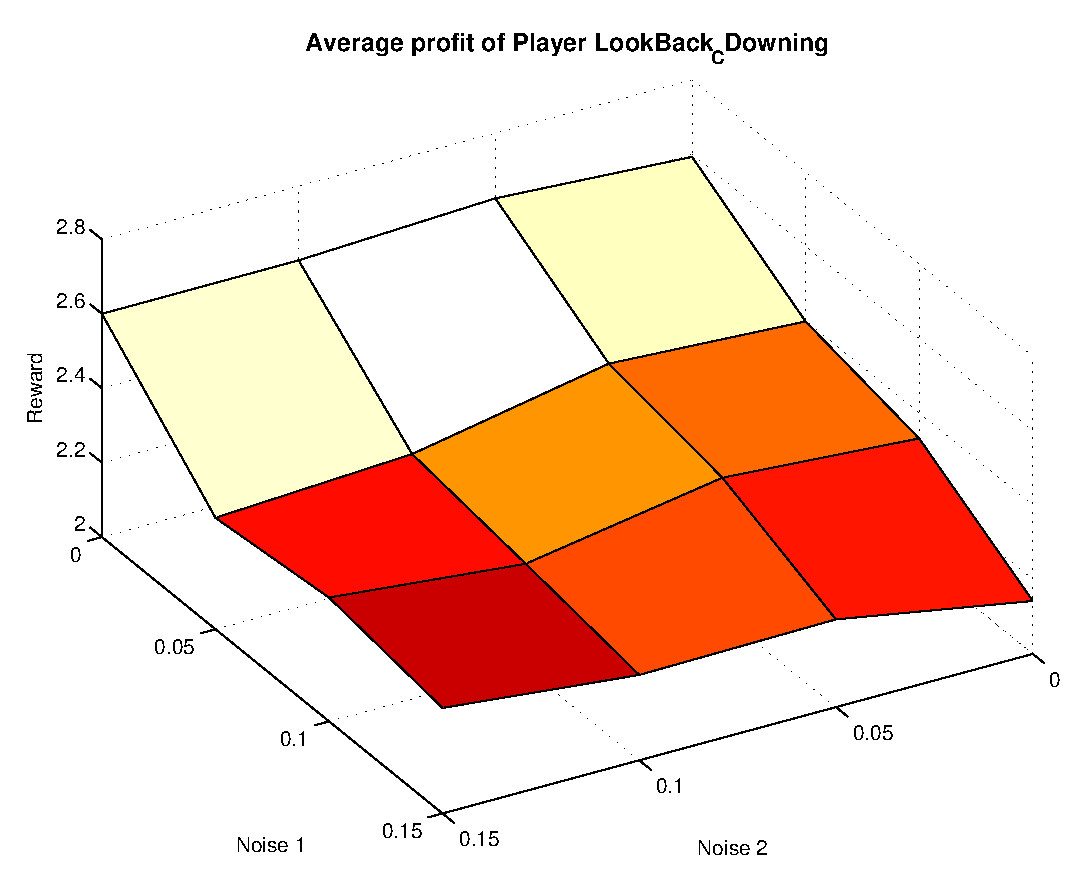
\includegraphics[width=\textwidth]{pics/simulation1/Reward_vs_Noise_of_Player_LookBack_CDowning}
\end{minipage}
\hfill
\begin{minipage}[hbt]{0.3\textwidth}
	\centering
	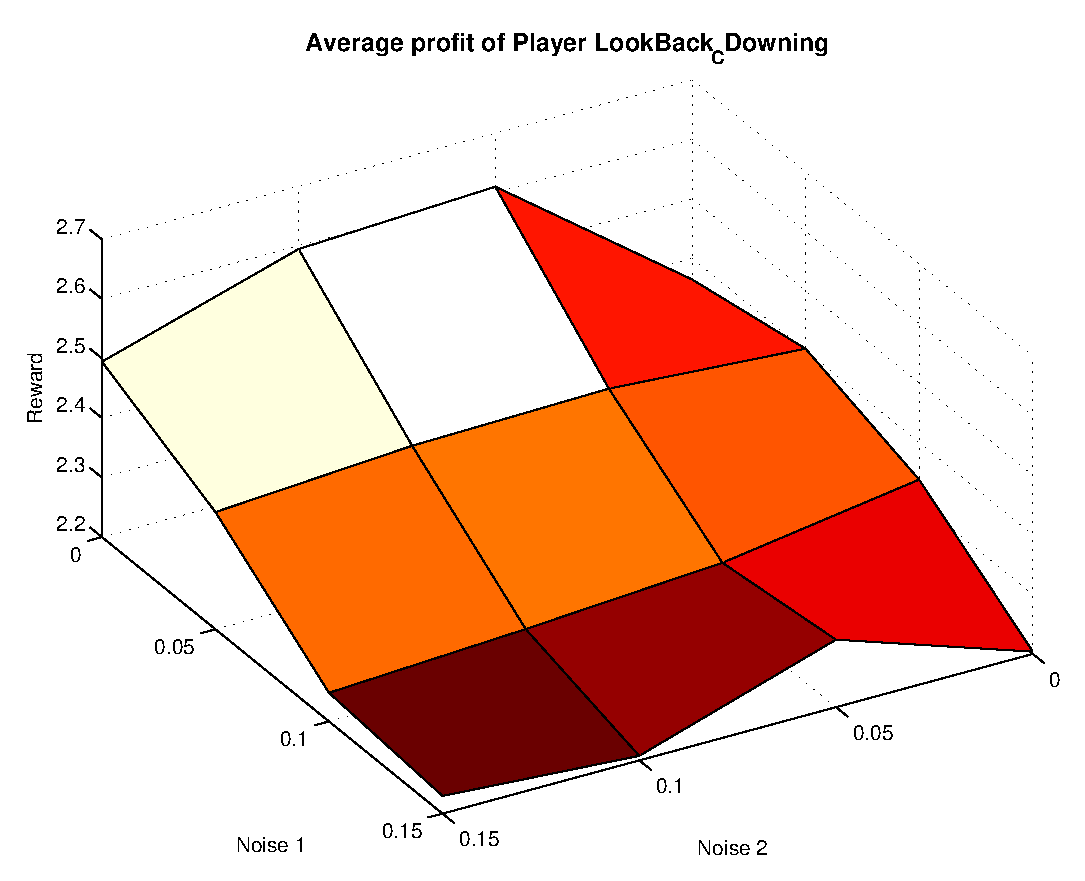
\includegraphics[width=\textwidth]{pics/simulation2/Reward_vs_Noise_of_Player_LookBack_CDowning}
\end{minipage}
	\caption{Reward plot of the Player Lookback CDowning}
	\label{pic player lbcd}
\end{figure}

\begin{figure}[h]

\begin{minipage}[hbt]{0.65\textwidth}
	\centering
	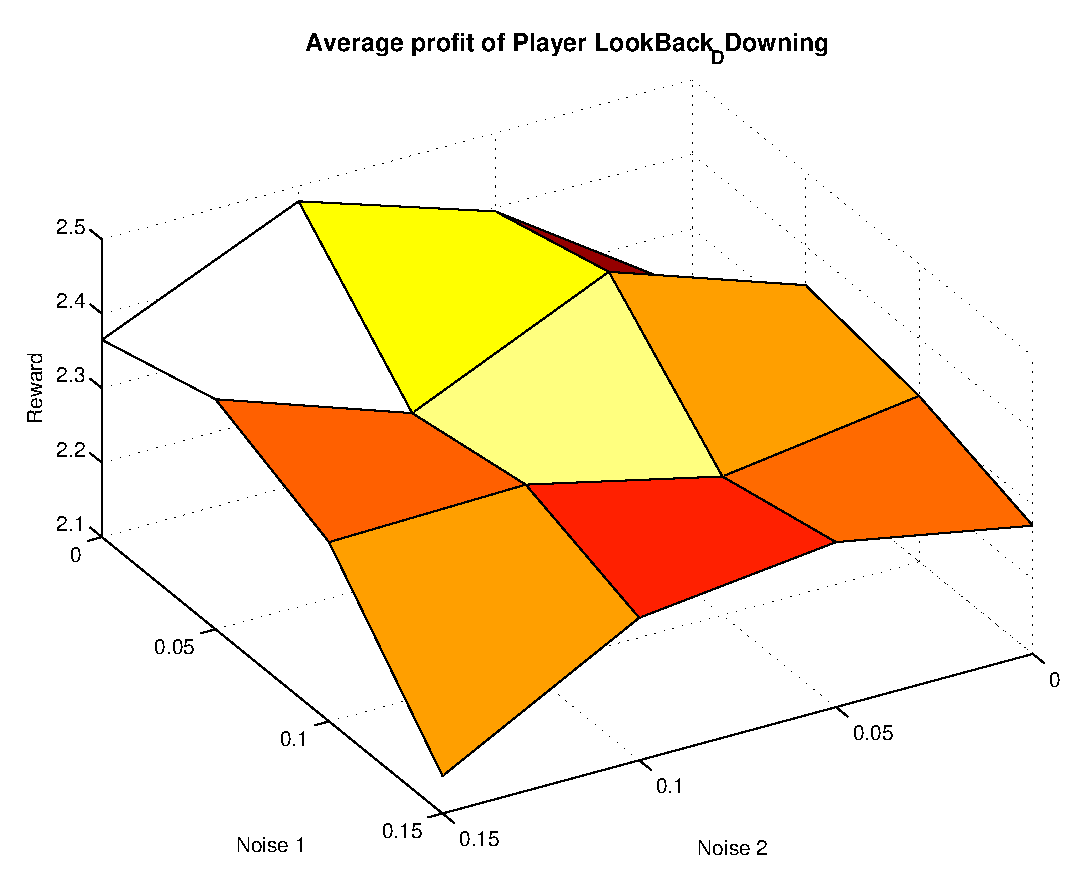
\includegraphics[width=\textwidth]{pics/simulation1/Reward_vs_Noise_of_Player_LookBack_DDowning}
\end{minipage}
\hfill
\begin{minipage}[hbt]{0.3\textwidth}
	\centering
	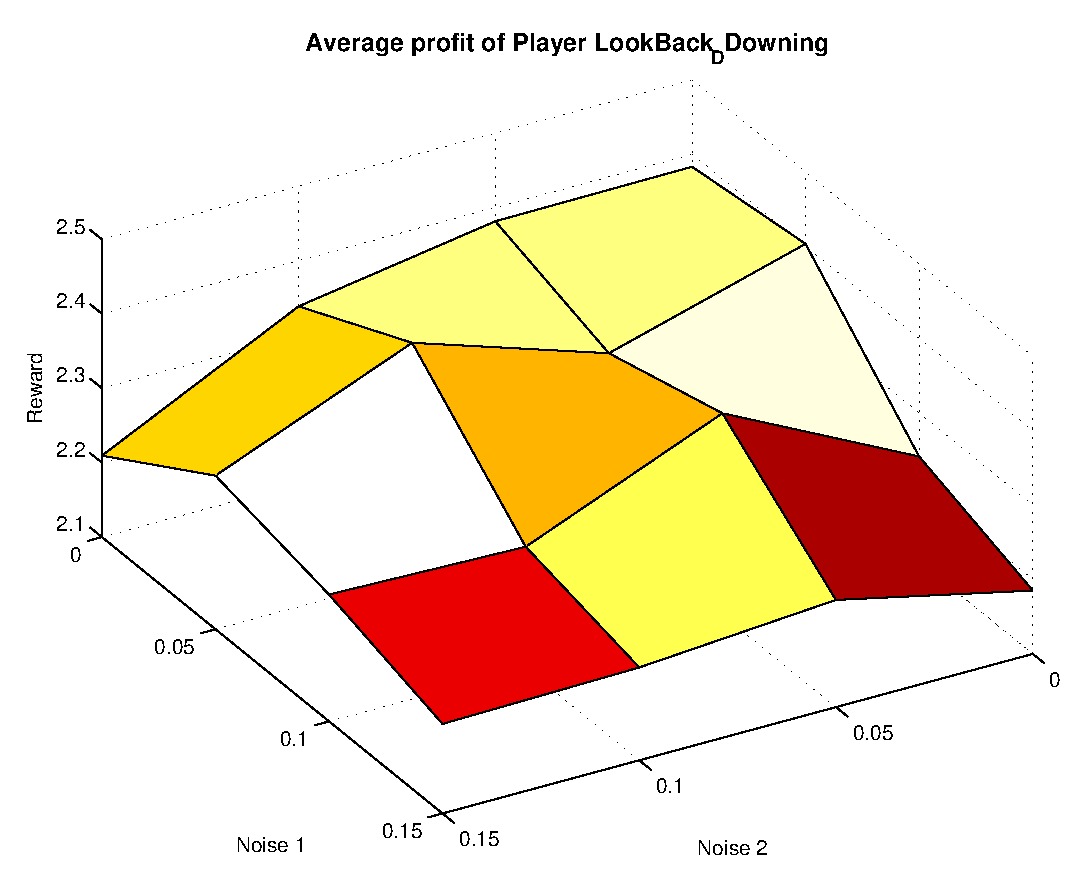
\includegraphics[width=\textwidth]{pics/simulation2/Reward_vs_Noise_of_Player_LookBack_DDowning}
\end{minipage}
	\caption{Reward plot of the Player Lookback DDowning}
	\label{pic player lbdd}
\end{figure}

Generally both Lookback Downings are stronger than the not Lookback Downings. If Noise1 is zero, the CDowning mutant has again a higher performance. Comparing the second last move with the last move of the opponent seems to be the better way to correlate your actions with your opponent's actions. DDowning seems to be very resilient to Noise.

At zero noise CDowning performs well with most players, except "Evolutionary", Strategy Switcher, and some Downing mutants. With noise the performance against Friedmann and some Downing mutants that went well before drops. The overall performance however stays higher than TFT. The Look-back Downing behaves similar like Lookback CDowning behaves with noise.

\begin{table}[h]
 \begin{center}
\caption{Cooperations of the Lookback CDowning depending on the Noise} \vspace{3mm}
\begin{tabular}{|l|c|c|c|c|c|}
\hline
   	& Noise 2 = 0 & Noise 2 = 0.05& Noise 2 = 0.1& Noise 2 = 0.15 \\
  \hline
  Noise 1 = 0 	&     0.7507   & 0.6511 &   0.6509&    0.7010 \\
 \hline
  Noise 1 = 0.05	 &      0.4385 &   0.4405 &   0.4376 &   0.4329 \\
 \hline
  Noise 1 = 0.10 	&      0.4297  &  0.3865  &  0.3787  &  0.3696 \\
 \hline
  Noise 1 = 0.15 	&    0.3814  &  0.4120 &   0.3682  &  0.3271 \\
 \hline
\end{tabular}
 \end{center}
\end{table}

\begin{table}[h]
 \begin{center}
\caption{Cooperations of the Lookback DDowning depending on the Noise} \vspace{3mm}
\begin{tabular}{|l|c|c|c|c|c|}
\hline
   	& Noise 2 = 0 & Noise 2 = 0.05& Noise 2 = 0.1& Noise 2 = 0.15 \\
  \hline
  Noise 1 = 0 	&   0.4037 &   0.4563 &   0.4071   & 0.4762 \\
 \hline
  Noise 1 = 0.05	 &     0.4386  &  0.3912 &   0.4303   & 0.3848 \\
 \hline
  Noise 1 = 0.10 	&      0.3864   & 0.4025  &  0.3784 &  0.3827 \\
 \hline
  Noise 1 = 0.15 	&    0.3868 &   0.3262 &   0.3840  &  0.3769 \\
 \hline
\end{tabular}
 \end{center}
\end{table}

The number of Cooperations is in general much higher then for the Variants that do not look-back. For Noise1 greater than zero about 40\% cooperative moves remain, while CDowning and DDowning fall down to 5-10\% cooperative moves. The average rewards for these players are also 0.2-0.5 higher then their not look-back counterparts.
%%%%%

%%%%%
\newpage
\subsubsection{Watcher}
The player's performance in both simulations is shown in the two figures below:
\begin{figure}[h]

\begin{minipage}[hbt]{0.65\textwidth}
	\centering
	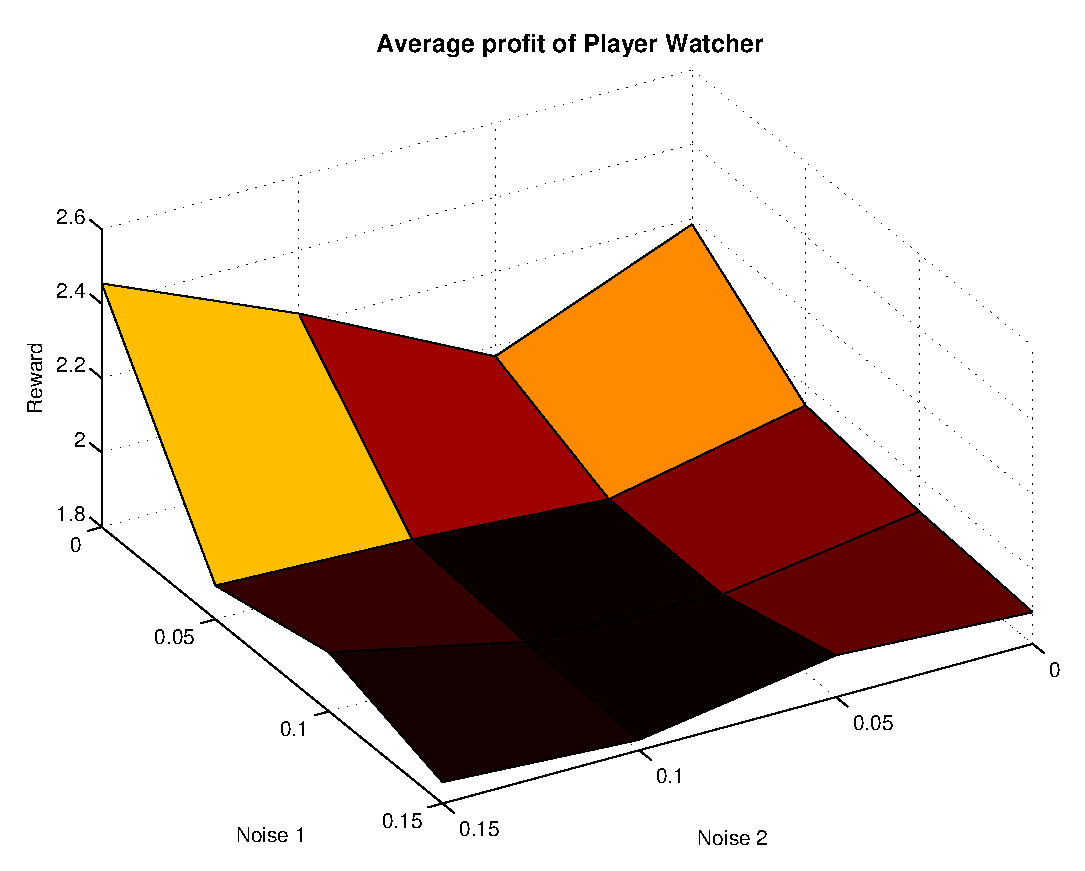
\includegraphics[width=\textwidth]{pics/simulation1/Reward_vs_Noise_of_Player_Watcher}
\end{minipage}
\hfill
\begin{minipage}[hbt]{0.3\textwidth}
	\centering
	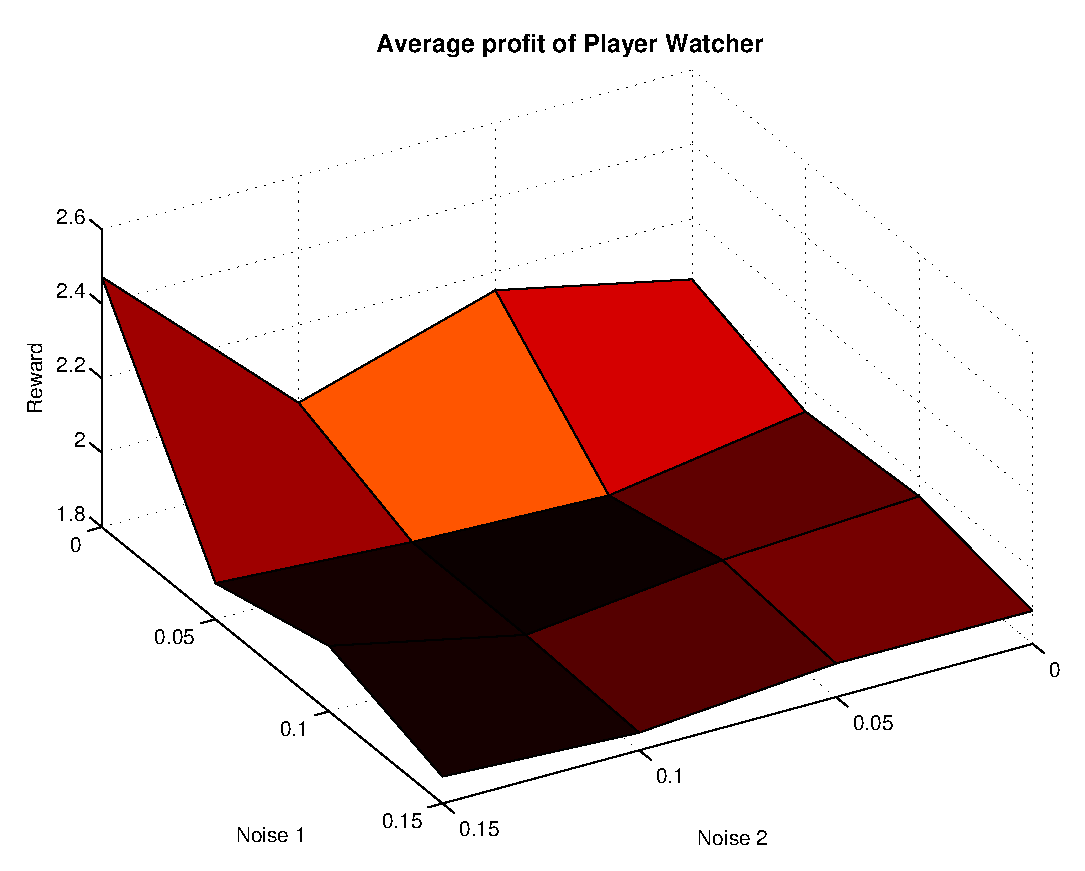
\includegraphics[width=\textwidth]{pics/simulation2/Reward_vs_Noise_of_Player_Watcher}
\end{minipage}
	\caption{Reward plot of the Player Watcher}
	\label{pic player watcher}
\end{figure}

This player generally does not perform very strong. It does not respond and can therefore be exploited. It also does not take the local situation into account. It will betray Friedmann even in no Noise, because in short term this is successful. After that the player copies strategies that were cooperative the whole time, while Friedmann is defecting. There is point of higher performance, where Noise2 is 0.15 and Noise 1 is zero. For some reason it performs strong against the Lookback-Downing algorithms.

\begin{table}[h]
 \begin{center}
\caption{Cooperations of the Watcher depending on the Noise} \vspace{3mm}
\begin{tabular}{|l|c|c|c|c|c|}
\hline
   	& Noise 2 = 0 & Noise 2 = 0.05& Noise 2 = 0.1& Noise 2 = 0.15 \\
  \hline
  Noise 1 = 0 	&       0.5399  &  0.4704  &  0.4298 &   0.4020 \\
 \hline
  Noise 1 = 0.05	 &        0.4569  &  0.3854 &   0.3544  & 0.3552 \\
 \hline
  Noise 1 = 0.10 	&         0.4297 &   0.3691  &  0.3522  &  0.3576 \\
 \hline
  Noise 1 = 0.15 	&       0.4125 &   0.3510&    0.3428  &  0.3504 \\
 \hline
\end{tabular}
 \end{center}
\end{table}

Generally the number of cooperations is rather low, but there are no drastic jumps.

%%%%%

%%%%%
\newpage
\subsubsection{Evolutionary}
The player's performance in both simulations is shown in the two figures below:
\begin{figure}[h]

\begin{minipage}[hbt]{0.65\textwidth}
	\centering
	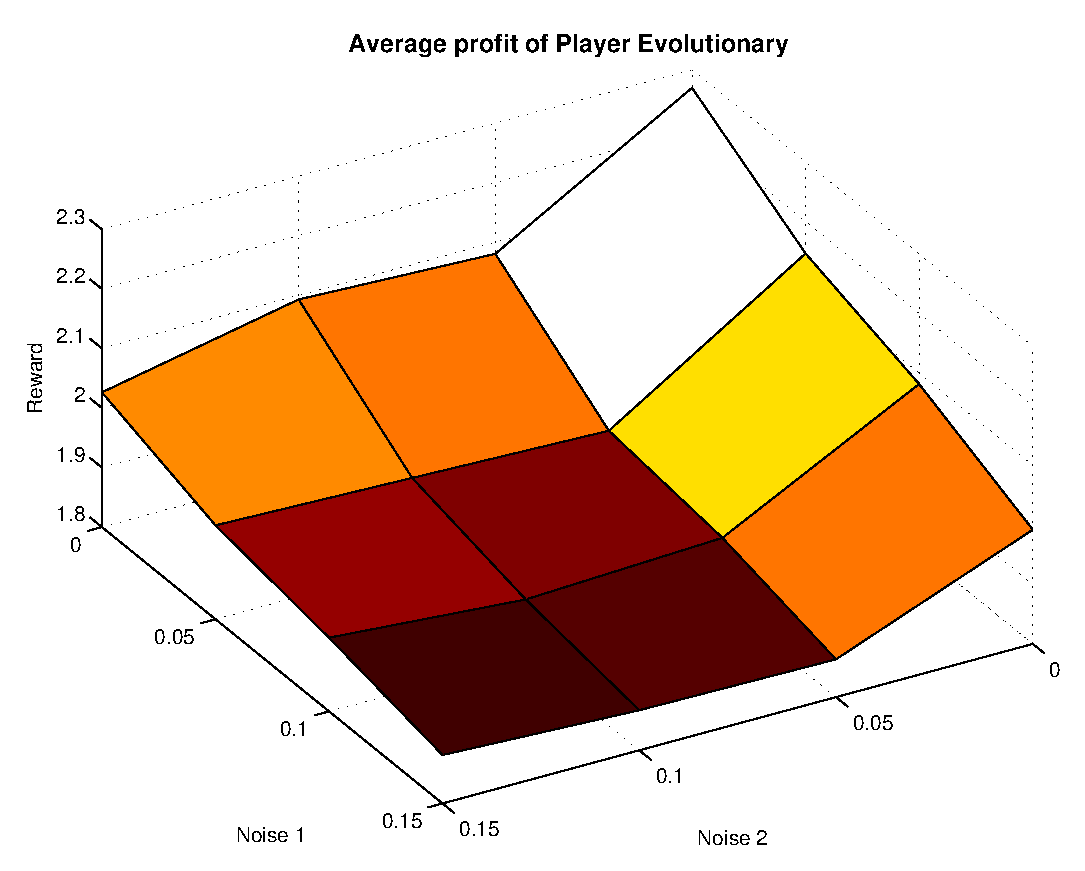
\includegraphics[width=\textwidth]{pics/simulation1/Reward_vs_Noise_of_Player_Evolutionary}
\end{minipage}
\hfill
\begin{minipage}[hbt]{0.3\textwidth}
	\centering
	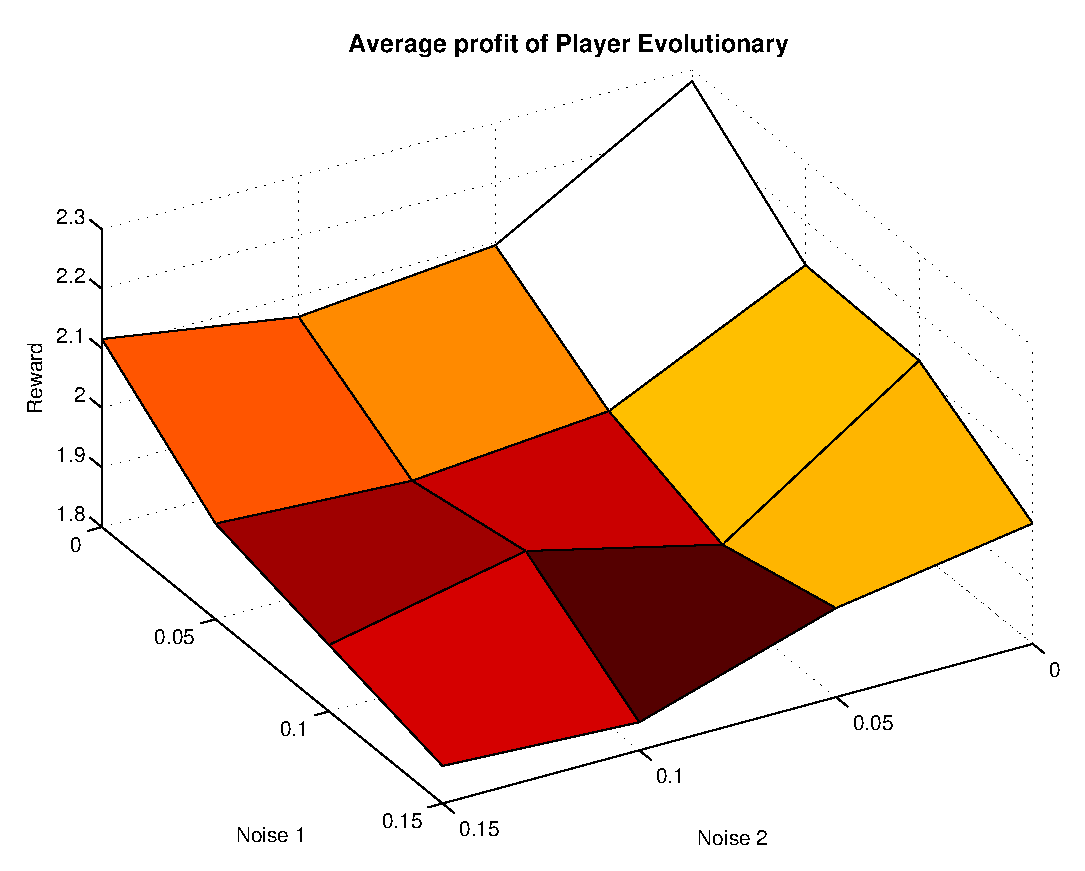
\includegraphics[width=\textwidth]{pics/simulation2/Reward_vs_Noise_of_Player_Evolutionary}
\end{minipage}
	\caption{Reward plot of the Player Evolutionary}
	\label{pic player evo}
\end{figure}

This player performs rather poorly at all noises. Less Noise is better for him, because more reliable information allows the player to adjust. Noise generally promotes bad strategies, while they are sorted out when there is little noise. The problem is that this players does add rejections and therefore triggers others rejections. The player himself has a very slow reaction time. Changing his strategy by mutations takes hundreds of turns. This is a stimescale the opponents cannot see. To the opponents this player does not look responsive. The player himself can only see the opponents reaction if it is within the segment legnth that the player tries to optimize. The interesting thing is that this player is able to exploit TF2T, he will add defections with mostly one sometimes two cooperative steps between them. It has a performance of 3.65 against TF2T at zero noise.

\begin{table}[h]
 \begin{center}
\caption{Cooperations of the Evolutionary depending on the Noise} \vspace{3mm}
\begin{tabular}{|l|c|c|c|c|c|}
\hline
   	& Noise 2 = 0 & Noise 2 = 0.05& Noise 2 = 0.1& Noise 2 = 0.15 \\
  \hline
  Noise 1 = 0 	&         0.4330 & 0.4941  &  0.5151  &  0.4878 \\
 \hline
  Noise 1 = 0.05	 &          0.3859   & 0.4745 &   0.4860 &   0.4855\\
 \hline
  Noise 1 = 0.10 	&    0.3987 &   0.4750&    0.4919&    0.4914 \\
 \hline
  Noise 1 = 0.15 	&     0.3755 &   0.4793  &  0.4733  &  0.4896 \\
 \hline
\end{tabular}
 \end{center}
\end{table}

The decisions seem to be mostly an even mix of defections and cooperations, with a slight preference of defections.

%%%%%

%%%%%
\newpage
\subsubsection{Limited Reconciliation Tit For tat}
The player's performance in both simulations is shown in the two figures below:
\begin{figure}[h]

\begin{minipage}[hbt]{0.65\textwidth}
	\centering
	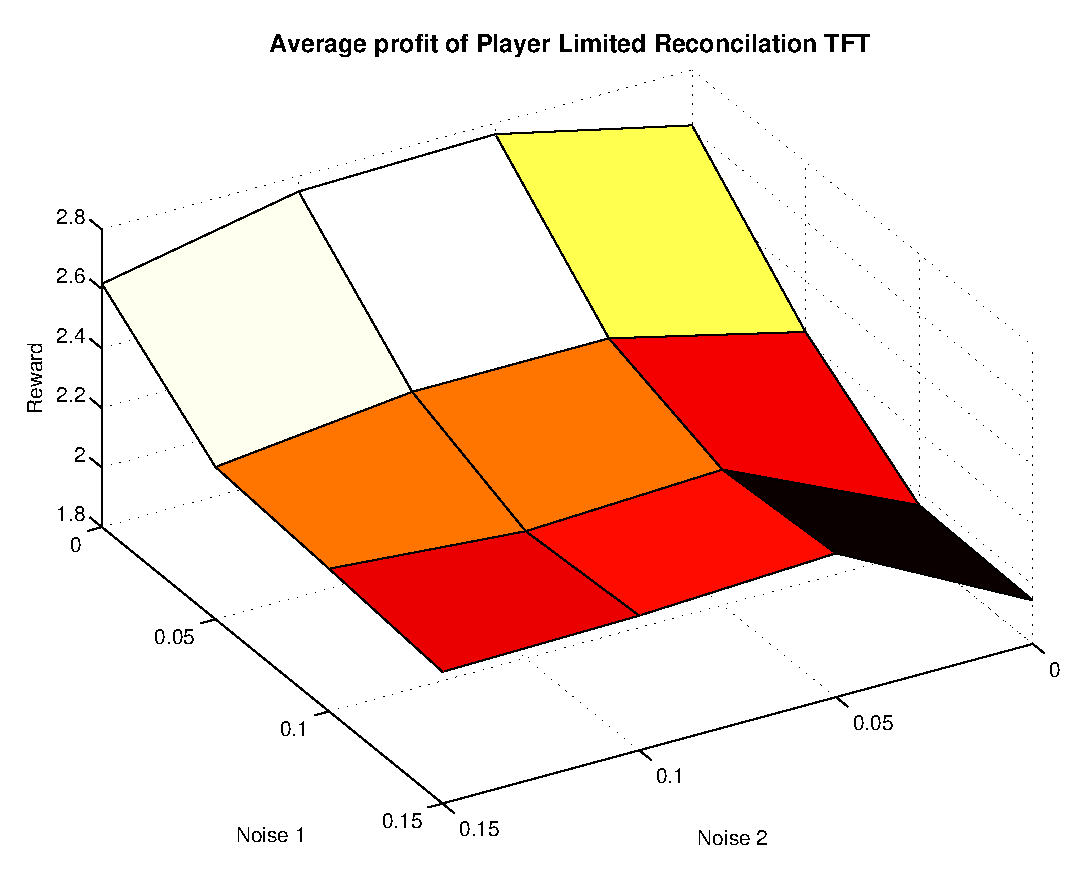
\includegraphics[width=\textwidth]{pics/simulation1/Reward_vs_Noise_of_Player_Limited_Reconcilation_TFT}
\end{minipage}
\hfill
\begin{minipage}[hbt]{0.3\textwidth}
	\centering
	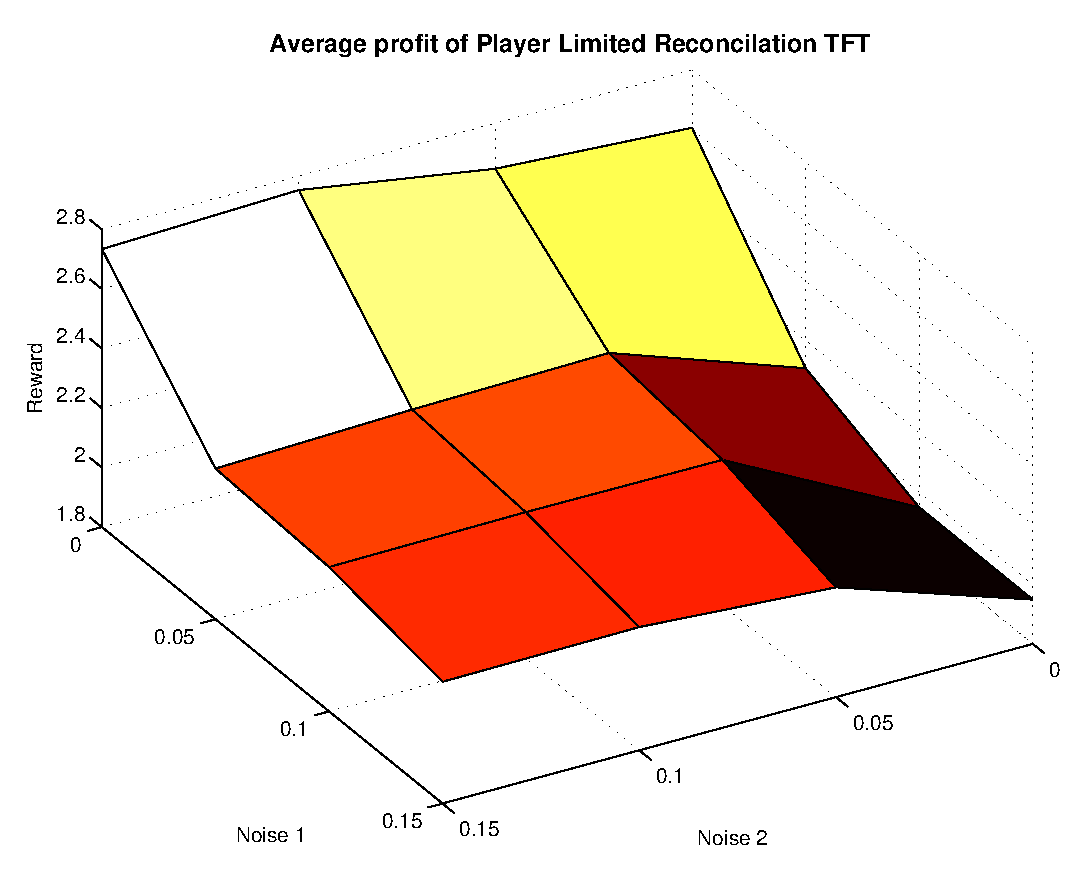
\includegraphics[width=\textwidth]{pics/simulation2/Reward_vs_Noise_of_Player_Limited_Reconcilation_TFT}
\end{minipage}
	\caption{Reward plot of the Player Limited Reconcilation Tit For tat}
	\label{pic player lrtft}
\end{figure}

At noise1 equal to zero the performance is similar to TFT. It does not perform as well as Reconciliation TFT against Joss, therefore it might be wiser to make the time between the reconciliation attempts larger every time, instead of limiting it to 3. Compared to TFT its performance does not break down that much with noise1, this is a property it shares with Diekmann, TFAT and Reconciliation TFT. The fact that the number of reconciliation attempts is limited makes the player stronger against defecting players like Friedmann (under noise1) and "Defect".


\begin{table}[h]
 \begin{center}
\caption{Cooperations of the Evolutionary depending on the Noise} \vspace{3mm}
\begin{tabular}{|l|c|c|c|c|c|}
\hline
   	& Noise 2 = 0 & Noise 2 = 0.05& Noise 2 = 0.1& Noise 2 = 0.15 \\
  \hline
  Noise 1 = 0 	&     0.8064&    0.8386 &   0.8942    &0.8976 \\
 \hline
  Noise 1 = 0.05	 &    0.5084  &  0.6577&    0.6834  &  0.7043\\
 \hline
  Noise 1 = 0.10 	&0.4254  &  0.6300 &   0.6568 &   0.6822 \\
 \hline
  Noise 1 = 0.15 	&    0.4208   & 0.5956  &  0.6383  &  0.6648 \\
 \hline
\end{tabular}
 \end{center}
\end{table}

It is not as cooperative as the friendliest TFT mutants Diekmann and RTFT, but more friendly than standard TFT and TFAT.

The table below shows the performance of LTFT minus the performance of TFT averaged over all matchups and both simulations:

\begin{table}[h]
 \begin{center}
\caption{Comparison of the two players Limited Tit Fot Tat and Tit For Tat} \vspace{3mm}
\begin{tabular}{|l|c|c|c|c|c|}
\hline
   	& Noise 2 = 0 & Noise 2 = 0.05& Noise 2 = 0.1& Noise 2 = 0.15 \\
  \hline
  Noise 1 = 0 	&    -0.0317 &   0.0414 &   0.0375&   -0.0892 \\
 \hline
  Noise 1 = 0.05	 &    0.2235 &  -0.0006  &  0.0310  & -0.0679\\
 \hline
  Noise 1 = 0.10 	&     0.0438&    0.0340  &  0.0019  &  0.0066 \\
 \hline
  Noise 1 = 0.15 	&     0.0514  &  0.0720  &  0.0189 &  -0.0312 \\
 \hline
\end{tabular}
 \end{center}
\end{table}

At higher values for Noise1, LTFT outperforms TFT, while at high Noise2 values the reconciliation attempts are not needed, because the noise itself achieves that.

\subsection{Impact of Noise on the whole system}

Below are the figures that show how the average Reward and the average Cooperation behave in the system.
Total Cooperation against Noise:

\begin{figure}[h]

\begin{minipage}[hbt]{0.65\textwidth}
	\centering
	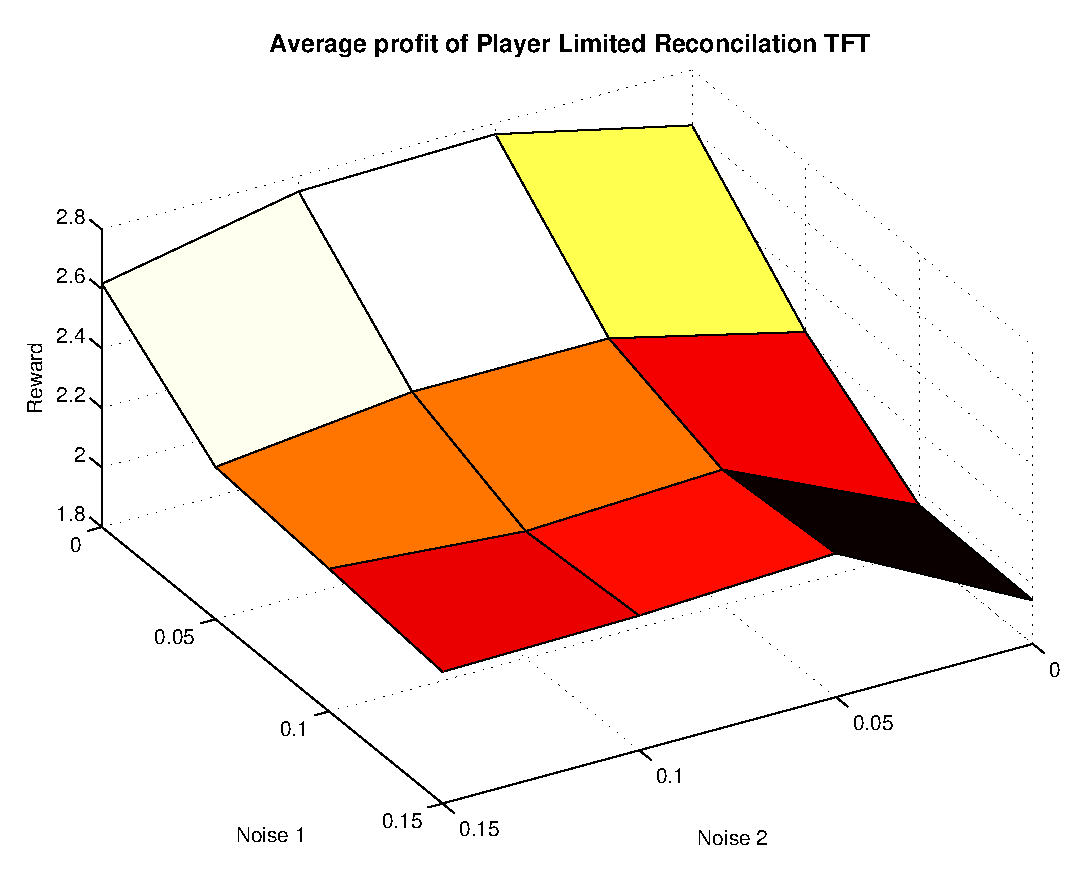
\includegraphics[width=\textwidth]{pics/simulation1/Reward_vs_Noise_of_Player_Limited_Reconcilation_TFT}
\end{minipage}
\hfill
\begin{minipage}[hbt]{0.3\textwidth}
	\centering
	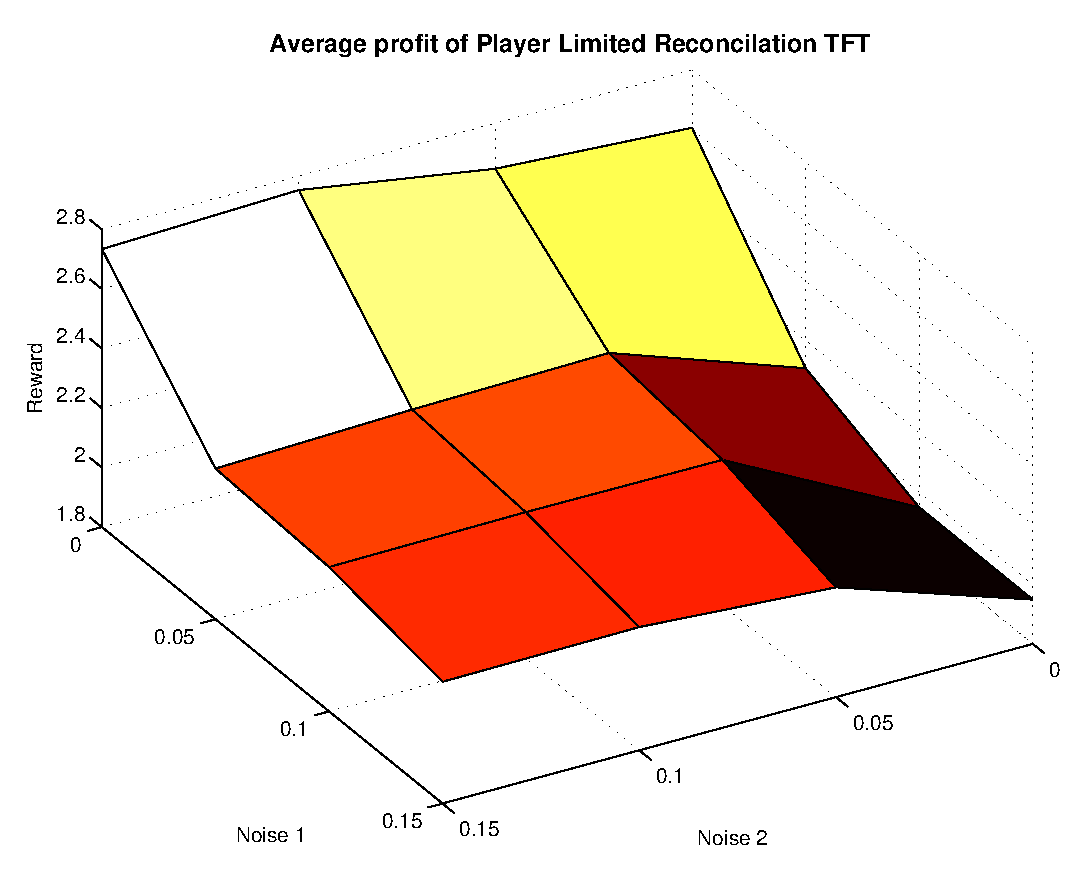
\includegraphics[width=\textwidth]{pics/simulation2/Reward_vs_Noise_of_Player_Limited_Reconcilation_TFT}
\end{minipage}
	\caption{Reward plot of the Player Limited Reconcilation Tit For tat}
	\label{pic player lrtft}
\end{figure}

Average Reward against Noise

\begin{figure}[h]

\begin{minipage}[hbt]{0.65\textwidth}
	\centering
	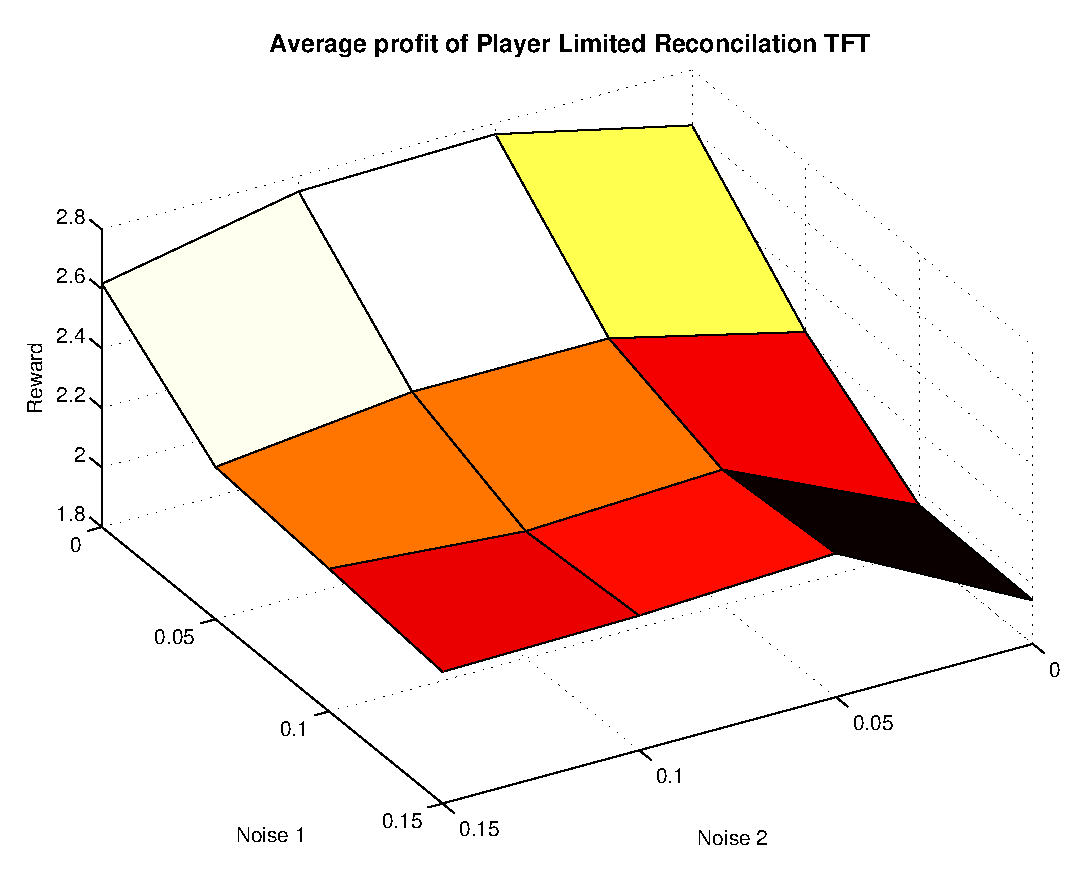
\includegraphics[width=\textwidth]{pics/simulation1/Reward_vs_Noise_of_Player_Limited_Reconcilation_TFT}
\end{minipage}
\hfill
\begin{minipage}[hbt]{0.3\textwidth}
	\centering
	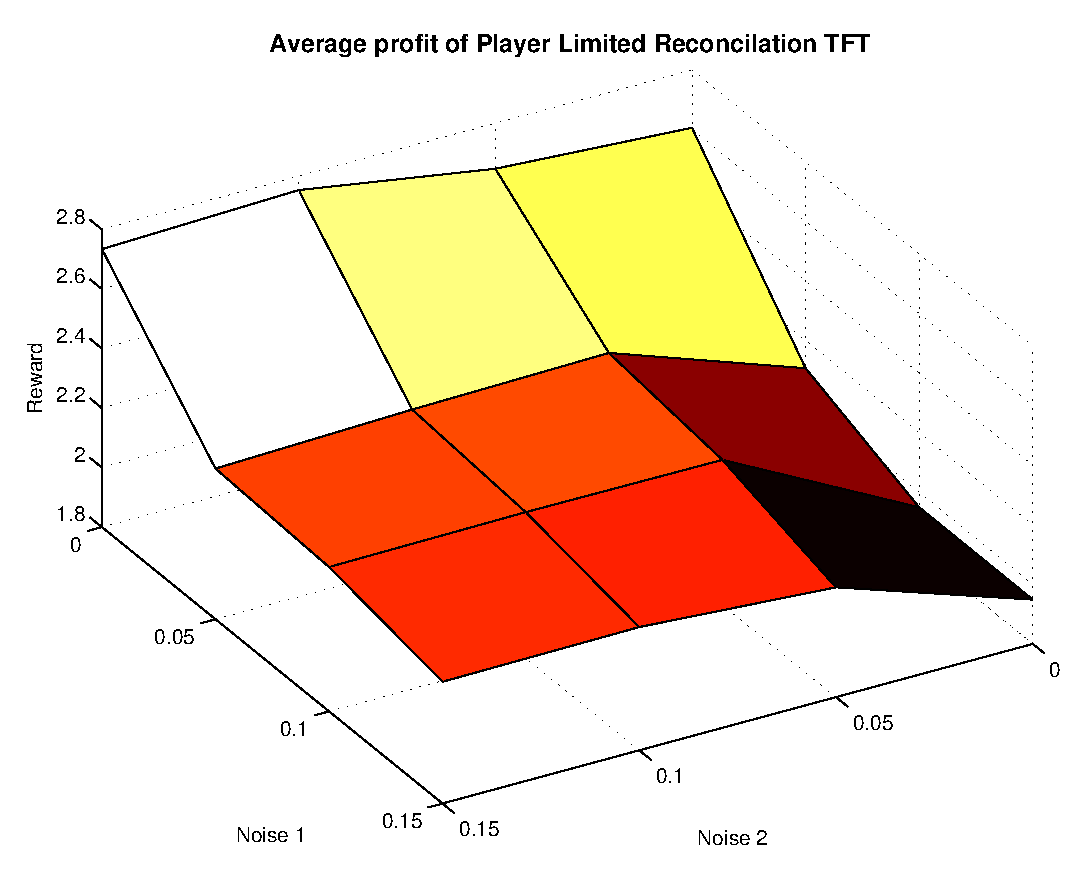
\includegraphics[width=\textwidth]{pics/simulation2/Reward_vs_Noise_of_Player_Limited_Reconcilation_TFT}
\end{minipage}
	\caption{Reward plot of the Player Limited Reconcilation Tit For tat}
	\label{pic player lrtft}
\end{figure}


Noise 1 seems to destroy cooperation really fast, while Noise2 increases it a little. Generally the average reward is the highest if the number of cooperative moves is the highest. The Average Rewards dependence on the noise looks very similar to the values a typical TFT mutant has. This may be related to the fact, that there were 8 TFT mutants in the simulation.

\subsection{Comparison of the players}

Best strategy at each Noise:

\begin{figure}[h]

\begin{minipage}[hbt]{0.65\textwidth}
	\centering
	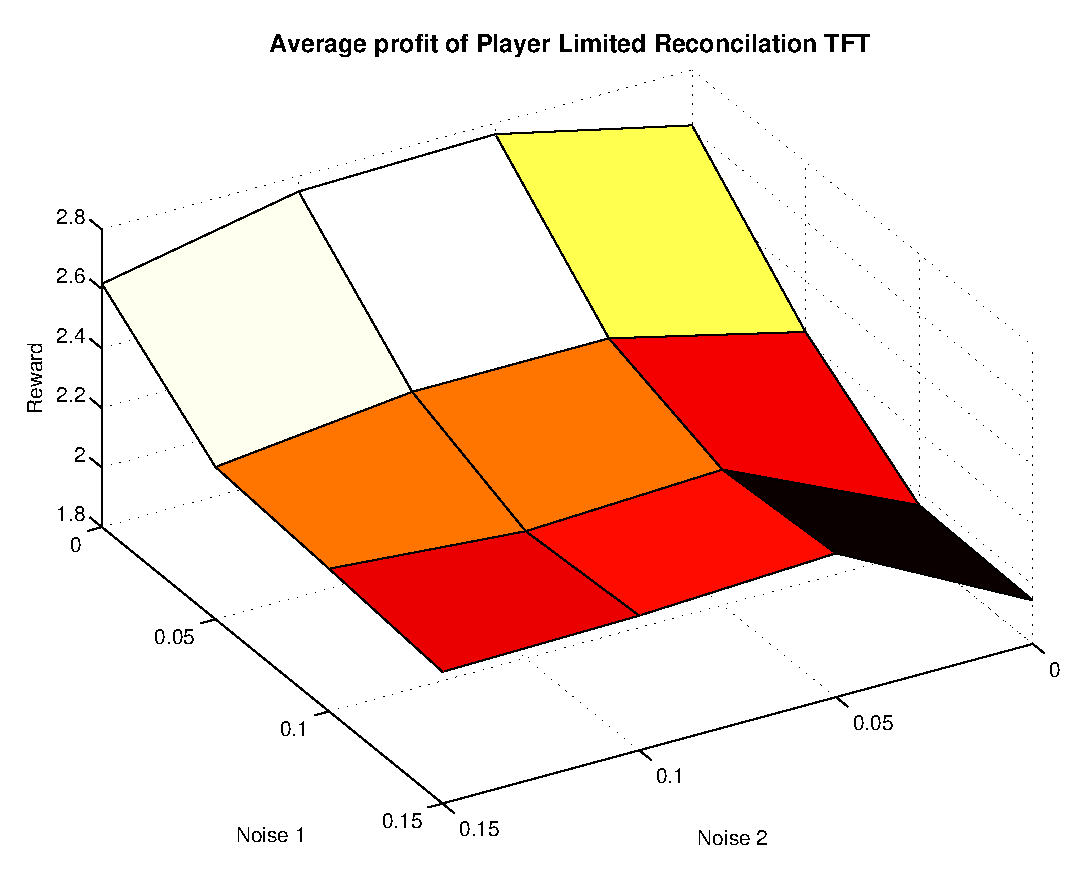
\includegraphics[width=\textwidth]{pics/simulation1/Reward_vs_Noise_of_Player_Limited_Reconcilation_TFT}
\end{minipage}
\hfill
\begin{minipage}[hbt]{0.3\textwidth}
	\centering
	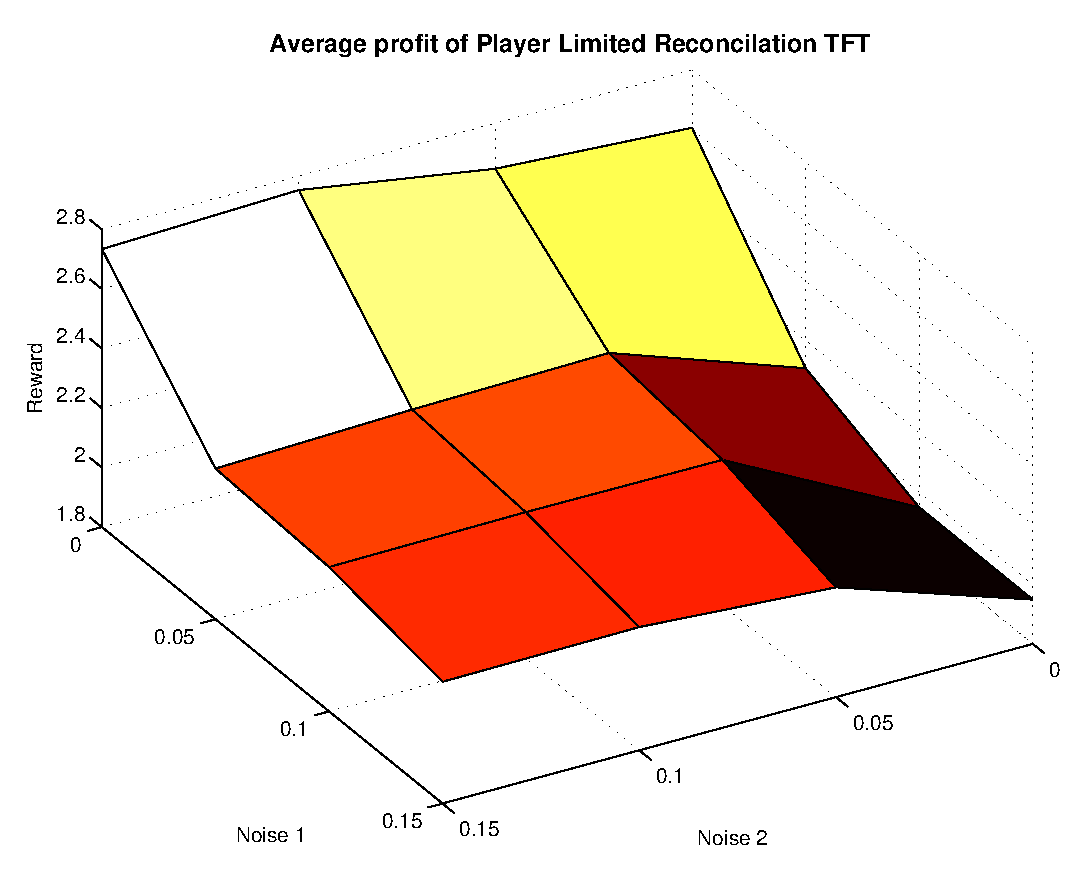
\includegraphics[width=\textwidth]{pics/simulation2/Reward_vs_Noise_of_Player_Limited_Reconcilation_TFT}
\end{minipage}	\caption{Reward versus Noise with the best players}
	\label{pic player best}
\end{figure}

At Noise1 equal zero the TFT mutants win, but for every noise1 larger than zero the strategy switcher wins, due to the small impact noise has on his performance.

In the following graphs the players performances are compared at zero noise, Noise1=0 and Noise2=0.15, Noise1=0.1 and Noise1=0 and both noises 0.1. The results are from the first simulation run.

Comparison of all players at zero noise:

\begin{figure}[h]

\begin{minipage}[hbt]{0.68\textwidth}
	\centering
	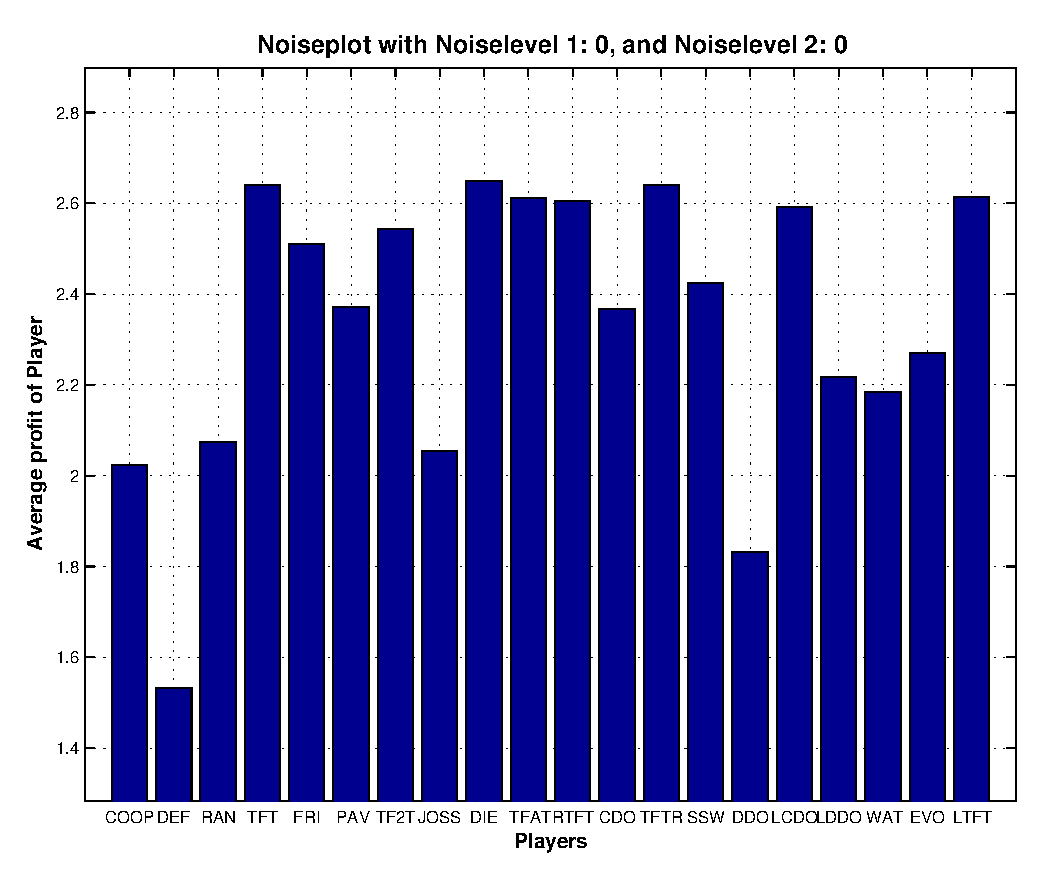
\includegraphics[width=\textwidth]{pics/simulation1/Reward_of__all_Players_at_given_Noiselevels_1}
\end{minipage}
\hfill
\begin{minipage}[hbt]{0.3\textwidth}
	\centering
	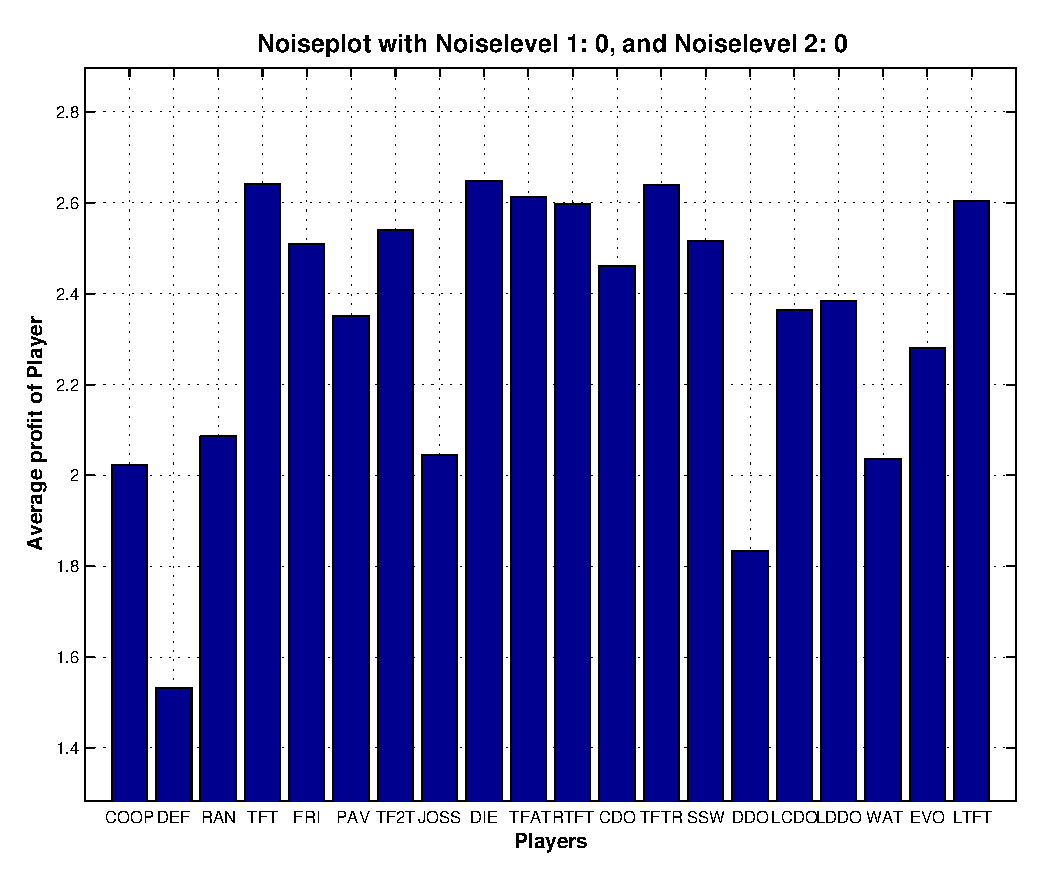
\includegraphics[width=\textwidth]{pics/simulation2/Reward_of_all_Players_at_given_Noiselevels_1}
\end{minipage}	\caption{Reward of players with both noises equals to zero}
	\label{pic player noise1}
\end{figure}

With no noise the best strategies are either TFT mutants, or variants of CDowning. Defective strategies perform poorly. This is in accordance to what Axelrod said: “Be nice”.

Noise1=0, Noise2=0.1

\begin{figure}[h]

\begin{minipage}[hbt]{0.68\textwidth}
	\centering
	\includegraphics[width=\textwidth]{pics/simulation1/Reward_of_all_Players_at_given_Noiselevels_2}
\end{minipage}
\hfill
\begin{minipage}[hbt]{0.3\textwidth}
	\centering
	\includegraphics[width=\textwidth]{pics/simulation2/Reward_of_all_Players_at_given_Noiselevels_2}
\end{minipage}	\caption{Reward of players with both noises equals to zero}
	\label{pic player noise1}
\end{figure}

The ranking of the different strategies does not change much. Generally everybody is profiting of the noise.
Noise1=0.1, Noise2=0

\begin{figure}[h]

\begin{minipage}[hbt]{0.68\textwidth}
	\centering
	\includegraphics[width=\textwidth]{pics/simulation1/Reward_of_all_Players_at_given_Noiselevels_3}
\end{minipage}
\hfill
\begin{minipage}[hbt]{0.3\textwidth}
	\centering
	\includegraphics[width=\textwidth]{pics/simulation2/Reward_of_all_Players_at_given_Noiselevels_3}
\end{minipage}	\caption{Reward of players with both noises equals to zero}
	\label{pic player noise1}
\end{figure}

The performance of the TFT mutants drastically decreases. Only Diekmann stays somewhat high. The strongest strategies are now the Lookback Downing and the strategy switcher. The strategy switcher before had the problem that the defections he tried out to exploit non-responding players cost him a lot. Now everybody sees defections due to the noise and it doesn’t matter that much anymore.

Noise1=0.1, Noise2=0.1

\begin{figure}[h]

\begin{minipage}[hbt]{0.68\textwidth}
	\centering
	\includegraphics[width=\textwidth]{pics/simulation1/Reward_of_all_Players_at_given_Noiselevels_4}
\end{minipage}
\hfill
\begin{minipage}[hbt]{0.3\textwidth}
	\centering
	\includegraphics[width=\textwidth]{pics/simulation2/Reward_of_all_Players_at_given_Noiselevels_4}
\end{minipage}	\caption{Reward of players with both noises equals to zero}
	\label{pic player noise1}
\end{figure}

The TFT mutants perform somewhat better than without Noise2, but the strategy switcher is still much stronger than the competition.






\clearpage

\section{Summary and Outlook}
The aim of this simulation was to investigate two things. The first was the impact of noise on the tournament. It turned out that Noise that lets Defections appear as cooperations is beneficial for most players. The opposite, when cooperative moves are perceived as defections, has a much larger impact. The performance of most friendly players drastically drops. It is especially harsh for players that relied on the effect of the first move being cooperative and have no mechanism to restore cooperation once it is lost.

The second investigated topic was how learning players would perform. Of the three learning mechanisms, copying others, Evolution and Strategy switching, Strategy switching performed the strongest. The strategy was also stronger than most not learning strategies. The other two approaches failed, because they were not responsive.

Outlook: The performance of the players was heavily impacted by the nature of the other players participating in the simulation. It would be interesting to run the simulation with more players. Another possible investigation could be to find out if the average performance increases with a noise that covers up defections forever, or if there is a turning point after which the performance decreases again.


\clearpage

\section{References}

\renewcommand{\refname}{}

\begin{thebibliography}{99}
	\bibitem{axelrod} 
		Axelrod, R., "Die Evolution der Kooperation". Munich: Oldenbourg Wissenschaftsverlag GmbH, German Edition (2000)

	\bibitem{github}
		\url{www.github.com}

	\bibitem{stanford}
		Kuhn, S., "Prisoner's Dilemma". URL: http://plato.stanford.edu/entries/prisoner-dilemma (accessed october 15, 2011)



	\bibitem{wu}
		Wu, J. et al, "How to Cope with Noise in the Iterated Prisoner's Dilemma". Journal of Conflict Resolution, Vol. 39, pages 183-189 (1995)

	\bibitem{donninger} 
		Donninger, C., "Is it always efficient to be nice?". Wien: Physica-Verlag Heidelverg (1986)
		%Internet: URL: www.socio.ethz.ch/vlib/pesb/pesb9.pdf

	\bibitem{joss}
		\url{www.socio.ethz.ch/vlib/pesb/pesb9.pdf}

	\bibitem{recon}
		\url{http://en.wikipedia.org/wiki/Evolution_of_cooperation#Axelrod.27s_Tournaments}




	\bibitem{nowak}
		Nowak, M., "Five Rules for the Evolution of Cooperation".  Science 314, page 1560 (2006)





	\bibitem{sandholm}
		Sandholm, T. et al, "Multiagent Reinforcement Learning in the Iterated Prisoner's Dilemma". Biosystems Vol 37, pages 147-166 (1995)

	\bibitem{quek}
		Queck, H. et al, "Adaptation of Iterated Prisoner's Dilemma Strategies by Evolution and Learning". Computational Intelligence and Games, pages: 40-47 (2007)





\end{thebibliography}

\clearpage

\appendix

\section{Submitted Researchplan}
\subsection{General Introduction}
Tournament like simulation of the prisoner's dilemma with repeated inter-
actions. Random errors are introduced in the information about the player's 
recent behavior. We want to observe the different outcome of the traditional
players if noise is introduced. Further we want to try to implement new 
players with learning strategies. \\
We believe that this makes the simulation more realistic.\\
Extension of Axelrod's Tournaments.

\subsection{Fundamental Questions}
Can a dispute based on miscommunication be overcome?\\
Can treason be hidden behind pretended miscommunication?\\
Does miscommunication discourage cooperation?\\
How much miscommunication can cooperation survive?\\
Do learning strategies have an advantage over the other ones?\\
How do the traditional players act and how does the final result change, 
if noise is introduced?\\
Independent variables: length of simulation, reliability of communication, rewards\\
Dependent variables: correlation between cooperation and success, frequency of cooperation, successful strategies

\subsection{Expected Results}
Miscommunication works against cooperating strategies.\\ 
Programs that reconcile are more successful.\\
The reward of the learning players is less influenced by the noise.

\subsection{References}

\begin{itemize}
\item On Evolving Robust Strategies for Iterated Prisoner's Dilemma, P. J. DARWEN and X. YAO, 16. November 1993\\
\item Multiagent Reinforcement Learning in the Iterated Prisoner's Dilemma, T. W. SANDHOLM and R. H. CRITES\\
\item Adaptation of Iterated Prisoner's Dilemma Strategies by Evolution and Learning, H. Y. QUEK and C. K. GOH, 2007\\
\item How to Cope with Noise in the Iterated Prisoner's Dilemma, J. WU and R. AXELROD, JOURNAL OF CONFLIC RTESOLUTION, Vol. 39 No. 1, March1995 183-189\\
\item Five Rules for the Evolution of Cooperation, M. A. NOWAK, Science 314, 1560 (2006)\\
\end{itemize}
\subsubsection{Research Methods}

Agent-Based Model

\subsection{Other}
The type(s) of the learning strategies we will decide later, after reading some of the literature.

\clearpage

\section{Matlabcode}

\subsection{Master.m}

\matlabscript{../matlab/Master}{Master.m}

\subsection{win.m}

\matlabscript{../matlab/win}{win.m}

\subsection{show\underline\ data.m}

\matlabscript{../matlab/show_data}{show\underline\ data.m}

\subsection{playerlist.m}

\matlabscript{../matlab/playerlist}{playerlist.m}

\subsection{player1.m}

\matlabscript{../matlab/player1}{player1.m}

\subsection{player2.m}

\matlabscript{../matlab/player2}{player2.m}

\subsection{player3.m}

\matlabscript{../matlab/player3}{player3.m}

\subsection{player4.m}

\matlabscript{../matlab/player4}{player4.m}

\subsection{player5.m}

\matlabscript{../matlab/player5}{player5.m}

\subsection{player6.m}

\matlabscript{../matlab/player6}{player6.m}

\subsection{player7.m}

\matlabscript{../matlab/player7}{player7.m}

\subsection{player8.m}

\matlabscript{../matlab/player8}{player8.m}

\subsection{player9.m}

\matlabscript{../matlab/player9}{player9.m}

\subsection{player10.m}

\matlabscript{../matlab/player10}{player10.m}

\subsection{player11.m}

\matlabscript{../matlab/player11}{player11.m}

\subsection{player12.m}

\matlabscript{../matlab/player12}{player12.m}

\subsection{player13.m}

\matlabscript{../matlab/player13}{player13.m}

\subsection{player14.m}

\matlabscript{../matlab/player14}{player14.m}

\subsection{player15.m}

\matlabscript{../matlab/player15}{player15.m}

\subsection{player16.m}

\matlabscript{../matlab/player16}{player16.m}

\subsection{player17.m}

\matlabscript{../matlab/player17}{player17.m}

\subsection{player18.m}

\matlabscript{../matlab/player18}{player18.m}

\subsection{player19.m}

\matlabscript{../matlab/player19}{player19.m}

\subsection{player20.m}

\matlabscript{../matlab/player20}{player20.m}






\end{document}  
git@github.com:Sandermatt/ETHAxelrodNoise.git